
\documentclass[
	12pt,				% tamanho da fonte
	openright,			% capítulos começam em pág ímpar (insere página vazia caso preciso)
	twoside,			% para impressão em recto e verso. Oposto a oneside
	a4paper,			% tamanho do papel. 
	% -- opções da classe abntex2 --
	chapter=TITLE,		% títulos de capítulos convertidos em letras maiúsculas
	%section=TITLE,		% títulos de seções convertidos em letras maiúsculas
	%subsection=TITLE,	% títulos de subseções convertidos em letras maiúsculas
	%subsubsection=TITLE,% títulos de subsubseções convertidos em letras maiúsculas
	% -- opções do pacote babel --
	english,			% idioma adicional para hifenização
	french,				% idioma adicional para hifenização
	spanish,			% idioma adicional para hifenização
	brazil,				% o último idioma é o principal do documento
	]{abntex2}


% ---
% PACOTES
% ---
\usepackage{fontawesome}
\usepackage{titlesec}
\usepackage{tikz}
\usepackage{xcolor}
\usepackage{colortbl}
\usepackage{pdflscape}
\usepackage{longtable, environ}
\usepackage{totcount}
\usepackage{caption}
\usepackage{pgf, calculator}
\usepackage{tikz}
\usepackage{ragged2e}

%saulo%



% ---
% Pacotes fundamentais 
% ---
%\usepackage{lmodern}			% Usa a fonte Latin Modern
\usepackage[T1]{fontenc}		% Selecao de codigos de fonte.
\usepackage[utf8]{inputenc}		% Codificacao do documento (conversão automática dos acentos)
\usepackage{indentfirst}		% Indenta o primeiro parágrafo de cada seção.
\usepackage{color}				% Controle das cores
\usepackage{graphicx}			% Inclusão de gráficos
\usepackage{microtype, breakurl} 			% para melhorias de justificação
% ---
\hyphenation{Téc-ni-co-ad-mi-nis-tra-ti-vo}
\PassOptionsToPackage{hyphens}{url}
\PassOptionsToPackage{hyphens}{url}
\usepackage{hyperref}
\usepackage{ifthen}


% ---
% Pacotes adicionais, usados no anexo do modelo de folha de identificação
% ---
\usepackage{multicol}
\usepackage{multirow}
\usepackage{hyperref}
% ---

\usepackage{array}

\newlength\Origarrayrulewidth

% horizontal rule equivalent to \cline but with 2pt width
\newcommand{\Cline}[1]{%
 \noalign{\global\setlength\Origarrayrulewidth{\arrayrulewidth}}%
 \noalign{\global\setlength\arrayrulewidth{2pt}}\cline{#1}%
 \noalign{\global\setlength\arrayrulewidth{\Origarrayrulewidth}}%
}

% draw a vertical rule of width 2pt on both sides of a cell
\newcommand\Thickvrule[1]{%
  \multicolumn{1}{!{\vrule width 2pt}c!{\vrule width 2pt}}{#1}%
}

% draw a vertical rule of width 2pt on the left side of a cell
\newcommand\Thickvrulel[1]{%
  \multicolumn{1}{!{\vrule width 2pt}c|}{#1}%
}

% draw a vertical rule of width 2pt on the right side of a cell
\newcommand\Thickvruler[1]{%
  \multicolumn{1}{|c!{\vrule width 2pt}}{#1}%
}

\setlength{\cftbeforesectionskip}{0em}
\setlength{\cftbeforechapterskip}{0.75em}




% ---
% Pacotes adicionais, usados apenas no âmbito do Modelo Canônico do abnteX2
% ---
\usepackage{lipsum}				% para geração de dummy text
% ---
\renewcommand{\sfdefault}{\rmdefault} % No serif fonts, use roman (times)
\renewcommand{\ABNTEXchapterfontsize}{\large}
\renewcommand{\ABNTEXsectionfontsize}{\normalsize}
\renewcommand{\ABNTEXsubsectionfontsize}{\normalsize}

\renewcommand{\ABNTEXchapterfont}{\bfseries}
\renewcommand{\ABNTEXsubsectionfont}{\bfseries\itshape}
\renewcommand{\ABNTEXsubsubsectionfont}{\itshape}
% ---
% Pacotes de citações
% ---
\usepackage[brazilian,hyperpageref]{backref}	 % Paginas com as citações na bibl
\usepackage[alf,  abnt-emphasize=bf]{abntex2cite}	% Citações padrão ABNT

% --- 
% CONFIGURAÇÕES DE PACOTES
% --- 

% ---
% Configurações do pacote backref
% Usado sem a opção hyperpageref de backref
\renewcommand{\backrefpagesname}{Citado na(s) página(s):~}
% Texto padrão antes do número das páginas
\renewcommand{\backref}{}
% Define os textos da citação
\renewcommand*{\backrefalt}[4]{
}%
%---


\newcommand{\quadroname}{Quadro}
\newcommand{\listofquadrosname}{Lista de quadros}

\newfloat[chapter]{quadro}{loq}{\quadroname}
\newlistof{listofquadros}{loq}{\listofquadrosname}
\newlistentry{quadro}{loq}{0}

% configurações para atender às regras da ABNT
\setfloatadjustment{quadro}{\centering}
\counterwithout{quadro}{chapter}
\renewcommand{\cftquadroname}{\quadroname\space} 
\renewcommand*{\cftquadroaftersnum}{\hfill--\hfill}

\setfloatlocations{quadro}{hbtp} % Ver https://github.com/abntex/abntex2/issues/176
% ---
\setlength{\cftbeforechapterskip}{0.6em}
\setlength{\cftbeforesubsectionskip}{0em}



% ---
% Informações de dados para CAPA e FOLHA DE ROSTO
% ---
\titulo{PROJETO PEDAGÓGICO DO CURSO TÉCNICO SUBSEQUENTE EM INFORMÁTICA  PARA INTERNET}
\autor{Equipe \abnTeX}
\local{}
\data{Tauá -- CE, 2024}
\instituicao{}
\tipotrabalho{}
% O preambulo deve conter o tipo do trabalho, o objetivo, 
% o nome da instituição e a área de concentração 
\preambulo{}
% ---
\def\UrlLeft{}
\def\UrlRight{}

\regtotcounter{section}
\newcommand{\nord}[1]{N$^\circ$ #1}

% ---
% Configurações de aparência do PDF final

% alterando o aspecto da cor azul
\definecolor{blue}{RGB}{41,5,195}

% informações do PDF
\makeatletter
\hypersetup{
     	%pagebackref=true,
		pdftitle={\@title}, 
		pdfauthor={\@author},
    	pdfsubject={\imprimirpreambulo},
	    pdfcreator={LaTeX with abnTeX2},
		pdfkeywords={abnt}{latex}{abntex}{abntex2}{relatório técnico}, 
		colorlinks=true,       		% false: boxed links; true: colored links
    	linkcolor=blue,          	% color of internal links
    	citecolor=blue,        		% color of links to bibliography
    	filecolor=magenta,      		% color of file links
		urlcolor=blue,
		bookmarksdepth=4
}
\makeatother
% --- 

% --- 
% Espaçamentos entre linhas e parágrafos 
% --- 

% O tamanho do parágrafo é dado por:
\setlength{\parindent}{1.3cm}

% Controle do espaçamento entre um parágrafo e outro:
\setlength{\parskip}{0.2cm}  % tente também \onelineskip

% ---
% compila o indice
% ---
\makeindex
% ---

% ----
% Início do documento
% ----


\renewcommand{\imprimircapa}{%
  \begin{center}
  
  
\includegraphics[width=.35\textwidth]{brasao_republica.jpg}
\par
MINISTÉRIO DA EDUCAÇÃO \par
SECRETARIA DE EDUCAÇÃO PROFISSIONAL E TECNOLÓGICA \par INSTITUTO FEDERAL DE EDUCAÇÃO, CIÊNCIA E TECNOLOGIA DO CEARÁ \par
{CAMPUS}  TAUÁ
    
    \vfill
    
  {\ABNTEXchapterfont\bfseries\Large
    PROJETO PEDAGÓGICO DO CURSO TÉCNICO \par 
    SUBSEQUENTE EM INFORMÁTICA \par 
    \vspace{0.3cm}
    PARA INTERNET
  }
  
  
  \vfill
  
   \thedate
  \end{center}
    \clearpage
}


\renewcommand{\imprimirfolhaderosto}{
  \begin{center}
  
\includegraphics[width=.25\textwidth]{logo-ifce-padrao.pdf}
\par
MINISTÉRIO DA EDUCAÇÃO \par
SECRETARIA DE EDUCAÇÃO PROFISSIONAL E TECNOLÓGICA \par INSTITUTO FEDERAL DE EDUCAÇÃO, CIÊNCIA E TECNOLOGIA DO CEARÁ \par
{CAMPUS} TAUÁ
    \vfill
    
    

    \begin{raggedright}
    
    \small
    {\bfseries REITOR} \\
    \MakeUppercase{José Wally Mendonça Menezes} \par

    {\bfseries PRÓ-REITORA DE ENSINO}\\
    \MakeUppercase{Cristiane Borges Braga} \par
    
    
    {\bfseries PRÓ-REITOR DE PESQUISA, PÓS-GRADUAÇÃO E INOVAÇÃO}\\
    \MakeUppercase{Joélia Marques de Carvalho} \par

    {\bfseries PRÓ-REITOR DE EXTENSÃO}\\
    \MakeUppercase{Ana Cláudia Uchôa} \par

    {\bfseries DIRETOR GERAL DO {CAMPUS} TAUÁ}\\
    JOSÉ ALVES DE OLIVEIRA NETO \par

    {\bfseries  CHEFE DE DEPARTAMENTO DE ENSINO DO {CAMPUS} TAUÁ}\\
    WEBERTE ALAN SOMBRA \par

    {\bfseries COORDENADOR DE PESQUISA   DO {CAMPUS} TAUÁ}\\
    TIAGO DE SOUSA LEITE \par
    
    {\bfseries COORDENADOR DE  EXTENSÃO DO {CAMPUS} TAUÁ}\\
    \MakeUppercase{Willame de Araújo Cavalcante} \par
    
    
     {\bfseries COORDENADOR DO CURSO TÉC. EM INFORMÁTICA PARA INTERNET}\\
    SAULO ANDERSON FREITAS DE OLIVEIRA \par
    
    
    \end{raggedright}
   \vfill
    
   
   
   \end{center}
   
    \cleardoublepage
    
    \begin{center}
  
\includegraphics[width=.25\textwidth]{logo-ifce-padrao.pdf}
\par
MINISTÉRIO DA EDUCAÇÃO \par
SECRETARIA DE EDUCAÇÃO PROFISSIONAL E TECNOLÓGICA \par INSTITUTO FEDERAL DE EDUCAÇÃO, CIÊNCIA E TECNOLOGIA DO CEARÁ \par
{CAMPUS} TAUÁ
    \vfill
    
    \begin{raggedright}

    \small
    {\centering
    {\bfseries COMISSÃO DE ELABORA\c{C}\~AO DO PROJETO PEDAG\'OGICO DO CURSO  } \\
    PORTARIA N\textordmasculine\ 163/GAB-TAU/DG-TAU/TAUA, DE 11 DE DEZEMBRO DE 2019 \par
    }
    

\vfill

    
     {\bfseries REPRESENTANTE PELO ENSINO DO {CAMPUS}}\\
    WEBERTE ALAN SOMBRA \par
    
     {\bfseries COORDENADOR DO CURSO}\\
    SAULO ANDERSON FREITAS DE OLIVEIRA \par
    
    {\bfseries PEDAGOGA}\\
    PRUCINA DE CARVALHO BEZERRA \par
    
    
    {\bfseries BIBLIOTECÁRIA}\\
    ANALICE FRAGA DE OLIVEIRA  \par
    
    {\bfseries PROFESSOR DA ÁREA DIVERSIFICADA}\\
    ANELISE DANIELA SCHINAIDER \par
    
    
    {\bfseries PROFESSOR DA ÁREA TÉCNICA}\\
    LUCAS FERREIRA MENDES \par
    
    
    {\bfseries PROFESSOR DA ÁREA TÉCNICA}\\
    ANT\^ONIO S\'AVIO SILVA OLIVEIRA \par
    
    {\bfseries PROFESSOR DA ÁREA TÉCNICA}\\
    J\'ULIO SERAFIM MARTINS \par
    
    {\bfseries COORDENADORA NEABI}\\
    MARGARIDA MARIA XAVIER DA SILVA \par
    
    {\bfseries COORDENADORA NAPNE}\\
    SHARLENE PAREIRA ALVES \par
    
    {\bfseries COORDENADORA NUGEDS}\\
    CARLOS GET\'ULIO DE FREITAS MAIA\par
    
    
    % Saulo Anderson Freitas De Oliveira -- {\bfseries Coordenador do Curso} \par
    
    % Prucina de Carvalho Bezerra -- {\bfseries Pedagoga} \par
    
    % Analice Fraga de Oliveira -- {\bfseries Bibliotecária} \par

    % Jefferson Calixto Figueiredo -- {\bfseries Professor da área técnica} \par
    
    
    % Lucas Ferreira Mendes -- {\bfseries Professor da área técnica}


   
   \end{raggedright}
   \vfill
    
   
   \end{center}
   
    \cleardoublepage

}


%%%% DOCENTES & TeC



\newcommand{\docente}[5]{

    \multicolumn{3}{l}{\cellcolor{gray!15}\bfseries \uppercase{#1}} \\
    
    \multicolumn{3}{l}{#2} \\
    
    \multicolumn{1}{l}{ \cellcolor{gray!05}\bfseries  REGIME DE TRABALHO} & \multicolumn{1}{l}{ \cellcolor{gray!05}\bfseries  VÍNCULO} & \multicolumn{1}{l}{ \cellcolor{gray!05}\bfseries  PERFIL DOCENTE} \\

    
    \multicolumn{1}{l}{Dedicação Exclusiva} & \multicolumn{1}{l}{Efetivo} & \multicolumn{1}{l}{#4}\\
    
    \multicolumn{3}{l}{\cellcolor{gray!05}\bfseries  FORMAÇÃO ACADÊMICA} \\
    
    \multicolumn{3}{l}{#3} \\\\

}



\newcommand{\docentex}[5]{

    \multicolumn{3}{l}{\cellcolor{gray!15}\bfseries \uppercase{#1}} \\
    
    \multicolumn{3}{l}{#2} \\
    
    \multicolumn{1}{l}{ \cellcolor{gray!05}\bfseries  REGIME DE TRABALHO} & \multicolumn{1}{l}{ \cellcolor{gray!05}\bfseries  VÍNCULO} & \multicolumn{1}{l}{ \cellcolor{gray!05}\bfseries  PERFIL DOCENTE} \\
   

    
    \multirow{1}{*}{Dedicação Exclusiva} & \multirow{1}{*}{Efetivo} & \multirow{1}{*}{#4}\\
    & & #5 \\
    
    
    \multicolumn{3}{l}{\cellcolor{gray!05}\bfseries  FORMAÇÃO ACADÊMICA} \\
    
    \multicolumn{3}{l}{#3} \\\\

}
%
%
%\newcommand{\docentev}[5]{
%
%    \multicolumn{3}{l}{\cellcolor{gray!15}\bfseries \uppercase{#1}} \\
%    
%    \multicolumn{3}{l}{#2} \\
%    
%    \multicolumn{1}{l}{ \cellcolor{gray!05}\bfseries  REGIME DE TRABALHO} & \multicolumn{1}{l}{ \cellcolor{gray!05}\bfseries  VÍNCULO} & \multicolumn{1}{l}{ \cellcolor{gray!05}\bfseries  PERFIL DOCENTE} \\
%   
%
%    
%    \multirow{1}{*}{20 Horas} & \multirow{1}{*}{Efetivo} & \multirow{1}{*}{#4}\\
%    
%    
%    \multicolumn{3}{l}{\cellcolor{gray!05}\bfseries  FORMAÇÃO ACADÊMICA} \\
%    
%    \multicolumn{3}{l}{#3} \\\\
%
%}

\newcommand{\doc}[5]{

    \multicolumn{3}{ p{\textwidth-2\tabcolsep} }{\cellcolor{gray!15}\bfseries \uppercase{#1}} \\
    
    \multicolumn{3}{ p{\textwidth-2\tabcolsep} }{#2} \\
    
    \multicolumn{1}{ p{.378\textwidth-2\tabcolsep} }{ \cellcolor{gray!05}\bfseries  REGIME DE TRABALHO} &
    \multicolumn{1}{ p{.16\textwidth-2\tabcolsep} }{ \cellcolor{gray!05}\bfseries  VÍNCULO} &
    \multicolumn{1}{ p{.46\textwidth-2\tabcolsep} }{ \cellcolor{gray!05}\bfseries  PERFIL DOCENTE} \\

    
    \multicolumn{1}{ p{.378\textwidth-2\tabcolsep} }{Dedicação Exclusiva} & 
    \multicolumn{1}{ p{.16\textwidth-2\tabcolsep} }{Efetivo} & 
    \multicolumn{1}{ p{.46\textwidth-2\tabcolsep} }{#4}\\
    
    \multicolumn{3}{ p{\textwidth-2\tabcolsep} }{\cellcolor{gray!05}\bfseries  FORMAÇÃO ACADÊMICA} \\
    
    \multicolumn{3}{ p{\textwidth-2\tabcolsep} }{#3} \\[1em]

}

\newcommand{\docv}[5]{

    \multicolumn{3}{ p{\textwidth-2\tabcolsep} }{\cellcolor{gray!15}\bfseries \uppercase{#1}} \\
    
    \multicolumn{3}{ p{\textwidth-2\tabcolsep} }{#2} \\
    
    \multicolumn{1}{ p{.378\textwidth-2\tabcolsep} }{ \cellcolor{gray!05}\bfseries  REGIME DE TRABALHO} &
    \multicolumn{1}{ p{.16\textwidth-2\tabcolsep} }{ \cellcolor{gray!05}\bfseries  VÍNCULO} &
    \multicolumn{1}{ p{.46\textwidth-2\tabcolsep} }{ \cellcolor{gray!05}\bfseries  PERFIL DOCENTE} \\

    
    \multicolumn{1}{ p{.378\textwidth-2\tabcolsep} }{20 Horas} & 
    \multicolumn{1}{ p{.16\textwidth-2\tabcolsep} }{Efetivo} & 
    \multicolumn{1}{ p{.46\textwidth-2\tabcolsep} }{#4}\\
    
    \multicolumn{3}{ p{\textwidth-2\tabcolsep} }{\cellcolor{gray!05}\bfseries  FORMAÇÃO ACADÊMICA} \\
    
    \multicolumn{3}{ p{\textwidth-2\tabcolsep} }{#3} \\[1em]

}




\newcommand{\tecn}[4]{

	
    \multicolumn{2}{ p{\textwidth-2\tabcolsep} }{\cellcolor{gray!15}\bfseries \uppercase{#1}} \\
    
    \multicolumn{2}{ p{\textwidth-2\tabcolsep} }{#2} \\
    
    \multicolumn{1}{ p{.5\textwidth-2\tabcolsep} }{ \cellcolor{gray!05}\bfseries TITULAÇÃO MÁXIMA} &
    \multicolumn{1}{ p{.5\textwidth-2\tabcolsep} }{ \cellcolor{gray!05}\bfseries  ATIVIDADE DESENVOLVIDA}  \\

    
    \multicolumn{1}{ p{.5\textwidth-2\tabcolsep} }{#3} &
    \multicolumn{1}{ p{.5\textwidth-2\tabcolsep} }{#4} \\[0.5em]



}

\newcommand{\altera}[1]{
	{\color{red}{#1}}
}

\newcommand{\tecnico}[4]{

    \multicolumn{2}{l}{\cellcolor{gray!15}\bfseries \uppercase{#1}} \\
    
    \multicolumn{2}{l}{#2} \\
    
    \multicolumn{1}{l}{ \cellcolor{gray!05}\bfseries TITULAÇÃO MÁXIMA} & \multicolumn{1}{l}{ \cellcolor{gray!05}\bfseries  ATIVIDADE DESENVOLVIDA}  \\

    
    \multicolumn{1}{l}{#3} & \multicolumn{1}{l}{#4} \\\\

}

\newenvironment{listadocente}
    {\noindent
\begin{tabular}{l p{.2\linewidth}  p{.3\linewidth} }
    }
    { 
    \\
    \end{tabular}
    }
%--------------------------------------------------


\newenvironment{listadtecnicos}
    {\noindent
\begin{tabular}{p{.44\linewidth} p{.44\linewidth} }
    }
    { 
    \\
    \end{tabular}
    }
%--------------------------------------------------





\begin{document}


% Seleciona o idioma do documento (conforme pacotes do babel)
%\selectlanguage{english}
\selectlanguage{brazil}

% Retira espaço extra obsoleto entre as frases.
\frenchspacing 

% ----------------------------------------------------------
% ELEMENTOS PRÉ-TEXTUAIS
% ----------------------------------------------------------
% \pretextual

% ---
% Capa
% ---
\imprimircapa
\cleardoublepage
% ---

% ---
% Folha de rosto
% (o * indica que haverá a ficha bibliográfica)
% ---
\imprimirfolhaderosto

% ---

% ---
% Anverso da folha de rosto:
% ---


% ---
% inserir o sumario
% ---
\pdfbookmark[0]{\contentsname}{toc}
\setlength{\beforechapskip}{0pt}
\tableofcontents*
\cleardoublepage
% ---


\thispagestyle{empty}

\pretextual
\begin{center}
	\ABNTEXchapterfont\large\textbf{DADOS DO CURSO}
\end{center}

%\section*{Identificação da Instituição de Ensino}
\small
\noindent
\begin{tabularx}{\linewidth}{X X X X }
    
    \multicolumn{4}{c}{\textbf{IDENTIFICAÇÃO DA INSTITUIÇÃO DE ENSINO}} \\
    \toprule
    \multicolumn{4}{l}{\cellcolor{gray!20}\textbf{Nome:}} \\
    \multicolumn{4}{l}{Instituto Federal de Educação, Ciência e Tecnologia do Ceará -- \textit{campus} Tauá} \\
    
    \multicolumn{4}{l}{\cellcolor{gray!20}\textbf{CNPJ:}} \\
    \multicolumn{4}{l}{10.744.098/0015-40} \\
    
    \multicolumn{4}{l}{\cellcolor{gray!20}\textbf{Endere\c{c}o:}} \\
    \multicolumn{4}{l}{Rua Antônio Teixeira Benevides, 01, Bairro Colibris -- CEP: 63660-000} \\
    
    
     
    \multicolumn{2}{l}{\cellcolor{gray!20}\textbf{CIDADE}} & \cellcolor{gray!20} \textbf{UF} & \cellcolor{gray!20} \textbf{TELEFONE} \\
     
    \multicolumn{2}{l}{Tauá} & Ceará & (88) 3437-4249\\

     \multicolumn{2}{l}{\cellcolor{gray!20}\textbf{PÁGINA INSTITUCIONAL}} &
     \multicolumn{2}{l}{\cellcolor{gray!20}\textbf{E-MAILS}} \\
     
     \multicolumn{2}{l}{\href{http://ifce.edu.br/taua}{ifce.edu.br/taua}} &
     \multicolumn{2}{l}{\href{mailto:cinformaticainternet@taua.ifce.edu.br}{cinformaticainternet@taua.ifce.edu.br}} \\
     
     \bottomrule
     
\end{tabularx}
\vspace{2em}
\noindent

\begin{tabularx}{\linewidth}{X X}
	\multicolumn{2}{c}{\cellcolor{gray!10}\textbf{Informações sobre carga horária do curso}} \\
	
	\cellcolor{gray!10}\textbf{Carga horária total para integralização} &
	\cellcolor{gray!10}\textbf{Carga horária dos componentes curriculares (disciplinas)} \\
	
	1000h & 1000h\\
	
	\cellcolor{gray!10}\textbf{Carga horária dos componentes curriculares optativos} &
	\cellcolor{gray!10}\textbf{Carga horária total da Prática Profissional Supervisionada no curso} \\
	
	120h & 40h\\
	
	 
\end{tabularx}

% 
% \begin{tabularx}{\linewidth}{X X X X X X}
%     
%     
%         \multicolumn{6}{c}{\textbf{INFORMAÇÕES GERAIS DO CURSO}} \\
% \toprule
%     \multicolumn{6}{l}{\cellcolor{gray!20}\textbf{DENOMINAÇÃO DO CURSO}} \\
%     
%     \multicolumn{6}{l}{Curso Técnico Subsequente em Informática para Internet} \\
%     
%         
%     \multicolumn{6}{l}{\cellcolor{gray!20}\textbf{TITULAÇÃO CONFERIDA}} \\
%     
%     \multicolumn{6}{l}{Técnico em Informática para Internet} \\
%     
%     %%%%%
%     \multicolumn{1}{l}{\cellcolor{gray!20}\textbf{NÍVEL}} & \multicolumn{5}{l}{\cellcolor{gray!20}\textbf{\qquad~FORMA DE ARTICULAÇÃO COM O ENSINO MÉDIO}} \\
%     
%     \multicolumn{1}{l}{Médio} & \multicolumn{5}{l}{\qquad~~Subsequente} \\
%     
%     %%%%%
%     \multicolumn{3}{ p{.5\linewidth-2\tabcolsep }  }{\cellcolor{gray!20}\textbf{MODALIDADE DE ENSINO}} & \multicolumn{3}{ p{.5\linewidth-2\tabcolsep } }{\cellcolor{gray!20}\textbf{DURAÇÃO DO CURSO}} \\
%     
%     \multicolumn{3}{l}{Presencial} & \multicolumn{3}{l}{Entre 3 e 6 semestres -- 1,5 anos} \\
%     %%%%
%     \multicolumn{3}{l}{\cellcolor{gray!20}\textbf{PERIODICIDADE}} & \multicolumn{3}{l}{\cellcolor{gray!20}\textbf{FORMA DE INGRESSO}} \\ 
%     
%     \multicolumn{3}{l}{Semestral} & \multicolumn{3}{l}{Processo Seletivo Regular, Diplomados,} \\
% 
%    \multicolumn{3}{l}{} & \multicolumn{3}{l}{Transferência e Matrícula Especial.} \\
%      
%      
%       %%%%
%     \multicolumn{3}{l}{\cellcolor{gray!20}\textbf{NÚMERO DE VAGAS ANUAIS}} & \multicolumn{3}{l}{\cellcolor{gray!20}\textbf{TURNO DE FUNCIONAMENTO}} \\ 
%     
%     \multicolumn{3}{l}{60} & \multicolumn{3}{l}{Noturno} \\
%     
%     
%     \multicolumn{6}{l}{\cellcolor{gray!20}\textbf{ANO E SEMESTRE DO INÍCIO DO FUNCIONAMENTO}} \\
%     
%     \multicolumn{6}{l}{2022.1} \\
%     
%     
%     
%     \multicolumn{2}{l}{\cellcolor{gray!20}\textbf{CARGA HORÁRIA TOTAL}} &
%     \multicolumn{4}{l}{\cellcolor{gray!20}\textbf{CARGA HORÁRIA DOS COMPONENTES CURRICULARES}} \\
%     
%     \multicolumn{2}{l}{1200 horas-aula (1000 horas)} &
%     \multicolumn{4}{l}{1200 horas-aula (1000 horas)} 
%      \\
% 
%     
%     
%     %%%%%
%     
%     
%     
%      
%     \multicolumn{6}{l}{\cellcolor{gray!20}\textbf{CARGA HORÁRIA TOTAL DA PRÁTICA PROFISSIONAL}} \\
%     
%     \multicolumn{6}{l}{~160 horas-aula (133 horas e 20 minutos)} \\
%     
%     
%       %%%%
%     \multicolumn{3}{l}{\cellcolor{gray!20}\textbf{SISTEMA DE CARGA HORÁRIA}} & \multicolumn{3}{l}{\cellcolor{gray!20}\textbf{DURAÇÃO DA HORA-AULA}} \\ 
%     
%     \multicolumn{3}{l}{1 crédito = 20 horas-aula} & \multicolumn{3}{l}{50 minutos} \\
%     
%     
%     \bottomrule
%     
%     % \textbf{Denominação} & Curso Técnico Subsequente em Informática para Internet \\ \hline
%     
%     % \textbf{Titulação conferida} &  Técnico  em Informática para \newline Internet \\ \hline
%     
%     % \textbf{Nível} &  M\'edio \\ \hline
%     
%     % % \textbf{Forma de articulação com o Ensino Médio} &  Subsequente \\ \hline
%     
%     % \textbf{Modalidade de oferta} & Presencial \\ \hline
%     
%     % \textbf{Duração} &  1 ano e meio (18 meses) \\ \hline
%     
%     % \textbf{Periodicidade} &  Semestral \\ \hline
%     
%     % \textbf{Forma de ingresso} &  Processo seletivo \\ \hline
%     
%     % \textbf{Número de vagas anuais} &  50 \\ \hline
%     
%     % \textbf{Turno de funcionamento} &  Integral \\ \hline
%     
%     % \textbf{Ano e semestre do início do funcionamento} &  2021.1 \\ \hline
%     
%     % \textbf{Carga horária dos componentes curriculares (disciplinas)} &  Integral \\ \hline
%     
%     % \textbf{Carga horária da prática profissional} &  100 horas \\ \hline
%     
%     %  \textbf{Carga horária total} &  100 horas \\ \hline
%     
%     
%     %  \textbf{Sistema de carga horária} &  1 crédito = 20 horas \\ \hline
%     
%     %     \textbf{Duração da hora-aula} & 50 minutos \\ \hline
% 
% \end{tabularx}
% 
% 


% ----------------------------------------------------------
% ELEMENTOS TEXTUAIS
% ----------------------------------------------------------

% ----------------------------------------------------------
% Introdução (exemplo de capítulo sem numeração, mas presente no Sumário)
% ----------------------------------------------------------
\makeheadrule{abntheadings}{0\textwidth}{\normalrulethickness}
\makeevenhead{abntheadings}{\ABNTEXfontereduzida\thepage}{}{}
\makeoddhead{abntheadings}{}{}{\ABNTEXfontereduzida\thepage}

\pagestyle{abntheadings}


\textual


\normalsize


	% CAPS 
	% 1 APRESENTAÇÃO
	% 2 CONTEXTUALIZAÇÃO DA INSTITUIÇÃO
	% 3 JUSTIFICATIVA PARA A CRIAÇÃO DO CURSO 
	
\chapter{Apresentação}


%  
 
 O Projeto Pedagógico de um curso é o documento que expressa a sua identidade.
 Tem como finalidade precípua apresentar à comunidade acadêmica como o curso
 caracteriza-se e organiza-se, em função de suas escolhas e percursos, para
 contribuir na formação profissional que se propõe a oferecer aos discentes.
 
 Nesse sentido, o presente documento versa sobre o projeto pedagógico do Curso
 Técnico Subsequente em Informática para Internet do Instituto Federal de
 Educação, Ciência e Tecnologia do Ceará, \textit{campus} Tauá, e está
 fundamentado nas bases legais e nos princípios norteadores que regulamentam a
 educação profissional de nível médio.
 
 
 A idealização deste curso foi feita por meio do projeto de expansão do
 \textit{campus} Tauá, pensando em atender e melhorar seu atendimento ao município
 de Tauá e municípios vizinhos. 
 Foi observado que há na região demanda reprimida de alunos que
 não possuíam dimensões profissionalizantes. Assim, movido pelo seu Plano de Desenvolvimento da Instituição, que tem por
 objetivo expandir as possibilidades de oferta de cursos na comunidade visando
 um melhor desenvolvimento tecnológico e interdisciplinar, o \textit{campus} Tauá, que já tinha o parecer favorável à implantação 
 do Curso Técnico em Informática para Internet, na modalidade subsequente, deu início às tratativas da criação do referido curso.
 
 
 Para o processo de alteração do PPC, foi instituída uma comissão, mediante
 Portaria \nord{2275}/GAB-TAU/DG-TAU/TAUA, DE 05 DE ABRIL DE 2024, composta pelos professores
 Anelise Daniela Schinaider, Antônio Sávio Silva Oliveira, Júlio Serafim Margins, Lucas Ferreira Mendes e Saulo Anderson Freitas de
 Oliveira, a pedagoga Prucina de Carvalho Bezerra,  a  bibliotecária-documentalista 
Analice Fraga de Oliveira, a coordenadora do NEABI Margarida Maria Xavier da Silva, a coordenadora do NAPNE Sharlene Pereira Alves e o coordenador do NUGED Carlos Getúlio de Freitas Maia. Os membros atuaram  em diversas reuniões, observando a legislação vigente, construíram o
 presente documento. Foi dada atenção especial aos Programas de Unidades Didáticas
 e as cargas horárias das disciplinas para gerar compatibilidade com o curso Superior de Tecnologia em Análise e Desenvolvimento de Sistemas, de maneira a melhor distribuir as trilhas de conhecimento junto à complexidade delas pelo curso e à verticalização do Ensino para os concludentes.
 
 

 


 
 % A elaboração deste projeto pedagógico teve como primeiro procedimento
 % metodológico a pesquisa documental nas leis, decretos e resoluções acerca da
 % criação e oferta de cursos subsequentes pelas Instituições Federais. Com
 % isso, delimitou-se a base pedagógica e normativa para o curso subsequente a
 % ser ofertado no Campus Tauá.
 Além disso, contou-se com as orientações pertinentes nas normativas
 institucionais no âmbito dos cursos técnicos, tais como, o Regulamento da
 Organização Didática do IFCE (ROD) e  o Plano de Desenvolvimento Institucional
 do IFCE (PDI) e o Projeto Político-Pedagógico Institucional (PPI).
% \begin{itemize} \setlength\itemsep{0em} \item Regulamento da Organização
% Didática no IFCE -- ROD; \item Plano de Desenvolvimento Institucional do IFCE
% -- PDI; \item Projeto Pedagógico Institucional -- PPI.
% \end{itemize}
 

O documento está organizado em dez (10) seções, a saber: Apresentação, Contextualização da Instituição, Justificativa para a Criação do Curso, Fundamentação Legal, Objetivos do Curso, Organização do Curso, Avaliação do Projeto do Curso, Políticas Institucionais Constantes no PDI, Apoio ao Docente, e, por fim, Infraestrutura.


Inicialmente, nas seções Contextualização da Instituição e Justificativa para a Criação do Curso são descritos um breve histórico da Instituição e do \textit{campus} Tauá, a justificativa para criação do curso e os princípios norteadores regionais que guiam a proposta de implantação deste curso. Em seguida, apresenta-se a fundamentação legal, os objetivos e os itens que compõem a organização do curso, tais como: as formas de ingresso, as áreas de atuação e o perfil esperado do futuro profissional. Logo após, é apresentada a  matriz curricular e seu fluxograma, os aspectos referentes à avaliação da aprendizagem, à prática profissional, ao aproveitamento de conhecimentos, à emissão de diploma, ao perfil docente e ao rodízio nas unidades curriculares. Aborda-se ainda, sobre projetos integradores, atividades complementares, metodologias empregadas no ensino e sua integração \`a pesquisa e extensão.

Logo depois, são abordados aspectos  da avaliação do projeto do curso e as metas que serão oportunizadas dentro do Plano de Desenvolvimento Institucional do \textit{campus} Tauá. Continuando, são elencadas ações estratégicas de apoio ao discente através dos setores existentes, apresentando o corpo docente necessário para a execução do curso. Na sequência, a seção Infraestrutura descreve as instalações e espaços disponibilizados pelo \textit{campus} para as diversas atividades inerentes ao dia-a-dia do curso. Por fim, os anexos detalham os Programas de Unidade Didática (PUDs) das disciplinas que formam a matriz curricular do curso e demais anexos referentes à organização da Instituição e do curso.


\chapter{Contextualização da instituição}

\section{Finalidades do Instituto Federal de Educação, Ciência e Tecnologia do Ceará}


O Instituto Federal de Educação, Ciência e Tecnologia do Ceará (IFCE) é uma Instituição Tecnológica que tem como marco referencial de sua história a evolução contínua com crescentes indicadores de qualidade. A sua trajetória corresponde ao processo histórico de desenvolvimento industrial e tecnológico da Região Nordeste e do Brasil.

A história institucional inicia-se no século XX, quando o então Presidente Nilo Peçanha cria, mediante o Decreto n$^\circ$  7.566, de 23 de setembro de 1909, as Escolas de Aprendizes Artífices, com a inspiração orientada pelas escolas vocacionais francesas, destinadas a atender à formação profissional aos pobres e desvalidos da sorte. O incipiente processo de industrialização passa a ganhar maior impulso durante os anos 40, em decorrência do ambiente gerado pela II Guerra Mundial, levando à transformação da Escola de Aprendizes Artífices em Liceu Industrial de Fortaleza, no ano de 1941 e, no ano seguinte, passa a ser chamado de Escola Industrial de Fortaleza, passando a ofertar formação profissional diferenciada das artes e ofícios, mas orientada para atender às profissões básicas do ambiente industrial e ao processo de modernização do País.

O crescente processo de industrialização, mantido por meio da importação de tecnologias orientadas para a substituição de produtos importados, gerou a necessidade de formar mão de obra técnica para operar esses novos sistemas industriais e para atender às necessidades governamentais de investimento em infraestrutura. No ambiente desenvolvimentista da década de 50, a Escola Industrial de Fortaleza, mediante a Lei Federal n$^\circ$ 3.552, de 16 de fevereiro de 1959, ganhou a personalidade jurídica de Autarquia Federal, passando a gozar de autonomia administrativa, patrimonial, financeira, didática e disciplinar, incorporando a missão de formar profissionais técnicos de nível médio.

Em 1965, passa a se chamar Escola Industrial Federal do Ceará e em 1968, recebe então a denominação de Escola Técnica Federal do Ceará, demarcando o início de uma trajetória de consolidação de sua imagem como instituição de educação profissional, com elevada qualidade, passando a ofertar cursos técnicos de nível médio nas áreas de Edificações, Estradas, Eletrotécnica, Mecânica, Química Industrial, Telecomunicações e Turismo.


O contínuo avanço do processo de industrialização, com crescente complexidade tecnológica, orientada para a exportação, originou a demanda de evolução da Rede de Escolas Técnicas Federais, já no final dos anos 70, para a criação de um novo modelo institucional, surgindo então os Centros Federais de Educação Tecnológica – CEFET's.


A partir da Lei 11.892, de 29 de dezembro de 2008, sancionada pelo então
presidente Luiz Inácio Lula da Silva, passou \`a denominação de Instituto
Federal de Educação, Ciência e Tecnologia do Ceará, mediante integração do
Centro Federal de Educação Tecnológica do Ceará e das Escolas Agrotécnicas
Federais de Crato e de Iguatu, tendo hoje 35 unidades (34 \textit{campi} e Reitoria), distribuídas em todas as
regiões do Estado.
Ao longo da história, os Institutos Federais tornaram-se instituições de
educação superior, básica e profissional, pluricurriculares e multicampi,
especializados na oferta de educação profissional e tecnológica nas diferentes
modalidades de ensino, com base na conjugação de conhecimentos técnicos e
tecnológicos com práticas pedagógicas.

% O campus de Tauá, do Instituto Federal de Educação, Ciência e Tecnologia do Ceará (IFCE), foi inaugurado em 20 de novembro de 2009, como um campus avançado do IFCE de Crateús. Situado em Tauá, município polo da região do sertão dos Inhamuns, distante 334 km de Fortaleza, abrange os municípios de Quiterianópolis, Parambu, Arneiroz e Aiuaba, recebendo também alunos de várias outras regiões, por meio do Sistema de Seleção Unificada (SISU) do Ministério da Educação (MEC), e outros processos seletivos que se fizerem necessários conforme a demanda.


\section{Histórico e Estrutura do IFCE \textit{campus} Tauá}

O \textit{campus} Tauá do IFCE foi inaugurado em 20 de novembro de 2009 como um \textit{campus} avançado do IFCE de Crateús. Situado na cidade de Tauá, município-polo da região Sertão dos Inhamuns, distante 334 $\mathrm{km}$ de Fortaleza, abrange os municípios de Arneiroz, Aiuaba, Parambu e Quiterianópolis \cite{ipece17}, e recebe alunos de várias outras regiões, por meio do Sistema de Seleção Unificada (SISU) do Ministério da Educação (MEC), e outros processos seletivos.

Mesmo antes da inauguração, começaram as tratativas para a definição dos primeiros cursos e serviços a serem ofertados pelo \textit{campus} Tauá. Após uma ampla discussão com a sociedade, ficou definido que, inicialmente, haveria a oferta de dois cursos, um de nível técnico em Agronegócio e outro de nível superior em Tecnologia em Telemática (criado pela Resolução 23/2010 do CONSUP/IFCE, em 31 de maio de 2010).

Procedeu-se à organização de um vestibular e um exame de seleção que, após divulgação e realização, possibilitou o ingresso dos primeiros alunos, ocorrendo inicialmente a oferta de 70 vagas, 35 para cada curso. As primeiras turmas iniciaram as atividades em setembro de 2010 e, semestralmente, novos ingressos foram promovidos, sendo que, para o curso de Telemática, o acesso passou a ser realizado através do SISU/MEC.

Com a adesão ao Programa Nacional de Acesso ao Ensino Técnico e Emprego (PRONATEC), em 2012, o \textit{campus} Tauá passou a ofertar, de forma concomitante, aos alunos do ensino médio da região, um Curso Técnico de Informática, curso este que teve uma oferta única com 40 vagas. Ainda em 2012, o \textit{campus} começou a promover eventos de extensão voltados à divulgação da instituição e fortalecimento das atividades acadêmicas, com destaque para o I Encontro de Tecnologia em Telemática (TECTEL), que passa a ser realizado anualmente pelo curso de Telemática, e a I Semana do Agronegócio, o que inclusive possibilitou o aumento de parcerias com organizações públicas e privadas.

Em 2013, o \textit{campus} Tauá deixou de ser avançado, adquirindo assim, autonomia administrativa, patrimonial, financeira, didático-pedagógica e disciplinar. Nos anos seguintes, tiveram continuidade os investimentos estruturais, como reordenamento de salas, quadra esportiva, laboratórios, e com destaque o novo bloco didático, que possibilitaria a ampliação de cursos e que foi inaugurado em 5 de julho de 2016.

O crescimento da infraestrutura é acompanhado pelo aumento de servidores técnicos administrativos em educação, suprindo as áreas: pedagógica, de assistência estudantil e administrativa, bem como pela chegada de novos docentes.

Um marco das ações do \textit{campus} Tauá, em 2016, foi a sua inserção em programa de intercâmbio internacional, em que, anualmente, o  \textit{campus} tem enviado alunos para cursar um semestre no exterior, atividade que se repetiu em 2017, 2018 e 2019. Em 2016, também houve ofertas de projetos e cursos de extensão: projeto de Xadrez, cursos de planilhas eletrônicas, preparatórios para concursos e para o Enem.

O ano de 2017 foi marcado pela implantação do curso técnico integrado em Redes de Computadores, criado pela Resolução 11/2016 do CONSUP/IFCE, de 4 de março de 2016, possibilitando o \textit{campus} atuar também na oferta do ensino médio. Ademais, com essa nova oferta, o \textit{campus} passa a contar com o aumento significativo de docentes, que, inclusive, reforçam as atividades de extensão. O ano de 2017 culminou com a organização do novo semestre com a nova oferta de turmas do superior em Telemática (via SISU), técnico integrado em Redes de computadores (via edital de seleção), o novo curso de Licenciatura em Letras, com habilitação em Língua Portuguesa e Língua Inglesa e o novo curso técnico Integrado de Agropecuária.


Com o apoio dos docentes e técnicos, o \textit{campus} ofertou em 2018 na vertente extensão, as seguintes atividades:
\begin{alineas}
    \setlength\itemsep{0em}
    \item Projeto de Difusão de Tecnologias de Manejo de Ordenha e Produção e Conservação de Volumosos;
    \item  Projeto Protagonismo Juvenil para a Saúde;
    \item  Projeto Conhecer para Incluir, Capacitação para Educação Inclusiva;
    \item  Projetos de Formação Esportiva (basquete, vôlei e futsal);
    \item  Curso Preparatório para o ENEM;
    \item  Curso Preparatório para os Cursos Técnicos (Pré-Técnico);
    \item  Cursos de Línguas Estrangeiras (Inglês Básico e Espanhol Básico);
    \item  Cursos de Formação Musical (iniciação ao violão e aperfeiçoamento musical).
\end{alineas}

O \textit{campus} Tauá, em 2018, promoveu a I Jornada de Humanidades. Evento este que debateu  gênero e questões raciais. Em seguida, foram realizadas eleições para a para direção-geral, culminando no início do mandato do terceiro diretor da história do \textit{campus}. Ainda em 2018, em fevereiro, foi realizada audiência pública  para definição de cursos a serem ofertados em Tauá. Nutrição, Manutenção Automotiva e \textbf{Informática para Internet}, por exemplo, foram cursos  apontados e votados pelos membros da consulta. 

Além disso,  o ano de 2018 também contou com a participação de mais um aluno enviado à Portugal pelo programa  IFCE Internacional. Por fim, o ano de 2018 culminou com a aprovação da primeira aluna do curso de Telemática, na seleção para mestrado do Programa de Pós-graduação em Sistemas e Computação (PPgSC) da Universidade Federal do Rio Grande do Norte (UFRN).


Em 2019, o IFCE \textit{campus} Tauá venceu etapa estadual de Prêmio de Educação do SEBRAE. O Projeto premiado foi parceria entre os campi de Tauá e Boa Viagem. No segundo semestre daquele ano, o Encontro Pedagógico debate Base Nacional Comum Curricular. Após o início do segundo semestre, diversas ações planejadas no início do ano são executadas no \textit{campus} Tauá:
\begin{alineas}
    \item Participação dos alunos da Feira Agropecuária dos Inhamuns (Inhamunsagro), com apresentações de produtos derivados do leite de cabra;
    \item Maratona Universitário Empreendedor (Sebrae);
    \item  Corredores Digitais (Sebrae);
    \item VII TECTEL, cujo tema principal é a interdisciplinaridade entre tecnologia e agropecuária;
    \item II Jornada de Humanidades;
    \item I Semana de Letras;
    \item II Concurso de Educação Integradora do IFCE, promovido pelos \textit{campi} de Tauá, Boa Viagem e Crateús;
    \item Corrida de Rua Comemorativa do Aniversário de uma Década do \textit{campus} Tauá.
\end{alineas}

No final do ano de 2019, mais especificamente no dia 20 de novembro, foi
comemorada a chegada, há dez anos, do  \textit{campus} Tauá no município.  Para
celebrar uma década de atividades juntamente com todos que fizeram e fazem parte
dessa história, o \textit{campus} preparou uma programação especial. O ano de
2019  encerrou-se com a formatura da primeira turma do curso técnico integrado
em Redes de Computadores e com o  IV Encontro dos Profetas da Chuva dos
Inhamuns.


Em 2020, a pandemia causou
uma pausa abrupta  na programação de  um conjunto de ações voltadas para a comunidade externa.
A transição para o ensino remoto (mas também outros eventos atividades) obrigou a todos passarem por um processo
de digitalização. Até nos acostumarmos com o \textit{novo normal}, muita reflexão sobre a condição da comunidade 
acadêmica foi feita. Inicialmente, o IFCE lançou uma plataforma para a oferta de cursos de formação
inicial e continuada, com o objetivo de capacitar, aperfeiçoar e atualizar
pessoas em todos os níveis de escolaridade, nas mais diversas áreas do
conhecimento. O \textit{campus} Tauá, lançou alguns cursos FICs e  inscrições para a seleção
de bolsistas e voluntários do Programa Institucional de Bolsa de Iniciação
Científica (PIBIC). Também, em 2020, após participar do programa IFCE
Internacional e se formar no curso superior de Tecnologia em Telemática, um dos nossos egressos se preparava parao mestrado em Portugal.
Além disso, eventos com II Festival Cine AVxado, palestras virtuais aconteceram de forma diluída pelo ano.


Em 2021, o campus continuou com iniciativas de Enfrentamento à Covid-19 através
da realização de ações como a doação de cestas básicas e materiais de higiene a
pessoas em situação de vulnerabilidade social, a divulgação de materiais
informativos e educativos nos meios de comunicação do campus, a produção e
distribuição de protetores faciais a instituições de ensino do município e a
elaboração de curso de capacitação sobre medidas de proteção para servidores e
colaboradores. Neste ano, tivemos a aprovação do Curso Técnico em Informática
para Internet com turma inicial prevista para 2022.

De volta ao presencial, em 2022, iniciamos o ano com a solenidade de conclusão
dos cursos técnicos integrados em Agropecuária (a primeira turma) e Redes de
Computadores. Ocorreu, também, o lançamento do Plano de Ação Territorial da
Ovinocaprinocultura de Corte do Banco do Nordeste, junto da   equipe do campus
responsável pelo projeto de Indicação Geográfica da Manta de Carneiro dos
Inhamuns (projeto este com bastante trabalho durante a pandemia).
Adicionalmente, outros eventos, aconteceram durante o ano, a saber, o I Fórum da
Rota do Cordeiro dos Inhamuns, o Programa de Germinação de Ideias e Negócios
Inovadores (PGINI) e a a II Semana do Orgulho LGBTQIA+.

Mais direcionado ao seguimento discente, tivemos a uma aluna do curso superior
de Licenciatura em Letras  selecionada pelo programa IFCE Internacional para
estudar durante seis meses na Universidade de Évora. O intercâmbio deveria ter
acontecido em 2020, mas foi adiado devido à pandemia de Covid 19. Além disso, 05 alunos 
do curso superior de Tecnologia em
Telemática viraram estagiários (de forma remota) da empresa de tecnologia Compass Uol,  no time de \textit{cognitive computing} e desenvolverão atividades
relacionadas a \textit{machine learning}, inteligência artificial e serviços da Amazon.



O campus, em 2023 continuou palco de eventos que fortaleceram as potencialidades da
região dos Inhamuns, como o II Fórum do Empreendedor Apícola dos Sertões dos
Crateús e Inhamuns. Mais ao final de 2023, duas alunas do curso de Licenciatura em Letras do
\textit{campus}   estiveram entre as estudantes que venceram, nas categorias Comunicação e Tecnologia e Produção, o I Prêmio de
Extensão Anna Érika Ferreira Lima Meireles, concurso promovido pela
Pró-Reitoria de Extensão do IFCE que destacou os melhores
extensionistas da instituição.


Mais recentemente, no início de 2024, o \textit{campus} deu mais um passo no acesso à
educação técnica e tecnológica ao receber as primeiras turmas do Curso Técnico
Integrado em Agroindústria, na modalidade Educação de Jovens e Adultos (EJA) e do curso de Tecnologia em Análise e Desenvolvimento de Sistemas. 
Além disso, ocorreu a primeira defesa de trabalho de conclusão de curso do curso de Licenciatura em Letras Português e Inglês.


Como se pode perceber, o \textit{campus} Tauá, com a diversidade formativa que
nele começa a se fortalecer, coloca-se como exemplo viável ao potencial que hoje
possui o IFCE na direção de uma formação autônoma e contextualizada para a
juventude, em face aos desafios postos pelo moderno e competitivo mercado de
trabalho. Logo, este é um terreno no qual todos (professores, técnicos, gestores
e comunitários) podem e devem dar a sua contribuição.



\chapter{Justificativa para a oferta do curso}

Com a popularização da Internet e diversificação de seus serviços, uma demanda
crescente e variada por serviços informatizados está ocorrendo na sociedade como
um todo.  A Internet atualmente faz parte da rotina diária das pessoas. Cada vez
mais tem-se a necessidade de se realizar atividades corriqueiras sem sair de
casa, como por exemplo, fazer compras, realizar pagamento de contas, estudar,
ler um livro, realizar reuniões, dentre outras. Com isso, soluções
computacionais que utilizam internet tornam-se vitais. A pandemia da Covid-19 forçou o mundo todo a passar
por um processo de digitalização bruto e com isso demanda de profissionais de TIC é crescente. 

De acordo com levantamento
da Brasscom (Associação Brasileira das Empresas de Tecnologia da Informação)
realizado em 2019, até o ano de 2024 seria necessário um total de 420 mil
profissionais dessa área. Em nova atualização no ano de 2022, essa projeção foi
praticamente dobrada, indicando a necessidade de 800 mil profissionais de TIC nos
próximos anos devido a aceleração das contratações e a alta demanda por softwares
(CONVERGÊNCIA DIGITAL, 2022). Para atender essa demanda, é necessária a
formação de mais de 100 mil profissionais ao ano. Hoje essa formação está em torno
de 53 mil pessoas, déficit este que já é percebido no mercado de trabalho há alguns
anos (TERRA, 2023).


Neste contexto, novas ocupações estão sendo criadas e outras estão sendo
elevadas em nível de importância. É também neste contexto que atua o
profissional de Informática para Internet, criando sistemas \emph{web} para a
resolução de problemas ou realização de tarefas, acessíveis de diferentes aparelhos.

No Ceará especificamente, segundo a Associação das Empresas Brasileiras de
Tecnologia da Informação, Software e Internet (ASSESPRO), enquanto o desemprego
atinge profissionais em vários segmentos da economia no país, o setor de
Tecnologia da Informação (TIC)  tem muitas vagas ainda não preenchidas para
profissionais qualificados na área \cite{estadao2019}. Segundo a Agência de
Desenvolvimento do Estado do Ceará (ADECE), através da plataforma de
planejamento estratégico Ceará 2050, o setor de TIC foi identificado como uma
das megatendências que afetarão os serviços no Ceará nos próximos anos. Esta é
uma área que está associada à criação de oportunidades em vários setores
econômicos dinâmicos ou de suporte às empresas e que pode potencializar
significativos ganhos de produtividade para o mercado cearense~\cite{adece2019}.

Em acompanhamento a essa tendência, o governo do estado do Ceará está ampliando
o Cinturão Digital \cite{diario2018cinturao}, que vem viabilizando o
funcionamento de diversos projetos e transformando sensivelmente a vida de
milhões de cearenses, especialmente o interior. O Cinturão Digital dota o estado
de um avançadíssimo serviço de transmissão de dados que tem como resultado
prático a melhoria na qualidade e eficiência nos serviços prestados ao cidadão.


Sendo Tauá um dos pontos principais do \emph{backbone} do cinturão digital,
surgem diversas oportunidades de exploração e aproveitamento dos recursos por
ele oferecidos, favorecendo o desenvolvimento sustentável da cidade e abrindo as
portas para que esse município cearense possa se inserir no mercado da TIC de
forma eficiente e competitiva, criando meios de proporcionar o desenvolvimento e
o fortalecimento   de todos os setores, como o agronegócio e o comércio local,
por exemplo. Além de proporcionar abertura para a exploração de novas áreas,
surgindo, com isso,  a necessidade crescente de profissionais qualificados em
informática para a atuação de forma direta e indireta nas tecnologias
proporcionadas pelo Cinturão Digital.



Em virtude da contextualização e das características do IFCE  \textit{campus}
Tauá, que busca um novo parâmetro de desenvolvimento regional para a melhoria da
qualidade de vida, o Curso Técnico Subsequente em Informática para Internet 
configura-se como uma excelente oportunidade, tendo em vista que se caracteriza
por despertar a vocação empreendedora na área de informática, bem como motivar a
participação efetiva na evolução econômica, social e cultural da comunidade.

	
Outro aspecto que norteou a proposição deste Curso foi o aumento do contingente
escolar no ensino médio. As estatísticas revelam uma tendência de forte
aceleração da demanda reprimida de candidatos à matrícula em cursos técnicos em
toda a região de sua abrangência. 

O estudo de potencialidades, apresentado na audiência, considerou questionários
realizados com a população local e informações levantadas em parceria com
secretarias de municípios que compõem a região e diversos órgãos, como o
Instituto Brasileiro de Geografia e Estatística (IBGE), o Sistema Nacional de
Emprego (SINE), o Serviço Brasileiro de Apoio às Micro e Pequenas Empresas
(SEBRAE) e a Câmara de Dirigentes Lojistas (CDL) de Tauá.

Após amplo debate com a sociedade da região dos Inhamuns, a audiência pública,
realizada no dia 07 de março de 2018, concretizou o processo democrático de
escolha e implantação de novos cursos no \textit{campus} de Tauá. O objetivo foi
possibilitar que a comunidade apontasse as qualificações que mais se adequam às
necessidades da região. O evento teve a participação de servidores e alunos do
\textit{campus}, assim como de representantes de secretarias municipais, instituições de
ensino, comércio e diversos outros setores da região. Foi priorizada a oferta de
cursos técnicos subsequentes, voltados a quem já tenha concluído o ensino médio.


Foram definidos onze (11) cursos técnicos (Agropecuária, Alimentos,
Agroindústria, Apicultura, Comércio, Manutenção Automotiva, Eletrotécnica,
Geoprocessamento, \textbf{Informática para Internet}, Nutrição e Dietética e 
Meio ambiente); cinco (5) cursos superiores (Agronomia, Nutrição, Sistemas de
Informação, Gestão Comercial e Alimentos) e duas (2) licenciaturas (Matemática e
História).



Na realidade específica do município de Tauá e microrregião atendida pelo
\textit{campus} Tauá, há diversas escolas municipais que ofertam ensino médio e
que apresentam expressivos números de alunos matriculados, conforme descrito na
\autoref{tab:inep_ibge_matriculas}.


\begin{table}[htpb]
\IBGEtab{
    \caption{Censo Escolar dos municípios limítrofes da Cidade de Tauá: número de matrículas escolares no ensino médio.}
        \label{tab:inep_ibge_matriculas}
}{


	
	    \renewcommand{\arraystretch}{1.3}
\normalsize
	% \begin{tabular}{l r r r r}
	\begin{tabularx}{.97\linewidth}{X}
	\centering
		\begin{tabular}{l r r r r r }
            \toprule
            \cellcolor{gray!20} \textbf{MUNICÍPIO} & \cellcolor{gray!20}\textbf{2019} &  \cellcolor{gray!20}\textbf{2020} & \cellcolor{gray!20}\textbf{2021} & \cellcolor{gray!20}\textbf{2022}  & \cellcolor{gray!20}\textbf{2023} \\

            Aiuaba & 565 &  548 & 575 & 550 & 510 \\
            Arneiroz & 319 & 340 & 344 & 308 & 303\\
            Parambu & 1285 & 1323 & 1432 & 1339 & 1242 \\
            Quiterianópolis & 669 & 705 & 780 & 804 & 881 \\
            Tauá & 2464 & 2375 & 2355 & 2266 & 2334 \\



            \cellcolor{gray!10}\textbf{TOTAL} & \cellcolor{gray!10}\bfseries 5302 & \cellcolor{gray!10}\bfseries 5291 & \cellcolor{gray!10}\bfseries 5486 & \cellcolor{gray!10}\bfseries 5267 & \cellcolor{gray!10}\bfseries 5270 \\
	\bottomrule
	\end{tabular}
        \end{tabularx}
        \vspace{1em}
}
{
    \fonte{Estatísticas Censo Escolar | Inep | 2019 - 2023.}
}
\end{table}


 No entanto, nem todas as escolas da região oferecem educação profissionalizante
 como parte da formação destes discentes. De acordo com a Coordenadoria Regional
 de Desenvolvimento da Educação (CREDE), somente duas\footnote{Endereço das
 Escolas. Disponível em:
 \url{https://educacaoprofissional.seduc.ce.gov.br/endereco-das-escolas/}.
 Acessado em: 17 de março de 2024.} escolas estaduais, a saber, a EEEP Monsenhor
 Odorico de Andrade, em Tauá, e a EEEP Joaquim Filomeno Noronha, em Parambu, e o
 IFCE \textit{campus} Tauá possuem ofertas de cursos técnicos em toda a região
 de abrangência. Nos último editais de seleção de alunos para o ano letivo de
 2024, a EEEP Monsenhor Odorico de Andrade, em Tauá, ofertou 180
 vagas\footnote{EDITAL No. 02/2023 – EEEP MONSENHOR ODORICO DE ANDRADE.
 Disponível em:
 \url{https://www.crede15.seduc.ce.gov.br/wp-content/uploads/sites/133/2023/11/Edital_Matricula__2024_EEEP-MONSENHOR-ODORICO-DE-ANDRADE.pdf}.},
 a EEEP Joaquim Filomeno Noronha, em Parambu, ofertou 180 vagas\footnote{EDITAL
 No. 02/2023 – EEEP JOAQUIM FILOMENO NORONHA. Disponível em:
 \url{https://www.crede15.seduc.ce.gov.br/wp-content/uploads/sites/133/2023/11/Edital_Matricula_2024_EEEP-JOAQUIM-FILOMENO-NORONHA.pdf}.
 Acessado em: 17 de março de 2024.} e o IFCE \textit{campus} Tauá ofertou 100
 vagas\footnote{IFCE - PROCESSO SELETIVO 2024.1 – CURSOS TÉCNICOS – MULTICAMPI
 1. Disponível em:
 \url{https://www.funetec.com/noticias/ver/546}. Acessado em: 29 de jan de
 2021.}. Assim, as estatísticas revelam uma tendência de falta de cobertura
 reprimida de candidatos à matrícula em cursos de técnicos em toda a região, uma
 vez que anualmente somente há 490 vagas para cursos técnicos, representando
 algo em torno de 9\% das matrículas totais.
 
 Essa realidade de estreitamento dos conteúdos educacionais nos currículos do
 ensino médio, o que restringe os discentes em dimensões prático-utilitárias,
 vai em na direção oposta \`a viabilidade de os mesmos conquistarem seu espaço
 no mercado de trabalho e progredirem com sucesso.
 
 Como alternativa a esse cenário de discentes com horizontes profissionais
 limitados, a busca por um equilíbrio nos percursos educacionais  faz-se
 necessária. Portanto, a oferta do Curso Técnico Subsequente em Informática para
 Internet objetiva oportunizar ao discente uma formação sólida e atualizada,
 aliada ao desenvolvimento de competências que possibilitarão o atendimento de
 várias demandas profissionais.
 
A escolha da modalidade subsequente também vai ao encontro desse sentimento de
disponibilidade de oportunidades. Por ser menos restritiva que a versão
concomitante e integrada, a modalidade subsequente viabiliza para quem já
concluiu o ensino médio o acesso à Educação Profissionalizante. Portanto, esses
alunos são potenciais candidatos ao Curso Técnico Subsequente em Informática
para Internet.


\section{A proposta do Curso Técnico Subsequente em Informática para Internet}

Mediante os sinais observados no mercado atual, a carência de mão de obra especializada, a baixa cobertura de dimensões profissionalizantes na formação regional dos discentes e visando atender às necessidades que surgem nessa nova configuração econômica de Tauá, o presente projeto visa \`a implantação do Curso Técnico Subsequente em Informática para Internet no IFCE  
\textit{campus} Tauá objetivando formar profissionais para atender às demandas da área na região do Inhamuns.

% Nota-se que a cidade de Tauá e a região dos Inhamuns suportam e carecem de
% cursos técnicos com ênfase na área de tecnologia, e neste caso,
A proposta do Curso Técnico Subsequente em Informática para Internet vem como
uma oportunidade de formação complementar aos alunos que irão se formar nos
próximos anos no ensino médio e aos formados que não obtiveram a dimensão
profissionalizante durante a formação. Assim, fornecendo condições a esses
alunos de também conquistarem seu espaço no mercado de trabalho e desenvolvam-se
com sucesso.


O IFCE \textit{campus} Tauá, ciente da importância do seu papel diante do
cenário de transformações que hoje se apresenta no mundo do trabalho, está se
preparando para enfrentar tal tarefa com qualidade, reformulando seus
currículos, reinterpretando o seu relacionamento com o segmento produtivo e
buscando atender às novas demandas de oportunidades formativas que vão surgindo
na região. Dessa forma, a criação do curso subsequente supracitado visa suprir
essa carência do mercado, além de elevar o potencial competitivo do IFCE,
tornando-o referência no segmento.






\chapter{Fundamentação legal}
Para a construção da proposta curricular para o Curso Técnico Subsequente em Informática para Internet, foram observadas as normativas legais relacionadas aos cursos técnicos e ao âmbito geral da educação nacional, assim como os documentos institucionais de organização e regulamentação das atividades do IFCE.

\section{Normativas nacionais comuns aos cursos técnicos e de graduação}

\begin{itemize}
   \item Lei \nord{9.394}, de 20 de dezembro de 1996. Estabelece as Diretrizes e Bases da Educa\c{c}\~ao Nacional (LDB);
\item Resolu\c{c}\~ao CNE/CP \nord{1}, de 17 de junho de 2004. Institui Diretrizes Curriculares Nacionais para a Educa\c{c}\~ao das Rela\c{c}\~oes \'Etnico-Raciais e para o Ensino de Hist\'oria e Cultura Afro-Brasileira e Africana;
Decreto \nord{5.626}, de 22 de dezembro de 2005. Regulamenta a Lei \nord{10.436}, de 24 de abril
de 2002, que disp\~oe sobre a L\'i­ngua Brasileira de Sinais (Libras), e o art. 18 da Lei \nord{10.098},
de 19 de dezembro de 2000;
\item  Resolu\c{c}\~o CNE/CES \nord{3}, de 2 de julho de 2007. Disp\~oe sobre procedimentos a serem
adotados quanto ao conceito de hora-aula, e d\'a outras provid\^encias.
\item  Lei \nord{11.741/2008}. Altera dispositivos da Lei \nord{9.394}, de 20 de dezembro de 1996, que
estabelece as diretrizes e bases da educa\c{c}\~ao nacional, para redimensionar, institucionalizar
e integrar as a\c{c}\~oes da educa\c{c}\~ao profissional t\'ecnica de n\'ivel m\'edio, da educa\c{c}\~ao de jovens
e adultos e da educa\c{c}\~ao profissional e tecnol\'ogica;
\item Lei \nord{11.892}, de 29 de dezembro de 2008. Institui a Rede Federal de Educa\c{c}\~ao Profissional,
Cient\'ifica e Tecnol\'ogica, cria o Instituto Federal do Cear\'a e d\'a outras provid\^encias;
\item Resolu\c{c}\~ao CNE/CP \nord{1}, de 30 de maio de 2012. Estabelece as Diretrizes Nacionais para a
Educa\c{c}\~ao em Direitos Humanos;

\item Resolu\c{c}\~ao CNE/CP \nord{2}, de 15 de junho de 2012. Estabelece as Diretrizes Curriculares
Nacionais para a Educa\c{c}\~ao Ambiental;
\item Decreto \nord{9.057}, de 25 de maio de 2017. Regulamenta o art. 80 da Lei \nord{9.394}, de 20 de
dezembro de 1996, que estabelece as diretrizes e bases da educa\c{c}\~ao nacional;
\item Resolu\c{c}\~ao CNE/CP \nord{1}, de 05 de janeiro de 2021. Define as Diretrizes Curriculares Nacionais
Gerais para a Educa\c{c}\~ao Profissional e Tecnol\'ogica.
\end{itemize}

\section{Normativas Institucionais Comuns aos Cursos Técnicos e de Graduação}

\begin{itemize}
    
   \item Regulamento da Organização Didática do IFCE (ROD).

   \item Plano de Desenvolvimento Institucional do IFCE (PDI).

   \item Projeto Político Pedagógico Institucional (PPPI).

   \item Resolução Consup que estabelece os procedimentos para criação, suspensão e extinção de cursos no IFCE.

   \item Resolução Consup que estabelece o Manual de elaboração de Projetos Pedagógicos.

   \item Tabela de Perfil Docente.

   \item Manual de Estágio do IFCE.

   \item Regulamentação das Atividades Docentes (RAD) do IFCE.

   \item Documento norteador dos cursos técnicos integrados ao ensino médio do Instituto Federal de Educação, Ciência e Tecnologia do Ceará – IFCE.

   \item Regulamento para Programas de Ensino em Educação a Distância no Âmbito do Instituto Federal do Ceará.

   \item Resolução vigente que determina a organização do Núcleo Docente Estruturante no IFCE.

   \item Resolução vigente que determina a organização e o funcionamento do Colegiado de curso e dá outras providências.

   \item Resolução que dispõe sobre a composição e organização dos Núcleos de Tecnologias Educacionais e Educação a Distância (NTEaDs) do IFCE.

   \item Resolução vigente que trata da curricularização da extensão no âmbito do IFCE.

   \item Nota Técnica vigente que trata do alinhamento das matrizes dos cursos técnicos e de graduação.
\end{itemize}


\section{Normativas Nacionais para Cursos Técnicos de Nível Médio}

\begin{itemize}
    
   \item Lei \nord{9.503}, de 23 de setembro de 1997. Institui o Código de Trânsito Brasileiro;

   \item Lei \nord{10.741}, de 1º de outubro de 2003. Dispõe sobre o Estatuto do Idoso e dá outras
providências. Trata do processo de envelhecimento, respeito e valorização do idoso, de
forma a eliminar o preconceito e a produzir conhecimentos sobre a matéria;

   \item Lei \nord{10.793}, de 1º de dezembro de 2003. Alterando a redação do art. 26, § 3º, e do art. 92
da Lei \nord{9.394}, de 20 de dezembro de 1996, trata da Educação Física, integrada à proposta
pedagógica da instituição de ensino, prevendo os casos em que sua prática seja facultativa
ao estudante;

   \item Decreto \nord{5.154}, de 23 de julho de 2004. Regulamenta o § 2º do art. 36 e os arts. 39 a 41 da
Lei \nord{9.394}, de 20 de dezembro de 1996, que estabelece as diretrizes e bases da educação
nacional e dá outras providências;

   \item Lei \nord{11.645}, de 10 de março de 2008. Altera a Lei \nord{9.394}, de 20 de dezembro de 1996,
modificada pela Lei \nord{10.639}, de 9 de janeiro de 2003, que estabelece as diretrizes e bases
da educação nacional, para incluir no currículo oficial da rede de ensino a obrigatoriedade
da temática  ``História e Cultura Afro-Brasileira e Indígena'';

   \item Lei \nord{11.684}, de 2 de junho de 2008. Altera o art. 36 da Lei \nord{9.394}, de 20 de dezembro de
1996, que estabelece as diretrizes e bases da educação nacional, para incluir a Filosofia e a
Sociologia como disciplinas obrigatórias nos currículos do ensino médio;

   \item Lei \nord{11.769}, de 18 de agosto de 2008. Altera a Lei \nord{9.394}, de 20 de dezembro de 1996,
Lei de Diretrizes e Bases da Educação, para dispor sobre a obrigatoriedade do ensino da
música na educação básica;

   \item Lei \nord{11.947}, de 16 de junho de 2009. Dispõe sobre o atendimento da alimentação escolar
e do Programa Dinheiro Direto na Escola aos alunos da educação básica; altera a Lei \nord{10.880}, de 9 de junho de 2004, a \nord{11.273}, de 6 de fevereiro de 2006 e a \nord{11.507}, de 20 de julho de 2007; revoga dispositivos da Medida Provisória \nord{2.178-36}, de 24 de agosto
de 2001, e a Lei \nord{8.913}, de 12 de julho de 1994; e dá outras providências. Dispõe sobre o
tratamento transversal e integral que deve ser dado à temática de educação alimentar e
nutricional, permeando todo o currículo;

   \item Lei \nord{13.006}, de 26 de junho de 2014. Acrescenta o § 8º ao art. 26 da Lei \nord{9.394}, de 20
de dezembro de 1996, que estabelece as diretrizes e bases da educação nacional, para
obrigar a exibição de filmes de produção nacional nas escolas de educação básica;

   \item Lei \nord{13.010}, de 26 de junho de 2014. Altera a Lei \nord{8.069}, de 13 de julho de 1990 (Estatuto
da Criança e do Adolescente), para estabelecer o direito da criança e do adolescente
de serem educados e cuidados sem o uso de castigos físicos ou de tratamento cruel ou
degradante, e altera a Lei \nord{9.394}, de 20 de dezembro de 1996;

   \item Lei \nord{13.415} de 2017. Altera as Leis \nord{9.394} de 20 de dezembro de 1996, que estabelece as
diretrizes e bases da educação nacional, e 11.494, de 20 de junho 2007, que regulamenta
o Fundo de Manutenção e Desenvolvimento da Educação Básica e de Valorização dos
Profissionais da Educação, a Consolidação das Leis do Trabalho - CLT, aprovada pelo
Decreto-Lei \nord{5.452}, de 1º de maio de 1943, e o Decreto-Lei \nord{236}, de 28 de fevereiro
de 1967; revoga a Lei \nord{11.161}, de 5 de agosto de 2005; e institui a Política de Fomento à
Implementação de Escolas de Ensino Médio em Tempo Integral;

   \item Resolução CNE/CEB \nord{3}, de 21 de novembro de 2018. Atualiza as Diretrizes Curriculares
Nacionais para o Ensino Médio;

   \item Catálogo Nacional dos Cursos Técnicos – CNCT, quarta edição, conforme disposto na
Resolução \nord{02}, de 15 de dezembro de 2020, da Câmara de Educação Básica do Conselho
Nacional de Educação;

   \item Lei \nord{14.164}, de 10 de junho de 2021. Altera a Lei \nord{9.394}, de 20 de dezembro de 1996 (Lei
de Diretrizes e Bases da Educação Nacional), para incluir conteúdo sobre a prevenção da
violência contra a mulher nos currículos da educação básica, e institui a Semana Escolar de
Combate à Violência contra a Mulher.
\end{itemize}



%%%%OK
\chapter{Objetivos do curso}

\section{Objetivo geral}


O Curso Técnico Subsequente de Informática para Internet tem como objetivo geral promover a formação técnica, ética, política e ambiental de profissionais na área de desenvolvimento de sistemas para a Internet, habilitando-os a planejar, projetar, construir e manter sistemas de \textit{software web} na forma de serviços em tecnologia da informação.


\section{Objetivos específicos}

São objetivos específicos do Curso Técnico Subsequente de Informática para Internet:
\begin{alineas}
    \item Possibilitar ao aluno a aquisição de competências profissionais e pessoais que lhe permitam participar de forma responsável, crítica, ativa e criativa da vida em sociedade e no trabalho;
    \item  Ofertar um currículo que associe teoria e prática no processo de formação dos estudantes e que os habilite à realização competente e ética de projetos de pesquisa voltados para a produção do conhecimento na área de Informática para Internet;
    \item  Fomentar aos futuros profissionais a necessidade de atualização constante conseguida através da educação continuada;
    \item  Proporcionar integração entre o meio acadêmico e a sociedade para atender as demandas sociais de tecnologia, buscando o desenvolvimento científico e tecnológico;
    \item  Desenvolver uma postura empreendedora baseada em conhecimentos teóricos e práticos adquiridos durante o curso, proporcionando ao técnico condições de gerir sua profissão e desenvolver sua capacidade crítica, reflexiva e criativa na resolução de problemas e na tomada de decisão;
    \item  Incentivar a produção e a inovação científico-tecnológica e suas respectivas aplicações no mundo do trabalho, com compreensão e avaliação dos impactos sociais, econômicos e ambientais resultantes do uso das tecnologias;
    \item Discutir  princípios de interdisciplinaridade, bem como facilitar a participação do futuro profissional na colaboração de projetos multidisciplinares numa perspectiva sustentável;
    \item Garantir a identidade profissional de acordo com o perfil esperado pela sociedade.
\end{alineas}



\chapter{Formas de ingresso}


O ingresso do estudante no Curso Técnico Subsequente em Informática para Internet do IFCE \textit{campus} Tauá dar-se-á das seguintes formas:

\begin{alineas}
    \item \textbf{Processo Seletivo Regular}: normatizado em Edital;
    
    \item \textbf{Diplomados}: para ingressar na instituição como diplomado, o candidato deverá possuir diploma em curso de educação profissional técnica de nível médio ou diploma em curso de graduação, bem como, respeitar os critérios estabelecidos em Edital publicado pelo IFCE \textit{campus} Tauá;
    
    \item \textbf{Transferidos}: o estudante tem a oportunidade de ingressar em um curso da Intuição nas condições de transferências externa, interna e ex-ofício, respeitando as condições estabelecidas em Edital pela Instituição; e por fim
    
%    \item \textbf{Matrícula Especial}: esta forma de matrícula exige que o interessado possua diploma no nível de ensino pretendido ou superior a ele, permitindo-lhe cursar componentes curriculares na instituição.
\end{alineas}

Todas as formas de ingresso supracitadas e suas condições de efetivação estão normatizadas no  ROD -- IFCE, no seu TÍTULO III, Capítulo I.


\chapter{Áreas de atuação}

O Técnico em Informática para Internet poderá atuar tanto em instituições públicas quanto privadas ou como autônomo na prestação de serviços. De acordo com o Catálogo Nacional dos Cursos Técnicos, atualizado pela Resolução N$^\circ$1, de 5 de dezembro de 2014, o Técnico em Informática para Internet tem como campo de atuação:
\begin{alineas}
    \item Empresas de desenvolvimento de sites para Internet;
    \item Indústrias em geral;
    \item Empresas comerciais;
    \item Empresas de consultoria;
    \item Empresas de telecomunicações;
    \item Empresas de automação industrial;
    \item Empresas de prestação de serviços;
    \item Empresas de desenvolvimento de \textit{software};
    \item Centros de pesquisa em qualquer área;
    \item Escolas e universidades;
    \item Empresas públicas;
    \item Empresas de desenvolvimento de jogos para consoles, celulares, \textit{tablets} e computadores; e
    \item Agências de publicidade e propaganda;
    \item Centros públicos de acesso à Internet.
\end{alineas}


O técnico em Informática para Internet atua no desenvolvimento de sistemas para a web. Realiza o processo de escrita, teste e manutenção de sites e portais para a Internet e Intranet. Utiliza ferramentas de desenvolvimento para implementação de soluções empregadas em organizações. Participa das diversas áreas de uma organização, desenvolve e gerencia sistemas de apoio e tratamento automatizado de informações. Aplica critérios de ergonomia, usabilidade e acessibilidade.

Além disso, este profissional possui perfil empreendedor, habilidades interpessoais e bom relacionamento com clientes e usuários. O técnico em Informática para Internet é um agente transformador do mercado de trabalho e da sociedade. Participa de equipes de desenvolvimento de sistemas. Agrega novas tecnologias na solução de problemas. Utiliza ferramentas que contribuem para a melhoria das condições de trabalho e de vida.

\chapter{Perfil esperado do futuro profissional}


O curso visa formar profissionais com bases tecnológicas voltadas para o desenvolvimento de projetos, sites e sistemas para Internet em geral, além da modelagem e criação de banco de dados, instalação e configuração de servidores, e o desenvolvimento de jogos e aplicativos para dispositivos móveis.

O profissional do Curso Técnico Subsequente em Informática para Internet do IFCE \textit{campus} Tauá deverá ter sólida formação técnico-científica, preparar-se para buscar contínua atualização, bem como aperfeiçoamento e capacidade para desenvolver ações estratégicas no sentido de ampliar e aperfeiçoar as suas formas de atuação, contribuindo para o desenvolvimento tecnológico da região.


O Técnico em Informática para internet será habilitado para:
\begin{alineas}
	\item Planejar e documentar aplicações para Web e dispositivos móveis;
	\item Desenvolver e organizar elementos estruturais e visuais de aplicações para Web e dispositivos móveis;
	\item Monitorar projetos de aplicações para Web e dispositivos móveis;
	\item Estruturar e implementar banco de dados para aplicações Web;
	\item Codificar aplicações para Web e dispositivos móveis;
	\item Publicar e testar aplicações para Web e dispositivos móveis;
	\item Documentar e realizar manutenção de aplicações para Web e dispositivos móveis.
\end{alineas}

Além disso, para atuação como Técnico em Informática para Internet, são fundamentais:

\begin{citacao}
Conhecimentos e saberes relacionados aos processos de planejamento e execução de projetos em websites focados na experiência do usuário, na testagem e análises de produtos web, na liderança de equipe e na ética profissional~\cite{catalog}.
\end{citacao}
 

% Esse profissional deverá demonstrar as capacidades de:
% \begin{alineas}
% \item Conhecer e utilizar as formas contemporâneas de linguagem, com vistas ao exercício da cidadania e à preparação para o trabalho, incluindo a formação ética e o desenvolvimento da autonomia intelectual e do pensamento crítico;
% \item  Compreender a sociedade, sua gênese e transformação e os múltiplos fatores que nela intervêm como produtos da ação humana e do seu papel como agente social;
% \item  Possibilitar reflexões acerca dos fundamentos científico-tecnológicos da formação técnica, relacionando teoria e prática nas diversas áreas do saber;
% \item  Utilizar os conceitos de análise e projeto orientados a objetos, identificando os objetivos, fluxos de trabalho e resultados da análise de requisitos, análise e projeto do sistema de informação;
% \item  Compreender os conceitos de processo de desenvolvimento de software: fases, fluxos de trabalho, iterações, incrementos, papéis, artefatos e atividades;
% \item  Conhecer e aplicar os conceitos de gerência de projetos, identificando os ciclos de vida e de projeto e as áreas de conhecimento do PMBOK (Guia de Conjunto de Conhecimentos em Gerenciamento de Projetos);
% \item  Implementar algoritmos para a solução de problemas propostos;
% \item  Desenvolver programas utilizando os paradigmas de programação estruturada e
% orientada a objetos;
% \item  Desenvolver aplicações para Internet com programação no cliente e servidor, controlando o estado da informação e o acesso às aplicações;
% \item  Desenvolver aplicações seguindo o padrão MVC, utilizando tecnologia AJAX, mapeamento objeto-relacional e ferramentas de relatório;
% \item  Conhecer os princípios da Arquitetura Orientada a Serviços e desenvolver servidores e clientes de serviços para Internet;
% \item  Conhecer os princípios e técnicas de design para construção de interfaces;
% \item  Criar páginas usando linguagem de marcação de texto e hipermídia, aplicando folhas de estilo na formatação da informação;
% \item Conhecer os conceitos de interação usuário-sistema e as fases do processo de design de interface;
% \item Modelar e projetar  banco de dados relacionais;
% \item  Escrever comandos em linguagem de consulta estruturada (SQL) no acesso às
% informações armazenadas em um banco de dados;
% \item Instalar, configurar e realizar a administração básica de infraestrutura de servidores de Internet e de banco de dados.
% 
% \end{alineas}

\chapter{Metodologia}


O fazer pedagógico consiste no processo de construção e reconstrução da
aprendizagem a partir da dialética da intenção da tarefa partilhada, em que
todos são sujeitos do conhecer e aprender, visando a construção do conhecimento
pautada na reflexão, no debate e na crítica, numa perspectiva criativa,
interdisciplinar e contextualizada.
Para isso, é necessário entender que o currículo vai além das atividades
convencionais da sala de aula, pois consiste em tudo que afeta direta ou
indiretamente o processo de ensino e aprendizagem. Portanto, devem ser
consideras atividades complementares, tais como {projetos integradores}
interdisciplinares, iniciação científica e tecnológica, programas acadêmicos
consistentes, programa de extensão, visitas técnicas, eventos científicos, além
de atividades culturais, políticas e sociais, dentre outras desenvolvidas pelos
alunos durante o curso.

A metodologia consiste na adoção de práticas pedagógicas presenciais que busquem
o desenvolvimento de competências por meio da aprendizagem ativa do aluno,
estimulando a busca por sua autonomia e o seu protagonismo no processo de
ensino-aprendizagem. As atividades propostas têm como princípio a relação
teoria–prática, visando a formação de profissionais que atendam as demandas do
setor produtivo e as novas concepções de desenvolvimento socioeconômico.

Assim, os princípios pedagógicos, filosóficos e legais que subsidiam a
organização do Curso Técnico Subsequente em Informática para Internet, na forma
subsequente, em que a relação teoria-prática é o princípio fundamental, estão
associados à estrutura curricular do curso ao lado de práticas profissionais por
meio de projetos integradores interdisciplinares.

Em um curso dessa especificidade, assim como as demais atividades de formação
acadêmica, o uso de tecnologias de informação e comunicação bem como as aulas
práticas e de laboratório são essenciais para que o aluno possa experimentar
metodologia pedagógica diferenciada, adequada ao ensino de tecnologia.
Inicialmente, o aluno terá contato com os procedimentos que serão utilizados em
aulas práticas, realizadas por toda a turma, acompanhados pelo professor. 


No final do curso, os alunos terão a missão de implementar um projeto integrador multidisciplinar, criando assim um portfólio de ações que
compreendem o desenvolvimento de competências e possibilitará a formação de
profissionais com autonomia intelectual e moral, aptos ao exercício da cidadania
e conscientes de sua responsabilidade com a sustentabilidade ambiental, dentre
outros aspectos formadores. Devido a este caráter interdisciplinar, os projetos integradores também proverão
alicerces para a prática científica. Tal articulação deve ser uma preocupação
constante do professor. 

Por se tratar de um curso  noturno, a matriz está estruturada por disciplinas
distribuídas em três semestres letivos com uma aula equivalendo a 50 minutos.
Devido cada aula do turno noturno equivaler a 50 minutos e a carga-horária das
disciplinas serem contabilizadas em hora-relógio (60 minutos), torna-se
necessário compensar os minutos faltantes em aulas adicionais não presenciais no
semestre letivo a fim de manter os componentes curriculares compatíveis entre os
turnos, conforme
\href{https://sei.ifce.edu.br/sei/modulos/pesquisa/md_pesq_documento_consulta_externa.php?pSdNG33E_H5RgkZP0Y1tBOG_OM2Qv61jOOoqx4oE7sNAWcCdIhmOMLz3x2VuFbFYA6o55XpOC_JbvRh_e41TnnlYiQfR74_ZQ4xraRCcRkpFd9zHQ3RL361JLigfqkwQ}{Instrução
Normativa IFCE Nº 16, de 07 de julho de 2023}. Assim, as disciplinas com
carga-horária de 80 horas terão 80 aulas presenciais e 16 aulas
registradas mediante atividades não presenciais. Já as disciplinas de 40 horas
terão 40 aulas presenciais  e 8 aulas registradas como atividades
não presenciais.

A Instrução Normativa IFCE Nº 16, de 07 de julho de 2023, indica que ``as
atividades não presenciais são atividades pedagógicas desenvolvidas pelos
estudantes sob a orientação e acompanhamento do professor.'' Essas atividades
poderão ser realizadas, por exemplo, através de estudos de caso, relatórios, listas
de exercícios, resoluções de problemas, trabalho de pesquisa, desenvolvimento de
produtos, projetos, seminários, estudos dirigidos, jogos, fichas de leitura, resenhas
e/ou relatórios. As atividades podem ser desenvolvidas de forma individual ou em
grupo.


Dessa forma, a metodologia adotada neste curso propiciará condições para que o
educando possa vivenciar e desenvolver  competências de natureza cognitiva (aprender a
aprender), produtiva (aprender a fazer), relacional (aprender a conviver) e
pessoal (aprender a ser).



\chapter{Organização curricular} 

O curso está estruturado em uma matriz curricular (\autoref{quadro:disciplinas})
constituída por:
\begin{alineas}
	\item um núcleo tecnológico em Computação (de formação profissional em Informática para Internet), contemplando métodos, técnicas, ferramentas e outros elementos das tecnologias relativas aos componentes curriculares de  Lógica de Programação, Redes de Computadores, Tecnologias WEB, Introdução à Computação, Programação Orientada a Objetos, Engenharia de Software, Desenvolvimento WEB I, Estrutura de Dados, Testes e Qualidade de Software, Banco de Dados, Programação para Dispositivos Móveis, Análise e Projeto de Sistemas, Desenvolvimento WEB II e Desenvolvimento e Operações; e 
	\item um núcleo Humanístico, Empreendedor e Multidisciplinar, provendo percepções socioculturais e organizacionais através de uma visão humanística das questões sociais e profissionais, em sintonia com os princípios de cidadania e ética.  Além disso, inclui a base teórica e prática para que o egresso possa atuar de forma empreendedora no planejamento, na organização, na gestão e no controle das empresas. Estes temas são abordados através dos componentes de {Inglês Técnico,  Ética e Responsabilidade Socioambiental, Empreendedorismo, Gestão de Projetos, Artes, Educação Física, Libras} e Projeto Integrador Multidisciplinar.

\end{alineas}

Portanto, propõe-se que a capacitação do estudante contemple a formação teórica
e prática de forma indissociável, no sentido de fazer do sujeito um cidadão
preparado para a vida em sociedade e para o exercício profissional, dominando
habilidades e competências que permitirão a atuação de maneira autônoma, eficaz
e inovadora.

O Curso Técnico Subsequente em Informática para Internet, na forma subsequente, compreende 01 ano e meio (18 meses) de duração, sendo de periodicidade semestral e organizado por meio de uma sólida base de conhecimento científico, tecnológico e humanístico. O curso possui uma carga horária total de componentes curriculares de 1.000 horas (1.200 horas/aulas) e 40 horas de prática profissional obrigatórias que estão relacionadas ao planejamento, concepção e execução de um Projeto Integrador Multidisciplinar.

A cada semestre, um certo percentual de horas de prática profissional é orquestrado, propondo assim, uma visão holística do saber, ou seja, da não fragmentação do conhecimento expresso nas disciplinas, bem como a possibilidade de realizar atividades em grupo a fim de que os educandos possam desenvolver o ser e também a competência de se relacionar e aprender em equipe.
\vfill

%\begin{landscape}
\section{Matriz curricular}
\newcommand{\ccel}[1]{\multicolumn{1}{c}{#1}}
\begin{quadro}[h]
\IBGEtab{
	\caption{Disciplinas que compõem a Formação Técnica do curso, em hora-aula.}
	\label{quadro:disciplinas}
}{
\centering
\begin{tabular}{p{1.2cm}p{4.2cm} p{1cm} p{1.2cm} p{1.3cm} p{.8cm} p{1cm} p{1.6cm}}
\hline
\rowcolor[HTML]{212121}
& & \multicolumn{4}{c}{\color[HTML]{FFFFFF}\textbf{Carga Horária}} &   & \\
\rowcolor[HTML]{212121} 
   {\color[HTML]{FFFFFF}\textbf{Código}} &
  {\color[HTML]{FFFFFF}\textbf{Componente  curricular}} &
  {\color[HTML]{FFFFFF}\textbf{Total}} &
  {\color[HTML]{FFFFFF}\textbf{Teórica}} &
  {\color[HTML]{FFFFFF}\textbf{Prática}} &
  {\color[HTML]{FFFFFF}\textbf{PPS}} &
  {\color[HTML]{FFFFFF}\textbf{Créd.}} &
  {\color[HTML]{FFFFFF}\textbf{Pré-requisitos}} \\  \midrule
\rowcolor[HTML]{EFEFEF} 
TSII.101 & Introdução à Computação                 & 40 & 20 & 20 & 0  & 2 & -                   \\
TSII.102 & Lógica de Programação                   & 80 & 40 & 40 & 0  & 4 & -                   \\
\rowcolor[HTML]{EFEFEF} 
TSII.103 & Inglês Técnico                          & 40 & 20 & 20 & 0  & 2 & -                   \\
TSII.104 & Tecnologias WEB                         & 80 & 40 & 40 & 0  & 4 & -                   \\
\rowcolor[HTML]{EFEFEF} 
TSII.105 & Redes de Computadores                   & 80 & 40 & 40 & 0  & 4 & -                   \\
TSII.106 & Banco de Dados                          & 80 & 40 & 40 & 0  & 4 & -                   \\ \midrule

\rowcolor[HTML]{EFEFEF} 
TSII.201 & Programação Orientada a Objetos         & 80 & 40 & 40 & 0  & 4 & TSII.102            \\
TSII.202 & Engenharia de Software                  & 80 & 40 & 40 & 0  & 4 & -                   \\
\rowcolor[HTML]{EFEFEF} 
TSII.203 & Ética e Responsabilidade \newline Socioambiental & 40 & 28 & 0  & 12 & 2 & -                   \\
TSII.204 & Empreendedorismo                        & 40 & 28 & 0  & 12 & 2 & -                   \\
\rowcolor[HTML]{EFEFEF} 
TSII.205 & Estrutura de Dados                      & 80 & 40 & 40 & 0  & 4 & TSII.102            \\
TSII.206 & Desenvolvimento WEB I                   & 80 & 40 & 40 & 0  & 4 & TSII.102 e TSII.104 \\\midrule

\rowcolor[HTML]{EFEFEF} 
TSII.301 & Programação para  \newline Dispositivos Móveis    & 80 & 40 & 40 & 0  & 4 & TSII.106 e TSII.201 \\
TSII.302 & Análise e Projeto de Sistemas           & 40 & 20 & 20 & 0  & 2 & TSII.201 e TSII.202 \\
\rowcolor[HTML]{EFEFEF} 
TSII.303 & Desenvolvimento e  \newline Operações             & 80 & 40 & 40 & 0  & 4 & TSII.102 e TSII.105 \\
TSII.304 & Projeto Integrador  \newline Multidisciplinar     & 40 & 24 & 0  & 16 & 2 & TSII.206            \\
\rowcolor[HTML]{EFEFEF} 
TSII.305 & Desenvolvimento WEB II                  & 80 & 40 & 40 & 0  & 4 & TSII.201 e TSII.206 \\
TSII.306 & Gestão de Projetos                      & 40 & 20 & 20 & 0  & 2 & TSII.204            \\
\rowcolor[HTML]{EFEFEF} 
TSII.307 & Testes e Qualidade  \newline de Software          & 40 & 20 & 20 & 0  & 2 & TSII.202            \\ \midrule

TSII.401 & Artes          & 40 & 20 & 20 & 0  & 2 & -          \\ 
TSII.402 & Educação Física          & 40 & 15 & 25 & 0  & 2 & -            \\  
TSII.403 & Libras          & 40 & 20 & 20 & 0  & 2 & -            \\  \hline

\end{tabular}

}{
    \fonte{Comissão de Elaboração do Projeto Pedagógico do Curso.}
}
\end{quadro}
O fluxograma curricular a seguir (\autoref{fig:fluxo}) apresenta as disciplinas, classificando-as por núcleo, permitindo informar o seu código, nome da disciplina, pré-requisitos, a sua respectiva carga horária total dividida em carga horária prática e teórica, e o total de créditos. %Para auxiliar a sua compreensão é preciso observar antes a legenda na parte inferior da figura:

\clearpage
\newpage

%\section{Fluxograma Curricular}


%\end{landscape}

\section{Fluxograma curricular}

O fluxograma curricular a seguir (\autoref{fig:fluxo}) apresenta as disciplinas, classificando-as por núcleo, permitindo informar o seu código, nome da disciplina, pré-requisitos, a sua respectiva carga horária total dividida em carga horária prática e teórica, e o total de créditos. %Para auxiliar a sua compreensão é preciso observar antes a legenda na parte inferior da figura:

\begin{figure}[htpb]
   \caption{Fluxograma Curricular da Matriz do Curso Técnico Subsequente em Informática para Internet.}
    \label{fig:fluxo}
\IBGEtab{

}{

    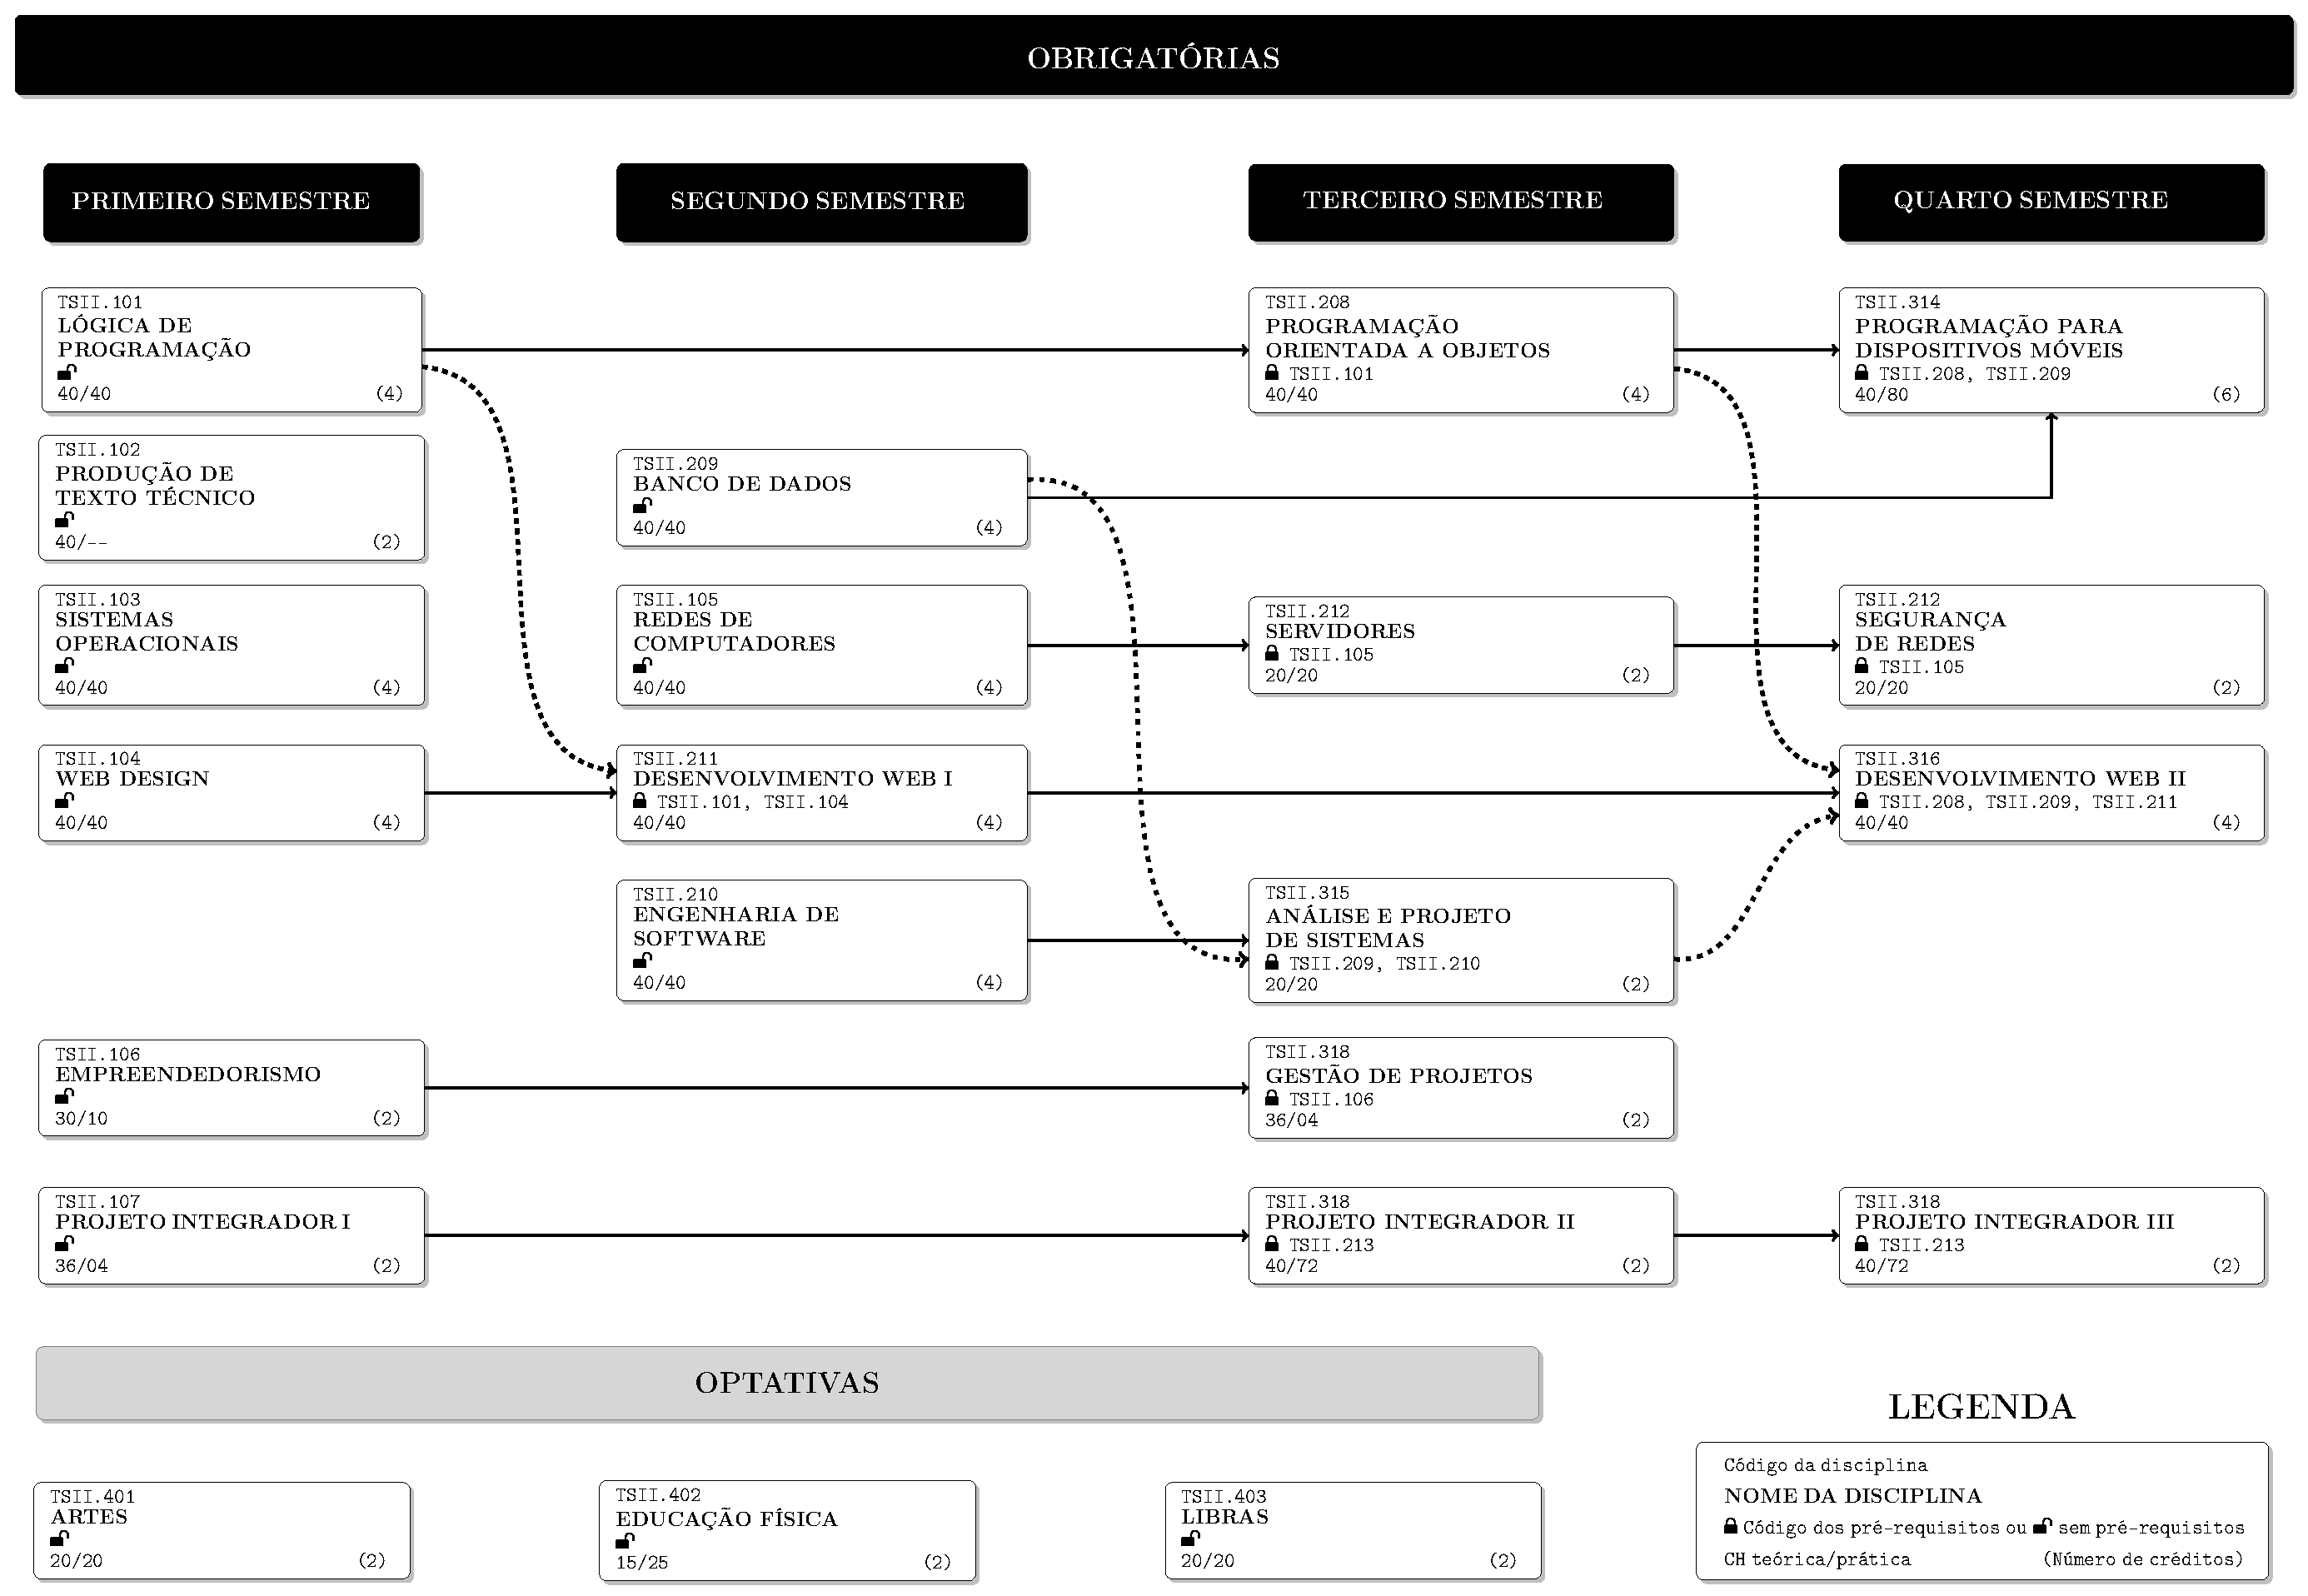
\includegraphics[width=\textwidth]{flow.pdf}
}{
    \fonte{Comissão de Elaboração do Projeto Pedagógico do Curso.}
   }
\end{figure}

\color{black}

\chapter{Avaliação da aprendizagem}

Entendendo que avaliar, no processo de ensino e aprendizagem, é o ato de acompanhar a construção do conhecimento do discente, a avaliação da aprendizagem pressupõe promover o aprendizado, favorecendo o progresso pessoal e a autonomia do educando, num processo global, sistemático e participativo.

A proposta pedagógica do curso prevê uma avaliação que, de forma articulada, assuma as funções diagnóstica, formativa e somativa. Tais pressupostos de avaliação são utilizados como princípios para a tomada de consciência das dificuldades, conquistas e possibilidades dos discentes, funcionando como um conjunto de atuações que tem a função de alimentar, sustentar e orientar a intervenção pedagógica.

A avaliação será processual e contínua, com a predominância dos aspectos qualitativos sobre os quantitativos e dos resultados parciais sobre os obtidos em provas finais, em conformidade com o artigo 24, inciso V, alínea a, da LDB 9.394/96. O processo de avaliação será orientado pelos objetivos definidos nos PUDs do curso, na perspectiva de contribuir incessantemente para a efetiva aprendizagem do aluno. A avaliação do desempenho acadêmico é feita por componente curricular, utilizando-se de estratégias formuladas de tal modo que o discente seja estimulado à prática da pesquisa, da reflexão, da criatividade e do autodesenvolvimento.


Considerando que o desenvolvimento de competências envolve conhecimentos, práticas e atitudes, o processo avaliativo exige diversidade de instrumentos e técnicas de avaliação, que deverão estar diretamente ligadas ao contexto da área objeto da educação profissional e utilizadas de acordo com a natureza do que está sendo avaliado.

Pensando numa conjugação de instrumentos que permitam captar melhor as diversas dimensões dos domínios da competência (habilidades, conhecimentos gerais, atitudes e conhecimentos técnicos específicos), o ROD do IFCE em seu art. 94. § 1$^\circ$, referenda alguns instrumentos e técnicas:

\begin{alineas}
\item  Observação diária dos estudantes pelos professores, durante a aplicação de suas diversas atividades;  
\item  Exercícios;
\item Trabalhos individuais e/ou coletivos;
\item Fichas de observações;
\item Relatórios;
\item Autoavaliação;
\item Provas escritas com ou sem consulta;
\item  Provas práticas e provas orais;
\item  Seminários;
\item  Projetos interdisciplinares;
\item Resolução de exercícios;
\item Planejamento e execução de experimentos ou projetos;
\item Relatórios referentes a trabalhos, experimentos ou visitas técnicas;
\item Realização de eventos ou atividades abertas à comunidade;
\item Autoavaliação descritiva e outros instrumentos de avaliação considerando o seu caráter progressivo. 

\end{alineas}

De acordo com o ROD, a sistemática de avaliação dos conhecimentos construídos, nos cursos com regime de crédito por disciplina, com periodicidade semestral, se desenvolverá em duas etapas. Devendo ser registrada no sistema acadêmico apenas uma nota para a primeira etapa (N1) e uma nota para a segunda etapa (N2), com pesos 2 e 3, respectivamente e, independentemente do número de aulas semanais, o docente deverá aplicar, no mínimo, duas avaliações em cada uma das etapas.

O cálculo da média parcial (MP) de cada disciplina ofertada semestralmente deve ser feito de acordo com a seguinte equação:
\[
    \mathrm{MP} = \frac{2 \times \mathrm{N1} + 3 \times \mathrm{N2}}{5}.
\]

Deverá ser considerado aprovado no componente curricular o estudante que, ao final do período letivo, tenha frequência igual ou superior a 75\% (setenta e cinco por cento) do total de horas letivas e tenha obtido média parcial (MP) igual ou superior a 6,0 (seis). 

O estudante aprovado com a nota da MP não precisará realizar a avaliação final (AF), e sua média final (MF) deverá ser igual a sua média parcial (MP). O estudante que obtiver MP inferior a 6,0 (seis) e maior ou igual a 3,0 (três) deverá fazer avaliação final (AF). A avaliação final deverá ser aplicada no mínimo 3 (três) dias letivos após o registro do resultado da MP no sistema acadêmico e poderá contemplar todo o conteúdo trabalhado no período letivo.

A nota da avaliação final (AF) deverá ser registrada no sistema acadêmico e, neste caso, o cálculo da média final (MF) deverá ser efetuado de acordo com a média aritmética simples entre a AF e a MP, como mostrado na seguinte equação:
\[
    \mathrm{MF} = \frac{ \mathrm{MP} + \mathrm{AF}}{2}.
\]

Deverá ser considerado aprovado na disciplina o estudante que, após a realização da avaliação final, obtiver média final (MF) igual ou maior que 5,0 (cinco).

Para aqueles discentes que não atingirem desempenho satisfatório, é garantido o direito à recuperação da aprendizagem como previsto na LDB e no ROD. Para tanto, a partir da primeira etapa, poderão ser realizadas ações institucionais, tais como:
\begin{alineas}
	\item a verificação da sistemática de avaliação ao longo das etapas e semestres do curso;
 	\item (re)orientação do processo educativo quando os resultados atingidos forem insatisfatórios diante dos objetivos esperados;
 	\item o desenvolvimento de turmas de apoio extraclasse, admitindo uma metodologia de ação, como as células de aprendizagem colaborativa;
 	\item o fortalecimento de políticas institucionais como a monitoria remunerada e voluntária para turmas com resultados insatisfatórios, inicialmente;
 	\item a colaboração e apoio ao trabalho docente diante das demandas contextuais e institucionais.
\end{alineas}



\chapter{Prática profissional Supervisionada - PPS}
% ADS
As atividades de Prática Profissional Supervisionada (PPS) estão previstas
com carga horária total de 40 (quarenta) horas. Elas são desenvolvidas nos
componentes curriculares de Ética e Responsabilidade Socioambiental, Empreendedorismo e Projeto Integrador Multidisciplinar.

Estas atividades têm por finalidade enriquecer a aprendizagem, privilegiando a
complementação da formação social e profissional dos discentes e a articulação
entre teoria e prática, além de colaborar para a elevação da qualidade
profissional dos discentes.

A prática profissional visa:
\begin{alineas}
	\item promover a integração teórica e prática dos conhecimentos, habilidades e
técnicas desenvolvidas no currículo;
	\item proporcionar situações de aprendizagem em que o estudante possa
interagir com a realidade do trabalho, reconstruindo o conhecimento pela
reflexão-ação complementar à formação profissional;
	\item desencadear ideias e atividades alternativas;
	\item atenuar o impacto da passagem da vida acadêmica para o mercado de
trabalho; e
	\item desenvolver e estimular as potencialidades individuais proporcionando o
surgimento de profissionais empreendedores, capazes de adotar modelos
de gestão e processos inovadores. 
	 	
\end{alineas}

Tais atividades estão integradas às disciplinas e objetivam a integração teoria-
prática, com base no princípio da interdisciplinaridade. Elas devem constituir-se em
um espaço de complementação, ampliação e aplicação dos conhecimentos adquiridos
durante o curso, tendo em vista a intervenção no mundo do trabalho e na realidade
social, além de contribuir para a solução de problemas, caso detectados.


A metodologia a ser adotada será através de visitas, estudos de caso,
atividades em laboratório, desenvolvimento de projetos, entre outras, com
levantamento de problemas relativos ao objeto da pesquisa e possíveis soluções para
os problemas detectados.

Mais especificamente, no componente  Projeto Integrador Multidisciplinar, configurar-se-á uma oportunidade na qual os alunos, por meio de uma produção acadêmica e/ou técnico-científica, a integração dos conhecimentos trabalhados durante o seu percurso formativo, de forma que se possa, ao final, demonstrar o resultado da experiência ensino-aprendizagem e o domínio de competências para o exercício de sua profissão.

A seguir, são elencados elementos norteadores para realização das atividades referentes ao Projeto Integrador Multidisciplinar:

\begin{alineas}
	\item Exploração das temáticas de educação das relações étnico-raciais, história e cultura afro-brasileira e indígena, bem como educação ambiental. Também deve trabalhar o desenvolvimento de projetos para resolução de problemas que envolvam as temáticas em questão de forma integradora, possibilitando  o desenvolvimento de uma visão dialógica e integrada  suas relações com a sociedade contemporânea;
	\item Aperfeiçoar o trabalho em equipe e desenvolver uma cultura solidária de partilha e de compromisso social, de modo que possam construir e exercitar a sua cidadania contribuindo para melhoria da qualidade de vida dos cidadãos envolvidos no projeto. Assim, espera-se que o projeto que vise atividades que contribuam para melhoria da qualidade de vida da sociedade local, principalmente em comunidades carentes, para o desenvolvimento sustentável, a valorização dos direitos humanos, a conscientização ambiental, a educação nas relações étnico-raciais e sua participação como cidadão compromissado com o bem-estar social. Todo este arcabouço de ideias devem contribuir para a execução de um projeto que construa e exercite a cidadania contribuindo para melhoria da qualidade de vida dos cidadãos envolvidos no projeto;
	\item Propiciar aos discentes o conhecimento teórico das competências, habilidades e atitudes empreendedoras e de inovação, ao passo que, de modo prático, introduz ao gerenciamento de projetos, análise de riscos e custos, gerenciamento da qualidade, liderança e trabalho em equipe, culminando na avaliação de resultados do projeto proposto.


\end{alineas}


\subsection{Monitoria}

É sabido que várias disciplinas do curso  requerem dos discentes  uma nova forma de se comunicar com o computador para instruí-lo a realizar operações. No entanto, é sabido também que dentro da formação regular, geralmente não há o ensino e aprendizagem desta  habilidade de comunicação e manipulação do computador,  levando os estudantes a terem grandes dificuldades e, consequentemente, apresentarem baixo rendimento durante o curso.

Diante da complexidade e novidade dos conte\'udos abordados no cursos e do  volume de atividades propostas para os discentes, justifica-se a presen\c{c}a de um discente monitor em algumas disciplinas que poder\'a contribuir de forma efetiva para a aprendizagem dos demais discentes. Tal a\c{c}\~ao, objetiva a melhoria de  desempenho dos discentes, al\'em de contribuir para a melhoria geral da qualidade das disciplinas e, consequentemente, do curso. 

Logo, tão cedo quanto possível,  os discentes do curso têm a oportunidade de, semestralmente, participarem do processo de seleção para atividades de monitoria nas disciplinas, com ou sem remuneração. O exercício de monitoria permite adquirir créditos na modalidade de atividades complementares.


\textbf{São atividades comum do Discente Monitor}:
\begin{alineas}
\item Auxiliar os demais alunos na resolução de exercícios;
\item Auxiliar os demais alunos no esclarecimento de dúvidas;
\item Auxiliar o professor nas discussões em sala de aula;
\item Auxiliar o professor a identificar dificuldades dos alunos na disciplina, com vistas ao melhor aproveitamento do conteúdo; e por fim,
\item Orientar os demais alunos acerca da pesquisa bibliográfica e do acervo existente na biblioteca objeto de estudo da disciplina.

\end{alineas}


\textbf{São atividades do Docente Orientador de Monitoria}:
\begin{alineas}
\item Orientar sistematicamente o monitor quanto à metodologia utilizada no atendimento aos demais alunos;
\item Auxiliar e supervisionar o monitor em sua atuação, quanto à elaboração dos relatórios e demais atividades; e por fim,
\item Acompanhar e avaliar o estudante monitor.
\end{alineas}

Dentre os possíveis resultados, destacam-se: 
\begin{alineas}
\item Um melhor aproveitamento do componente curricular, cujo conteúdo será utilizado em outras componentes no decorrer do curso;
\item Um nivelamento dos discentes quanto à aprendizagem; e por fim,
\item Uma maior participação dos discentes em sala de aula.
\end{alineas}



\chapter{Estágio supervisionado}

O estágio supervisionado não obrigatório poderá ser realizado em empresas de computação, informática, telecomunicações, escritórios de projetos e consultoria, empresas de montagem e manutenção de equipamentos eletrônicos, indústrias diversas, empresas comerciais de pequeno e grande porte, desde que ofereçam ambiente para a prática profissional da Informática.  Desenvolvidos nas modalidades tempo parcial ou tempo integral, os estágios devem ser supervisionados no local onde é ofertado, podendo ser realizados em períodos de férias ou durante os dias letivos, desde que não prejudiquem o desempenho do aluno nas disciplinas em que está matriculado.
Os estágios constituem oportunidade de aproximação do IFCE com a empresa, podendo resultar em parcerias, acordos de cooperação, convênios, consultorias e outras formas de parceria.


O estágio supervisionado poderá ainda ser realizado no âmbito do próprio IFCE, nos laboratórios do \textit{campus}, através de atividades de extensão ou projetos integradores ou bolsas de iniciação científica. Nesses casos, o estágio supervisionado será orientado por professor da instituição de ensino superior concedente, através de atividades correspondentes a uma carga horária didática semanal de no mínimo 12 horas até o máximo de 20 horas.

Antes do início do estágio supervisionado, a entidade concedente deverá firmar um termo de compromisso com o IFCE e com o estagiário e fazer um seguro de acidentes pessoais em benefício do estagiário, com ônus para a concedente conforme a lei de \nord{11.788}, de 25 de setembro de 2008. O início do estágio supervisionado deve ser precedido pela designação de um professor orientador no IFCE e pela elaboração de um plano de estágio, cujo acompanhamento será efetuado pelo orientador através de relatórios parciais, contatos com o supervisor de estágio na empresa, correio eletrônico, telefone, correspondência e, caso necessário, visitas ao local do estágio. Ao final do estágio, o aluno deverá elaborar um relatório final de estágio supervisionado, onde são detalhadas as atividades desenvolvidas. A avaliação do relatório final de estágio supervisionado será realizada pelo orientador de estágio, que emitirá seu parecer e nota. 

A realização do estágio nas férias não dispensa a designação prévia de um
professor orientador, a elaboração do plano de estágio, a assinatura do termo de compromisso e a contratação de um seguro de acidentes pessoais em favor do estagiário.

As atividades de estágio do IFCE \textit{campus} Tauá são geridas e acompanhadas pela Comissão de Coordenação de Estágio, conforme  \href{https://sei.ifce.edu.br/sei/controlador_externo.php?acao=documento_conferir&codigo_verificador=5049721&codigo_crc=D2A855C5&hash_download=8211d5eecb230cb8765ceb54199b56b9dcf61d684050d5c575df55732d493c4e40f77568847d43c092af63a30df085c55666384493a581b4cc78038b5247d885&visualizacao=1&id_orgao_acesso_externo=0}{PORTARIA \nord{176}/GAB-TAU/DG-TAU/TAUA, DE 29 DE JUNHO DE 2023}. Destaca-se, ainda, que é papel do corpo docente do Curso Técnico de Informática para Internet discutir e avaliar continuamente a política de estágios do curso, promovendo aperfeiçoamentos necessários à sua execução, acompanhando e avaliando a sua operação.


\subsection{Atividades de Pesquisa e Extensão}
Os alunos do curso são incentivados a participarem de projetos de pesquisa e extensão junto aos docentes do curso. Esses projetos podem estar vinculados a uma bolsa de pesquisa de iniciação científica dos programas de pesquisa regidos por editais do IFCE, como o  Programa Institucional de Bolsas de Iniciação Científica Júnior (PIBIC Jr.), a projetos integradores, a programas de pesquisa próprios do \textit{campus} Tauá, entre outros. 


\chapter{Critérios de aproveitamento de conhecimentos e experiências anteriores}


É assegurado ao discente do IFCE o direito de aproveitamento de componentes curriculares cursadas em outros cursos técnicos de nível médio reconhecidos pelo MEC ou a validação de conhecimentos como forma de aproveitamento de conhecimentos e experiências. Este aproveitamento dá-se mediante análise da compatibilidade de conteúdo e da carga horária, no mínimo 75\% (setenta e cinco por cento) do total estipulado para o componente curricular.

O discente poderá solicitar aproveitamento de componentes curriculares, mediante apresentação de requerimento protocolado e enviado à coordenadoria do curso acompanhado de histórico escolar e dos Programas de Unidades Didáticas e/ou ementas, devidamente autenticados pela instituição de origem.

O prazo para a solicitação do aproveitamento de componentes curriculares será:
\begin{alineas}
\item Alunos novatos: nos 10 primeiros dias logo após a matrícula;
\item  Alunos veteranos: primeiros 50 (cinquenta) dias letivos do semestre em curso.
\end{alineas} 

Ao discente também será permitida a validação de conhecimentos adquiridos em estudos regulares ou em experiência profissional, mediante avaliação teórica e/ou prática, feita por uma banca instituída pelo gestor máximo do ensino no \textit{campus}, composta, no mínimo, de dois professores. 

De acordo com art. 140 do ROD, a solicitação de validação de conhecimentos deverá ser feita mediante requerimento protocolado e enviado à coordenadoria do curso, junto com o envio dos seguintes documentos: 
\begin{itemize}
\item[]
\begin{itemize}
	\item [I.] declaração, certificado ou diploma - para fins de validação em conhecimentos adquiridos em estudos regulares; 
	\item [II.] cópia da Carteira de Trabalho (páginas já preenchidas) ou declaração do empregador ou de próprio punho, quando autônomo - para fins de validação de conhecimentos adquiridos em experiências profissionais anteriores. 
\end{itemize}
\end{itemize}

Ainda de acordo com o ROD, a validação de conhecimentos deverá ser solicitada nos primeiros 30 (trinta) dias do período letivo em curso e todo o processo de validação deverá ser concluído em até 50 (cinquenta) dias letivos do semestre vigente, a contar da data da solicitação do estudante. 


\chapter{Emissão de diploma}

Após a integralização dos componentes curriculares previstos para o Curso Técnico Subsequente em Informática para Internet e a conclusão da carga horária prevista para a prática profissional, será expedido ao concluinte o diploma de Técnico em Informática para Internet. Os diplomas deverão ser acompanhados do Histórico Escolar em que constem todos os componentes curriculares cursados, com suas respectivas cargas horárias, frequências e aproveitamento dos discentes. O modelo do diploma seguirá a legislação vigente e o modelo utilizado pelo IFCE.


\chapter{Avaliação do projeto do curso}


O processo de avaliação do curso acontecerá através de reuniões periódicas entre professores, Coordenador do curso e Coordenação Técnico Pedagógica e de reuniões do Colegiado do curso, nas quais se discute assuntos relacionados ao bom andamento das atividades, tais como: indicadores de aprendizagem, políticas de melhoria que garantam maior eficácia no processo ensino-aprendizagem e melhoria na infraestrutura do curso como um todo, além de um efetivo acompanhamento ao aluno egresso.

A avaliação será realizada ainda com base no levantamento de uma variedade de indicadores de desempenho da Instituição, cujos resultados podem subsidiar o dimensionamento do nível de satisfação dos docentes e discentes com o trabalho e envolvimento no âmbito do Curso, resultando em ações desencadeadas no Plano de Desenvolvimento Institucional (PDI) e também no Plano de Ação Anual (PAA) da Instituição.

Nesse sentido, o \textit{campus} Tauá adota os seguintes instrumentais de avaliação:
\begin{alineas}
		\item \textbf{Avaliação docente} - feita por meio de um questionário no qual os alunos respondem questões referentes à conduta docente, atribuindo notas de 1 (um) a 5 (cinco), relacionadas à pontualidade, assiduidade, domínio de conteúdo, incentivo à participação do aluno, metodologia de ensino, relação professor-aluno e metodologia de avaliação.  No mesmo questionário os alunos avaliam o desempenho dos docentes quanto a pontos positivos e negativos e apresentam sugestões para a melhoria do Curso e da Instituição. Os resultados são apresentados aos professores com o objetivo de contribuir para a melhoria das ações didático-pedagógicas e da aprendizagem discente.
	\item \textbf{Avaliação Institucional} - a Comissão Própria de Avaliação (CPA) realiza diagnóstico das condições das instalações físicas, equipamentos, acervos e qualidade dos espaços de trabalho do Instituto e encaminha aos órgãos competentes relatório constando as potencialidades e fragilidades da instituição, para conhecimento e possíveis soluções.

\end{alineas}

O Colegiado do Curso supervisiona as atividades curriculares, propondo/aprovando e avaliando reestruturações no projeto pedagógico do curso, bem como cuidando de questões didáticas pedagógicas que perfazem as ações docentes e discentes na instituição. Além disso, o Colegiado colabora com decisões acerca do desenvolvimento do curso e daqueles que dele fazem parte, viabilizando projeções de melhoria e viabilidade do projeto pedagógico.

A Direção Geral, o Departamento de Ensino, o Departamento de Administração e Planejamento e a Coordenação do Curso subsidiarão as instâncias envolvidas no processo de avaliação do projeto do curso.

Este PPC será analisado pelo menos uma vez a cada ano e meio (ciclo de uma turma) tendo em vista a oferta e demanda, 
demonstradas pela clientela com possíveis mudanças estruturais e pedagógicas. Além disso, os ganhos estruturais do \textit{campus}, em termos de novos espaços, acervos de equipamentos e bibliográficos, também devem indicar adequações do PPC.

\chapter{Atuação do coordenador do curso}

A Coordenação do Curso Técnico em Informática para Internet atua para promover o sucesso das ações acadêmicas e administrativas no
âmbito do curso, estabelecendo o diálogo entre estudantes, professores e demais
membros da equipe gestora.

As atribuições do coordenador do curso estão definidas na Nota Técnica \nord{2}
PROEN, de 18 de maio de 2015. O coordenador do curso também atua de acordo
com um plano de ação, cujo procedimento de elaboração é definido na Nota Técnica
\nord{4} PROEN, de 30 de novembro de 2018.


\chapter{Políticas Institucionais Constantes do PDI}% no Âmbito do Curso}


O modelo de planejamento estratégico do IFCE para o quinquênio
2024-2028, do Plano de Desenvolvimento Institucional~\footnote{Disponível em:
\url{https://pdi.ifce.edu.br/pdf/pdi_ifce_2024_2028.pdf}}, buscou dar ênfase aos macroprocessos da cadeia de valor da instituição,
assegurando que as tomadas de decisões estejam voltadas para a geração de valor
para a sociedade. Assim, para esta edição do PDI (2024-2028), ao invés de estabelecer indicadores próprios, optou-se
por utilizar os indicadores que foram estabelecidos pela Setec para monitorar o
desempenho da Rede Federal de Educação Profissional, Científica e Tecnológica
(RFEPCT)\footnote{\href{https://www.in.gov.br/en/web/dou/-/portaria-n-299-de-6-de-maio-de-2022-399680297}{Portaria \nord{299}, de 06 de maio de 2022}
que dispõe sobre os indicadores de Pesquisa e Extensão a serem utilizados pelas
Instituições que compõem a Rede Federal de Educação Profissional, Científica e
Tecnol\'ogica (Rede Federal de EPCT).}.


Essa abordagem traz consigo uma série de vantagens, assegurando ainda que a
instituição esteja em conformidade com as diretrizes e políticas nacionais
estabelecidas para a RFEPCT. Com a mudança, as metas  referem-se a algo que pode ser medido ou expresso numericamente. Elas são
associadas aos indicadores de desempenho e são critérios de avaliação de desempenho da instituição.

Na listagem abaixo  são elencadas as metas que o  Curso Técnico Subsequente em
Informática para Internet oportunizará dentro do PDI 2024-2028:
\begin{alineas}
\item \textbf{ENS-1}. 
Matrículas em cursos
técnicos;
	\item \textbf{P\&I-1}.
Porcentagem de projetos
de pesquisa aplicada;
\item \textbf{P\&I-4}.
Porcentagem de alunos
provenientes das ações
afirmativa da instituição
envolvidos em projetos de
pesquisa. 
	\item \textbf{P\&I-3}. Porcentagem de alunos da
instituição envolvidos em
projetos de pesquisa;
\item \textbf{EXT-1}.
Percentual de recursos
financeiros do orçamento
anual público aplicados em
extensão; e 
	\item  \textbf{EXT-3}.
Percentual de servidores
envolvidos em ações de
extensão.
\end{alineas}

Ademais, são elencadas as metas que o Curso Técnico Subsequente em Informática
para Internet oportunizará dentro do Plano de Desenvolvimento Institucional do
\textit{campus} Tauá.

\textbf{No âmbito do Ensino}:

	\begin{alineas}
	  \item Ampliação do número de estudantes egressos com êxito;
	  \item Sedimentar ações de realização de seminário ou fórum de educação profissional de nível técnico do IFCE;
	  \item Ampliar o índice Relação Aluno -- professor;
	  \item Realização de feiras científicas e tecnológicas e olimpíadas internas e externas.
	\end{alineas}
	
	\textbf{Pesquisa, Inovação e Pós-graduação}:
	\begin{alineas}
	  \item Expandir e consolidar a inovação: Volume de recursos captados em projetos de Pesquisa e Desenvolvimento; e Depósitos de propriedade intelectual;
	  \item Ampliar a parceria com empresas, instituições diversas para captação de projetos. Ampliar as parcerias e o volume de recursos captados em projetos de PD\&I;
	  \item Mapear o potencial de inovação do campus;
	  \item Expandir e consolidar a pesquisa científica institucional, através de uma média de 02 (duas) produções anuais por pesquisador cadastrado na plataforma NL da PRPI;
	  \item Estimular, nas pessoas residentes nas regiões visitadas pelo campus, o gosto e a curiosidade pelas ciências e artes, bem como apresentar as áreas do conhecimento ofertadas no campus e as formas de interação do campus com a sociedade (Extensão-Pesquisa-Ensino).
	\end{alineas}
	
	\textbf{Extensão}:
	\begin{alineas}
	  \item Fortalecer as relações socioprodutivas e culturais nos contextos locais e regionais através do aumento da taxa de discentes matriculados em estágio curricular;
	  \item Realizar momentos de integração entre empresas públicas, privadas e o campus, aumen- tando a quantidade e qualidade das ofertas de estágio;
	  \item Aumentar o número de empresas com convênio de estágio devidamente celebrado, visando ampliar o número de vagas de estágio em empresas parceiras;
		\item Ampliar as parcerias com ecossistemas empreendedores em âmbito local, estadual e nacional, visando aumento da taxa de parcerias em ações de empreendedorismo.
	  

	\end{alineas}


\chapter{Apoio ao discente}
O IFCE \textit{campus} Tauá possibilita aos estudantes algumas ações estratégicas de apoio através dos setores de Assistência Estudantil, Coordenação Técnico-Pedagógica e das demais atividades relacionadas ao desenvolvimento integral do educando.


\section{Assistência Estudantil}
O  Setor de Assistência Estudantil que tem por finalidade a ampliação das condições de permanência dos jovens na educação pública federal pauta-se nos objetivos estabelecidos no Programa Nacional de Assistência Estudantil (Decreto 7.234/2010), a saber:
\begin{itemize}
\item[]
\begin{itemize}
    \setlength\itemsep{0em}
    \item[I -] democratizar as condições de permanência dos jovens na educação superior pública federal;
    \item[II -] minimizar os efeitos das desigualdades sociais e regionais na permanência e conclusão da educação superior;
    \item[III -] reduzir as taxas de retenção e evasão; e
    \item[IV -] contribuir para a promoção da inclusão social pela educação.
\end{itemize}
\end{itemize}

O setor poderá ser composto por uma equipe multidisciplinar: assistente social, psicólogo,
enfermeira, odontólogo, nutricionista e técnica em enfermagem. As ações da assistência estudantil possuem dois eixos norteadores: o primeiro com os serviços que visam atender a toda comunidade discente com o atendimento biopsicossocial; e o segundo, com os auxílios que se destinam ao atendimento prioritário do discente em situação de vulnerabilidade social.


O IFCE concede as seguintes modalidades de auxílios: moradia; alimentação; transporte; óculos; visitas e viagens técnicas; acadêmico; didático-pedagógico; discentes mães/pais; formação; de apoio à cultura e ao desporto e pré-embarque internacional.

O serviço social atua no âmbito das relações sociais junto aos indivíduos, famílias, grupos, comunidades e movimentos sociais, desenvolvendo ações de fortalecimento da autonomia, da participação e do exercício da cidadania. Nesse sentido, o serviço de Psicologia objetiva contribuir para os processos de educação, saúde e bem-estar dos alunos e das pessoas, direta e indiretamente, ligadas ao contexto educacional do discente.

Os serviços de saúde também estão inseridos na Assistência Estudantil, desenvolvendo ações de prevenção, promoção e acompanhamento da saúde do discente, visando garantir, através de suas atividades, a permanência do mesmo na instituição e o direito à educação.

O serviço de alimentação e nutrição proporciona uma alimentação adequada e saudável, contribuindo para a promoção de hábitos alimentares saudáveis e favorecendo a permanência do estudante no espaço educacional.

A atuação em comum de todos os profissionais que integram o setor voltado para a assistência ao educando envolve a realização de diversas ações, a saber: atendimentos individuais; acolhida; orientações gerais e de grupos operativos e socioeducativos.

\section{Coordenadoria Técnico Pedagógica}
A Coordenadoria Técnico-Pedagógica (CTP) é responsável por promover, em parceria com os diversos setores da Instituição, ações que visem garantir o êxito do processo de ensino-aprendizagem. Tem por finalidade assessorar as atividades de ensino, pesquisa e extensão, supervisionando e avaliando estas atividades, para assegurar a regularidade do desenvolvimento do processo educativo.


\section{Coordenadoria de Controle Acadêmico}
A Coordenadoria de Controle Acadêmico (CCA) atua como setor de execução de processos e atendimento de demandas relacionadas ao Sistema Q-Acadêmico. No organograma institucional, está subordinada à Diretoria de Ensino. As principais atribuições deste setor estão voltadas para as atividades de ingresso, matrícula, criação de turmas, horários, expedição de diplomas dos cursos técnicos e demais documentos referentes à rotina acadêmica discente.

Os procedimentos realizados são pautados no ROD, que traz orientações sobre os princípios legais para as tomadas de decisão, respeitando as diretrizes previstas na legislação educacional vigente.


\section{Coordenação de Curso}

A Coordenação do Curso Subsequente em Informática para Internet atua para promover o sucesso das ações acadêmicas e administrativas no âmbito do curso, estabelecendo o diálogo entre estudantes, professores e demais membros da equipe gestora.

As atribuições do coordenador do curso estão definidas na Nota Técnica \nord{2} PROEN, de 18 de maio de 2015. O coordenador do curso também atua de acordo com um plano de ação, cujo procedimento de elaboração é definido na Nota Técnica \nord{4} PROEN, de 30 de novembro de 2018.


\chapter{Corpo docente}


Detalhes do perfil docente necessário para o desenvolvimento do Curso Técnico Subsequente em Informática para Internet  estão descritos no \autoref{tab:perfil_docente},  incluindo a área e subárea de atuação, a quantidade de profissionais e as disciplinas relativas a esse segmento.



\begin{quadro}[htpb]
\IBGEtab{
   \caption{Perfil do docente necessário para a realização do curso.}
    \label{tab:perfil_docente}
}{
    % Please add the following required packages to your document preamble:
% \usepackage[table,xcdraw]{xcolor}
% Beamer presentation requires \usepackage{colortbl} instead of \usepackage[table,xcdraw]{xcolor}

\begin{tabular}{ p{11em} p{8em} p{1cm} p{6.5cm}}
\rowcolor[HTML]{000000} 
{\color[HTML]{FFFFFF}\textbf{Área}} &
  {\color[HTML]{FFFFFF}\textbf{Subárea}} &
  {\color[HTML]{FFFFFF}\textbf{QTD.}} &
  {\color[HTML]{FFFFFF}\textbf{Componentes curriculares}} \\
\rowcolor[HTML]{EFEFEF} 
Administração &
  Administração \newline de Empresas &
  1 &
  Empreendedorismo; \newline Gestão de Negócios; e \newline Ética e Responsabilidade Socioambiental. \\[2em]
Ciência da Computação &
  Sistemas \newline de  Computação &
  1 &
  Introdução à Computação; \newline Redes de Computadores; e \newline Desenvolvimento e Operações. \\[2em]
\rowcolor[HTML]{EFEFEF} 
Ciência da Computação &
  Metodologia e \newline Técnicas \newline da Computação &
  2 &
  Análise e Projeto de Sistemas; \newline Engenharia de Software; \newline Tecnologias WEB; e \newline  Testes e Qualidade de Software. \\[2em]
Ciência da Computação &
  Metodologia e \newline  Técnicas \newline da Computação \newline \textbf{OU} \newline Teoria da \newline Computação &
  2 &
  Banco de Dados; \newline Estrutura de Dados; \newline  Lógica de Programação; \newline Projeto Integrador Multidisciplinar; \newline  Programação Orientada a Objetos; e \newline Programação para Dispositivos Móveis. \\[2em]
\rowcolor[HTML]{EFEFEF} 
Letras &
  Língua Inglesa &
  1 &
  Inglês Técnico
\end{tabular}
   }{
    \fonte{Comissão de Elaboração do Projeto Pedagógico do Curso.}
            \vspace{-1em}
   }
\end{quadro}
Já o corpo docente do IFCE \textit{campus} Tauá que atuará durante o semestre
letivo 2024.2 no Curso  Técnico Subsequente em Informática para Internet está
descrito no \autoref{tab:corpo_docente}. No momento, atuarão no curso 07
professores, sendo que 03 possuem título de doutor (43\%) e  04 (57\%) possuem título de mestre.

O corpo docente do Curso Técnico Subsequente em Informática para Internet é formado por equipe experiente de professores com perfil profissional e acadêmico, que possuem tanto experiência no mercado na área de tecnologia quanto bagagem em pesquisas científicas na área de Computação. Em termos de regime de trabalho, todos dedicam-se exclusivamente ao IFCE. Logo, comprova-se, pelo corpo docente, tanto a qualificação técnica quanto à disponibilidade para dar suporte a um curso de bom nível acadêmico.


\begin{quadro}[h]
	\IBGEtab{
		\caption{Corpo docente existente no IFCE \textit{campus} Tauá.}
		\label{tab:corpo_docente}
	}{
	\small
\noindent\begin{tabularx}{\textwidth}{ X X X } 

	\toprule

	\doc{Adriana Merly Farias}{Mestra  em Letras}{Graduação em Letras -- Português e Inglês}{Língua Inglesa}
	
	\doc{Alan Medeiros Casteluber}{Doutor em Letras}{Graduação em Letras -- Português e Inglês}{Língua Inglesa}

	\doc{Amarilton Lopes Magalhães}{Mestre em Engenharia de Telecomunicações}{Graduação em Engenharia de Telecomunicações}{Sistemas de Telecomunicações}
	
	\doc{Anelise Daniela Schinaider}{Doutora em Agronegócios}{Graduação em Administração}{Administração} 
        
    \doc{Antônio Bruno Sales Dias}{Mestre em Letras}{Graduação em Letras Inglês}{Língua Inglesa}
    
    \doc{Antônio Sávio Silva Oliveira}{Mestre em Engenharia de Telecomunicações}{Graduação em Tecnologia em Telemática}{Sistemas de Telecomunicações}
        
	\doc{Carlos Getúlio de Freitas Maia}{Mestre Filosofia}{Graduação em Filosofia}{Filosofia}
	


\end{tabularx}

  }{}
\end{quadro}


\begin{quadro}[h]
	\IBGEtab{}{
	\small
\noindent\begin{tabularx}{\textwidth}{ X X X } 
    \doc{Cledinaldo Alves Pinheiro Junior }{Mestre em Música}{Graduação em Licenciatura em Música}{Cordas Dedilhadas} 

    \doc{Daniel de Sá Rodrigues}{Mestre em Letras}{Graduação em Letras Inglês}{Língua Inglesa}

	     \doc{Edson Alencar Collares de Bessa}{Mestre em Antropologia}{Graduação em Ciências Sociais}{Sociologia Geral}
         
   
            \doc{Elpida Andreia de Queiroz Niko Kavouras}{Mestra em Desenvolvimento e Meio Ambiente }{Graduação em Ciências Biológicas}{Biologia Geral}
            
            \doc{Erico Castro de Albuquerque Melo}{Mestre em Engenharia Elétrica}{Graduação em Engenharia Elétrica}{Sistemas de Telecomunicações}
            
            \doc{Gabriela Ismerim Lacerda}{Mestra  em Literatura Brasileira}{Graduação em Licenciatura em Letras Português e Inglês}{Língua Portuguesa}

          \doc{Jayme Félix Xavier Júnior }{Mestre em Educação Física}{Licenciatura em Educação Física}{Educação Física}
                   
            


	\end{tabularx}

  }{}
\end{quadro}

\begin{quadro}[h]
	\IBGEtab{}{
	\small

\noindent\begin{tabularx}{\textwidth}{ X X X } 

                   
            \doc{Jéssica Nunes Caldeira Cunha}{Mestra em Estudos Linguísticos}{Graduação em Letras -- Português e Inglês}{Língua Inglesa}
          
               \doc{Jhonata da Costa Bezerra}{Mestre em Matemática}{Graduação em Matemática}{Matemática Básica}
     
     			\doc{João Paulo Lima Cunha}{Doutor em Letras}{Graduação em Letras -- Português}{Língua Portuguesa}
     			
     			\doc{João Paulo Saraiva Pires}{Especialista em Docência do Ensino Superior}{Graduação em Pedagogia}{Currículo e Estudos Aplicados ao Ensino e Aprendizagem}
             
    	      \doc{José Alves de Oliveira Neto}{Mestre em Matemática}{Graduação em Matemática}{Matemática Básica}
    	      
    	      \doc{Julio Serafim Martins}{Mestre em Computação}{Graduação em Engenharia de Software}{Metodologia e Técnicas em Computação}
    	      
    	      \doc{Karina de Morais e Silva}{Mestra em Letras}{Graduação em Letras -- Língua Portuguesa}{Língua Portuguesa}

                     
         
\end{tabularx}

	  }{}
\end{quadro}



\begin{quadro}[h]
	\IBGEtab{}{
	\small

	\noindent\begin{tabularx}{\textwidth}{ X X X } 

                \doc{Kélvia Jacome de Castro}{Doutora em Zootecnia}{Graduação em Zootecnia}{Zootecnia}
                
                \doc{Kleiane Bezerra de Sá}{Doutora em Linguística}{Graduação em Letras-Português}{Língua Portuguesa}
                      
	  	\doc{Lucas Ferreira Mendes}{Mestre em Computação}{Graduação em Tecnologia em Telemática}{Sistemas de Computação}
         
         \doc{Marcelo Henrique de Araujo Santos Costa}{Doutor em Física}{Graduação em Física}{Física Experimental}
         
         \doc{Marcus Vinícius de Paula}{Mestre em Linguística Aplicada}{Graduação em Letras}{Língua Portuguesa}
         
         \doc{Marinaldo de Almeida Cunha}{Doutor em Educação}{Graduação em Pedagogia}{Currículo e Estudos Aplicados ao Ensino e Aprendizagem}
         
         
         \doc{Marselle Marmo do Nascimento Silva}{Doutora em Ciência dos Alimentos}{Graduação em Engenharia de Alimentos}{Tecnologia de Alimentos}
         
         
         
         
       
	\end{tabularx}

	  }{}
\end{quadro}




\begin{quadro}[h]
	\IBGEtab{}{
	\small

	\noindent\begin{tabularx}{\textwidth}{ X X X } 

             \doc{Nádia de Melo Braz}{Doutora em Zootecnia}{Graduação em Zootecnia}{Zootecnia}
             
             \doc{Nicomedes Albuquerque Pontes}{Mestre em Matemática}{Graduação em Licenciatura em Matemática}{Matemática Básica}
         
         \doc{Paulo Ricardo Barboza Gomes}{Doutor em Engenharia de Teleinformática}{Graduação em Engenharia de Telecomunicações}{Sistemas de Telecomunicações}
         
       
       	\doc{Phyllipe do Carmo Félix}{Especialista em Engenharia de Software}{Licenciatura em Computação}{Sistemas de Computação}
          
          \doc{Rafaela de Carvalho Baptista}{Doutora em Ciência de Alimentos}{Graduação em Engenharia de Alimentos}{Tecnologia em Alimentos}
          
          \doc{Raquel Vieira Sobrinho}{Mestra em Lingüística}{Graduação em Letras Português-Inglês}{Língua Portuguesa}
         		
         		\doc{Reginaldo Pereira Fernandes Ribeiro}{Especialista em Engenharia de Sistemas}{Graduação em Licenciatura em Computação}{Metodologia e Técnicas da Computação}
         
       
	\end{tabularx}

	  }{}
\end{quadro}


\newpage


\begin{quadro}[t]
	\IBGEtab{
		\vspace{2em}
	}{
	\small

	\noindent\begin{tabularx}{\textwidth}{ X X X } 

         
          \doc{Roberto Luís Alexandrino Feitosa }{Mestre em Engenharia Civil}{Graduação em Engenharia Química}{Química Geral}
          
       

        \doc{Samuel Alves Soares}{Mestre em Ciências da Computação}{Graduação em Ciências da Computação}{Metodologia e Técnicas  da Computação}
        
        \doc{Samuel Barbosa Silva}{Doutor em Linguística}{Graduação em Letras}{Língua Portuguesa} 
         
        \doc{Saulo Anderson Freitas de Oliveira}{Doutor em Ciência da Computação}{Graduação em Ciência da Computação}{Metodologia e Técnicas  da  Computação}
        
        \doc{Tiago de Sousa Leite}{Doutor em Fitotecnia}{Graduação em Agronomia}{Fitotecnia}
    	
        \doc{Weberte Alan Sombra}{Mestre em Engenharia Agrícola}{Graduação em Agronomia}{Pastagem e Forragicultura}

        \doc{Willame de Araújo Cavalcante}{Mestre em Engenharia Hidráulica e Saneamento}{Graduação em Ciências Ambientais}{Gestão Ambiental}
          

       	\bottomrule
	\end{tabularx}

	  }{
	  	\fonte{Comissão de Elaboração do Projeto Pedagógico do Curso.}

		\vspace{40em}

	  }
\end{quadro}


\chapter{Corpo técnico-administrativo}
O  corpo técnico-administrativo relacionado ao curso está descrito no \autoref{tab:corpo_tae}.

%%%% TECNICOS
\begin{quadro}[h]
\IBGEtab{
    \caption{Corpo Técnico-Administrativo do \textit{campus} Tauá.}
    \label{tab:corpo_tae}
}{
	\small
\noindent\begin{tabularx}{\textwidth}{ XX } 
    \toprule      
    
    \tecn{Alex Modolo}{Programador Visual}{Graduação}{Comunicação Social} 
    
    
    \tecn{Alexciano de Sousa Martins}{Técnico em Assuntos Educacionais}{Mestrado}{Coordenação Técnico-Pedagógica} 
    
    \tecn{Aline Santos de Lima}{Auxiliar em Administração}{Especialização}{Gabinete do Diretor Geral}
    
     \tecn{Alisson Bezerra Silva}{Assistente em Administração}{Graduação}{Coordenadoria de Controle Acadêmico} 
    
    
    \tecn{Analice Fraga de Oliveira }{Bibliotecária}{Graduação}{Biblioteca} 
    
     \tecn{André Luíz de Araújo Barros}{Auxiliar de Biblioteca}{Ensino Médio}{Biblioteca} 
    
    \tecn{Carlos André Monteiro de Sousa}{Contador}{Graduação}{Departamento de Administração e Planejamento}
   
    \tecn{Claudenira Cavalcante Melo}{Assistente Social}{Mestrado}{Assistência Estudantil} 
    

    \tecn{Denis Rafael Pires Ferreira}{Auxiliar em Administração}{Especialização}{Coordenadoria de Controle Acadêmico}
    
   
\end{tabularx}
}{
}
\end{quadro}

\begin{quadro}[h]
	\IBGEtab{}{
		
		\small
		\noindent\begin{tabularx}{\textwidth}{ XX } 
                			
                    \tecn{Edmarcos Rodrigues Gonçalves}{Assistente em Administração}{Ensino Médio}{Coordenadoria de Aquisições e Contratações}    
    
    \tecn{Fábio Reis de Vasconcelos}{Tecnólogo--Formação}{Graduação}{Coordenadoria de TI} 
     
     \tecn{Francisca Paula Araujo de Sousa}{Assistente em Administração}{Ensino Médio}{Departamento de Administração e Planejamento}
   
    \tecn{George Luíz de Freitas Souza}{Assistente em Administração}{Especialização}{Departamento de Administração e Planejamento} 
    
                    
                    \tecn{Gessianne Carvalho Castro}{Assistente em Administração}{Especialização}{Coordenadoria de Controle Acadêmico} 
                    
                    \tecn{Jackson Weslley do Nascimento}{Administrador}{Especialização}{Infraestrutura} 
                    
                      \tecn{Janiele Vital Norões}{Assistente em Administração}{Especialização}{Gabinete do Diretor Geral} 
                    
                    \tecn{Jardel Leite de Oliveira}{Técnico em Laborátorio em Física}{Especialização}{Laboratório de Física} 
                        \tecn{João Paulo Oliveira}{Técnico de Tecnologia da Informação}{Especialização}{Coordenadoria de TI} 

		  \tecn{José Orlando dos Santos Lopes}{Assistente de Alunos}{Especialização}{Coordenadoria Técnico-Pedagógica } 

                    
                    \tecn{Jobson Vital Costa }{Psicólogo}{Mestre}{Assistência Estudantil} 
                    
               		
		\end{tabularx}
	
	}{}
\end{quadro}


\begin{quadro}[h]
	\IBGEtab{}{
		
		\small
		\noindent\begin{tabularx}{\textwidth}{ XX } 
		
		      
                    
                    \tecn{José Wendell Araujo Pedrosa }{Auxiliar em Biblioteca}{Ensino Médio}{Biblioteca} 
                
                
                    \tecn{Juliana Cândida Albano }{Técnica em Audiovisual}{Graduação}{Comunicação Social} 
                    
                   	              



		  \tecn{Juliana Sousa Rodrigues}{Assistente de Alunos}{Graduação}{Coordenadoria Técnico-Pedagógica} 
                
    
        


                       \tecn{Karla Gonçalves de Oliveira }{Pedagoga}{Especialização}{Coordenadoria Técnico-Pedagógica} 
                    

        \tecn{Lorene Maciel Barreto}{Técnico em Secretariado}{Especialização}{Administração} 

    \tecn{Marcus Vinícius de Moura Pacheco}{Técnico de Tecnologia da Informação}{Graduação}{Coordenadoria de TI} 


    \tecn{Margarida Maria Xavier da Silva}{Técnica em Laboratório de Biologia}{Mestrado}{Laboratório de Biologia} 
    
    
    \tecn{Maria Erivalda Costa de Oliveira}{Técnica em Secretariado}{Especialização}{Departamento de Ensino} 
    
    	\tecn{Meiryfrance Cavalcante Vital}{Assistente em Administração}{Especialização}{Administração} 
	
	      	\tecn{Micaelle de Oliveira Vieira}{Nutricionista}{Especialização}{Assistência Estudantil} 

        \tecn{Prucina de Carvalho Bezerra}{Pedagoga}{Mestrado}{Coordenadoria Técnico-Pedagógica} 

   	\end{tabularx}
	
	}{
	}
\end{quadro} 
    
    \clearpage
    
\begin{quadro}[t]
	\IBGEtab{}{
		
		\small
		\noindent\begin{tabularx}{\textwidth}{ XX } 
		
    \tecn{Rafael Eferson Pinheiro Nogueira}{Técnico em Eletrotécnica}{Graduação}{Infraestrutura} 
    
		\tecn{Rogério Barbosa de Araujo dos Santos}{Assistente em Administração}{Especialização}{Infraestrutura}


       \tecn{Sharlene Pereira Alves}{Enfermeira}{Graduação}{Assistência Estudantil} 
    
    \tecn{Stephanie de Oliveira Figueiredo }{Tecnólogo-Área Gestão de RH}{Graduação}{Coordenadoria de Gestão de Pessoas}
		
		
		
		\end{tabularx}
	
	}{
		\fonte{Comissão de Elaboração do Projeto Pedagógico do Curso.}
	}

\end{quadro}
	\vspace{10em}
\ 

\chapter{Infraestrutura}

O IFCE \textit{campus} Tauá conta com vários espaços de apoio ao discente,
podendo destacar: uma quadra esportiva coberta, um refeitório, uma biblioteca, laboratórios de apoio pedagógico e salas de aula amplas e arejadas.

A acessibilidade às Pessoas com Deficiência (PcD) demanda adaptações arquitetônicas e pedagógicas específicas. Em relação à estrutura arquitetônica, o  \textit{campus}  Tauá dispõe, em suas instalações, de rampas que possibilitam o acesso a todos os setores do pavimento térreo, bem como a todos os ambientes do pavimento superior.

Em relação à estrutura pedagógica, conforme a diversidade da demanda, o curso se utilizará dos diversos recursos que garantam as condições necessárias para o processo de ensino-aprendizagem, bem como ao acesso e participação do público-alvo da Educação Especial a práticas educativas, fazendo com que tenham seus direitos respeitados enquanto cidadãos.


% texto recente Analice
\section{Biblioteca}

A Biblioteca do IFCE \textit{campus} Tauá funciona de forma integral, no horário de 7h30min às 21h30min, de segunda a sexta-feira. O setor dispõe de três servidores, sendo uma bibliotecária,  uma assistente administrativa e um auxiliar de biblioteca.

Aos usuários vinculados ao \textit{campus} e cadastrados na Biblioteca, é concedido o empréstimo de livros e outros materiais, exceto obras de referência, periódicos, publicações indicadas para reserva e outras publicações conforme recomendação do setor. As formas de empréstimo, bem como o uso e oferta de serviços da Biblioteca do IFCE \textit{campus} Tauá, são estabelecidos em regulamento próprio, aprovado mediante Portaria no 13/GDG, de 5 de fevereiro de 2010. 

A Biblioteca do \textit{campus} de Tauá do IFCE oferece uma estrutura moderna e acervo que atende as demandas dos seus usuários: docentes, discentes e técnicos administrativos. O ambiente da biblioteca é climatizado, dispõe de mesas e cabines para estudos em grupos, guarda-volumes, internet Wi-Fi e computadores conectados a internet para a realização de pesquisas e acesso online ao Sistema de Gerenciamento de Biblioteca (SophiA) e ao catálogo de livros virtuais..

São oferecidos os seguintes serviços: empréstimo domiciliar, auxílio à pesquisa e ao estudo, consulta local, acesso à internet/Wi-Fi; orientação à Normalização de Trabalhos Acadêmicos; elaboração de ficha catalográfica; oficinas de Normalização de Trabalhos Acadêmicos; levantamento bibliográfico; treinamentos ao acesso ao Portal de Periódicos da CAPES; acesso à Biblioteca Virtual; Sistema de Gerenciamento de Bibliotecas do SIBI (SophiA) e processamento técnico (classificação, catalogação e indexação) no SophiA.
%
%Relevante ainda nesse sentido é o recurso da Biblioteca Virtual Universitária (BVU) já disponível, em todos os campi do IFCE. Por meio desta  ação, coordenada pela Pró-reitoria de Ensino e Departamento de Bibliotecas, discentes e servidores da instituição passam a ter acesso, gratuito, a  livros virtuais, complementando o acervo de livros impressos já existentes nas bibliotecas. 
%
%Essa nova fonte de pesquisa flexibiliza o acesso da comunidade acadêmica a informações, já que há títulos em mais de 50 áreas de conhecimento, como administração, marketing, engenharia, economia, direito, letras, computação, educação, medicina, enfermagem, psicologia, psiquiatria, gastronomia, turismo, informática,  entre outras. O acesso pode ser feito a qualquer hora do dia e de qualquer computador com acesso à internet.

Com relação ao acervo bibliográfico é composto por livros, periódicos, CDs, Trabalhos de Conclusão de Curso, livros em Braile e  obras de referência. O acervo está catalogado em meios Informatizados.

É interesse da Instituição a atualização do acervo, de acordo com as necessidades e prioridades estabelecidas pelo corpo docente, sendo esta uma \textbf{prática comum inserida no orçamento anual da instituição}.


\section{Infraestrutura física e recursos materiais}

A seguir, listamos a \textbf{Infraestrutura física} do \textit{campus}:

\begin{alineas}
	\item 01 Almoxarifado;
	\item 01 Auditório;
	\item 01 Biblioteca;
	\item 01 Cantina;
	\item 01  Praça de alimentação;
	\item 01 Quadra esportiva coberta;
	\item 01 Sala de direção administrativa;
	\item 01 Sala de direção de ensino;
	\item 01 Sala de direção geral;
	\item 01 Sala de professores;
	\item 01 Sala de registro acadêmico;
	\item 01 Sala de suporte de TI;
	\item 01 Sala de videoconferência (multiuso);
	\item 12 Salas de aula;
	\item 01 Sala de coordenação;
	\item 08 Sanitários; e
	\item 03 Sanitários adaptados para pessoas com necessidades especiais.	
\end{alineas}

A seguir, listamos os \textbf{Equipamentos} do \textit{campus}:

\begin{alineas}
	\item 60 Computadores para uso dos alunos;
	\item 02 Televisores;
	\item 01 Vídeo Cassete Aparelho de DVD;
	\item 01 Retroprojetores;
	\item 12 Data Show;
	\item 20 Quadros Branco;
	\item 01 Flip-Shart;
	\item 01 Receptor para antena parabólica;
	\item 01 Monitor para videoconferência;
	\item 01 Câmera Fotográfica; e
	\item 01 Filmadora Digital;
\end{alineas}

A seguir, listamos os \textbf{Laboratórios existentes}  no \textit{campus}:
\begin{alineas}
	\item 02 de Informática;
	\item 01 de Redes;
	\item 01 de Física;
	\item 01 de Biologia/Química; e
	\item 01 de Eletrônica.
\end{alineas}


\section{Infraestrutura de laboratórios}\label{labs-info}

Nesta seção apresentamos as informações quanto aos laboratórios necessários para a implementação do
curso. O Curso Técnico Subsequente em Informática para Internet dispõe de 03 laboratórios específicos para realização das atividades práticas de ensino: laboratório de informática e laboratório de redes.

A seguir, descrevemos a estrutura do \textbf{Laboratório de Informática 01}:
\begin{alineas}
	\item 35 Carteiras para alunos com apoio de costas e assento em plástico;
	\item 02 Ar-condicionados na cor branca de 18000 btu/h;
	\item 01 Quadro branco dimensões 5,00 $\times$ 1,20;
	\item 01 Suporte de teto para projetor multimídia;
	\item 01 Conjunto mesa com tampo medindo 1100  $\times$ 600  $\times$ 720mm, em MDF 25mm, e painel frontal em MDF 15mm;
\item 01 Cadeira para professor de ferro com assento em plástico preto;
\item 30 Mesas para computador de dimensões 600  $\times$ 800  $\times$ 750mm com 2 pés em aço pintados em pó epóxi;
\item 30 Computadores Core i5 8500, 8 GB de Memória RAM e SSD de 256 GB,
com gabinete para CPU e monitor; e
\item 03 Computadores acessíveis para pessoas com deficiência.
\end{alineas}


Agora, descrevemos a estrutura do \textbf{Laboratório de Informática 02}:

\begin{alineas}
\item  35 Carteiras para alunos com apoio de costas e assento em plástico;
\item 02 Ar-condicionados na cor branca de 18000 btu/h;
\item 01 Quadro branco dimensões 5,00 $\times$ 1,20;
	\item 01 Conjunto mesa com tampo medindo 1100  $\times$ 600  $\times$ 720mm, em MDF 25mm, e painel frontal em MDF 15mm;
	\item 01 Cadeira para professor de ferro com assento em plástico preto;
\item 36 Mesas para computador de dimensões 600  $\times$ 800  $\times$ 750mm com 2 pés em aço pintados em pó epóxi;
\item 27 Computadores HP, 4 GB de Memória RAM e SSD de 256 GB, com
gabinete para CPU e monitor;
\item 03 Computadores Core i5 8500, 8 GB de Memória RAM e SSD de 256 GB,
com gabinete para CPU e monitor; e
\item  03 Computadores acessíveis para pessoas com deficiência;
\end{alineas}

E, por fim, descrevemos a estrutura do \textbf{Laboratório de Redes}:


\begin{alineas}
	\item 22 Carteiras -- 01 para professor em aço na cor preta e 21 para alunos com apoio em plástico verde, sem braços;
	\item 13 Monitores tela LED na cor preta;
	\item 19 CPUs na cor preta;
	\item 06 Módulos isolador estabilizador, potência nominal 440VA modelo
isol.est.biv/115;
	\item 04 Estabilizadores na cor preta modelo ML-1000B1;
	\item 01 Suporte de parede para projetor multimídia com as seguintes
características, suporte antifurto, acabamento em pintura eletrostática
com capacidade de até 10 kg;

	\item  01 Conjunto mesa com tampo medindo 1100 $\times$ 600 $\times$ 720mm, em MDF 25mm, e painel frontal em MDF 15mm, revestidos em laminado melamínico na cor azul;
	\item 19  Mesas retangulares para escritório -- 02  na cor branca com dimensões 1,20 $\times$ 60 cm e 17  com dimensões 80 $\times$ 60 cm com pés em aço preto;
	\item 01 Quadro branco 5,00 $\times$ 1,20;
	\item Ar condicionado na cor branca;
	\item 03 Racks para equipamentos de rede;
	\item 04 Centrais IP/Gateway marca Intelbras modelo CIP 850;
	\item 10 Patch Panels -- 06 Patch Panel Category 3 ISDN marca Maxi Telecom modelo YPPS-
VUVD - 10/50, 03 da marca Soho Plus C5e 24 portas e 01 da marca Marconet Telecom 19'' 24 portas Cat. 5E;
	\item 08 Telefones IP modelo TIP-100 marca Intelbrás;
	\item 03 Roteadores -- 02 da marca Wi-Fi TP-Link modelo TL-WR741ND Wireless N 150
Mbps e 01 da  marca TP-Link modelo AC1750 Archer C7 Band Gigabit Router;
	\item 06 Switches -- 03 da marca Kaiomy Technology 10/100 Mbps 8 portas 8-PE, 01 da marca D-Link Green Gigabit modelo DGS-1016D 16 portas, 01 na cor preta com 8 entradas modelo enh908-nwy e 01 da marca Planet FNSW-2401 24 portas 10/100 Mbps Fast-
Ethernet;
	\item 02 Conversores de mídia -- 01 marca CIANET modelo CT5250 Switch LXB e 01 da marca CIANET SFOG 570 CIS 50 LXB 20 km;
Série 25102755 (não homologado);
	\item 01 Modem ADSL2 e roteador Wi-Fi marca D-Link modelo DSL-2640B;
	\item 05 Roteadores Wi-Fi -- 03 da  marca TP-Link modelo TL-WR340GD, 01 da marca Engenius modelo ESR-1221, 01 da  marca TP-Link modelo AC 1750 e 01  marca D-Link modelo TM-G5240;
	\item 04 Mesa -- 01 mesa azul 60cm $\times$ 120cm e 03 mesas brancas 2m $\times$ 1m;
	\item 06 Alicates para Crimpar Conectores Rj09 / Rj11 / Rj45 Categoria 5e;
	\item 06 Sistemas de Catraca;
	\item 04 Testadores de Conectores Rj-45, Rj-11, BNC Usb e Firewire1394;
	\item 02 Ferramentas de inserção Punchdown fixação Conector/Plug Rj-45;
	\item 03 Conjuntos de ferramentas compostas por aço carbono e plástico.
Conteúdo: 2 Pinças, 1 Tubo Plástico, 1 Chave Teste, 1 Extrator Com
3 Garras, 1 Chave Torx: T15, 2 Chaves Phillips: 1 - 0, 2 Chaves de
Fenda 3/16'' - 1/8'', 2 Chaves Canhão: 3/16'' - 1/4'', 1 Alicate Bico
Meia-Cana 5" com mola, com estojo para organização, 13 peças.
	\item 01 Multímetro digital.

	
\end{alineas}

\section{Infraestrutura de laboratório de informática conectado à internet}

Ver \textbf{Laboratório de Informática 01}, descrito na \autoref{labs-info}.

\section{Laboratórios básicos}

Ver \textbf{Laboratório de Informática 02}, descrito na \autoref{labs-info}.


\section{Laboratórios específicos à área do curso}

Ver \textbf{Laboratório de Informática 01}, \textbf{Laboratório de Informática 02} e \textbf{Laboratório de Redes}, descritos nas seções anteriores.
\begin{quadro}
	\IBGEtab{
		\caption{Componentes curriculares e indicação de seu respectivo laboratório.}
		
	}{
		\renewcommand{\arraystretch}{1.3}
		\begin{tabular}{p{9cm} p{5cm}}
		
			\rowcolor[HTML]{212121} 				
			{\color{white}COMPONENTE} & {\color{white}ESPAÇO FÍSICO}\vspace{1em}\\

		
	
			Empreendedorismo;  \newline 
			Gestão de Negócios;  \newline  
			Inglês Técnico; e \newline
			Ética e Responsabilidade Socioambiental. & Sala de aula; \\

			\rowcolor[HTML]{EFEFEF} 
			Introdução à Computação;  \newline 
			Redes de Computadores; e  \newline 
			Desenvolvimento e Operações. & Laboratório de Redes. \\
			

			Análise e Projeto de Sistemas;  \newline 
			Engenharia de Software;  \newline 
			Tecnologias WEB; e  \newline 
			Testes e Qualidade de Software. & Laboratório de Informática 2. \\

			\rowcolor[HTML]{EFEFEF} 				
			Banco de Dados;  \newline 
			Estrutura de Dados;  \newline 
			Lógica de Programação;  \newline 
			Projeto Integrador Multidisciplinar;  \newline 
			Programação Orientada a Objetos; e  \newline 
			Programação para Dispositivos Móveis. & Laboratório de Informática 1.

		\end{tabular}
	
	}{
		\fonte{Comissão de Elaboração do Projeto Pedagógico do Curso.}
	}
\end{quadro}

% ---
% Finaliza a parte no bookmark do PDF
% para que se inicie o bookmark na raiz
% e adiciona espaço de parte no Sumário
% ---
\phantompart


% ----------------------------------------------------------
% ELEMENTOS PÓS-TEXTUAIS
% ----------------------------------------------------------
\postextual

% ----------------------------------------------------------
% Referências bibliográficas
% ----------------------------------------------------------
\nocite{brasil1996lei, brasil1999resolucao, brasil004, brasil2004decreto, resolucao2004, resolucao20042, catalog, le1, le2, le3, le4, ibge2, pdi, ppi, rod, tabela2016ifce}
\bibliography{referencias}

% ----------------------------------------------------------
% Glossário
% ----------------------------------------------------------
%
% Consulte o manual da classe abntex2 para orientações sobre o glossário.
%
%\glossary

% ----------------------------------------------------------
% Apêndices
% ----------------------------------------------------------
{
    \clearpage
    \begin{center}
    
    \begin{vplace}
        \bfseries
        {
        	\fontsize{5cm}{5.5cm}\selectfont
        	ANEXOS
        }
	\end{vplace}
        
    \end{center}
}

\begin{anexos}
\chapter*{}
{
    
    \begin{center}
    %    \includegraphics[width=.4\linewidth]{logoifcetaua.pdf}
    \begin{vplace}
        \bfseries{
            \fontsize{1cm}{1.5cm}\selectfont
    	    \textbf{ANEXO A -- PROGRAMAS}  \newline \\
    	    \vspace{-1.5em}
    	    \textbf{DE UNIDADES DIDÁTICAS}
        }
    \end{vplace}
        \addcontentsline{toc}{chapter}{ANEXO A -- PROGRAMAS DE UNIDADES DIDÁTICAS}

    \end{center}
    
    {
    	\setlength{\parindent}{15em}    	
    	%
\newcommand{\cabecalho}{
\begin{center}
{	\vspace{-5em}
	
\includegraphics[width=0.36\textwidth]{logo_taua_pb.png}

 }
        \ABNTEXchapterfont
        \footnotesize
       
       % \includegraphics[width=.15\linewidth]{ifce_peb.png}\\
        DEPARTAMENTO DE ENSINO\\
        COORDENAÇÃO DO CURSO TÉCNICO  EM INFORMÁTICA PARA INTERNET\\
        PROGRAMA DE UNIDADE DIDÁTICA -- PUD
\end{center}
}


\newcommand{\naopresencial}{

Quanto às atividades não presenciais, as mesmas serão orientadas e
acompanhadas pelo(a) docente da disciplina. Nelas, a avaliação deve permitir ao docente
compreender como o aluno elabora e constrói seu próprio conhecimento. Neste
caso, o acompanhamento do processo de ensino e aprendizagem discente se dá através de
ambientes virtuais de aprendizagem e/ou outros sistemas computacionais
apropriados que possam facilitar o acompanhamento, verificação e validação das
atividades.

Observa-se que as aulas criadas para fins de realização de atividades não
presenciais não devem ser consideradas para controle de frequência do discente.
São registradas as faltas dos estudantes somente quando se ausentarem das aulas
presenciais.
}

\setlist[itemize]{noitemsep, topsep=0pt}

\small

\renewcommand{\arraystretch}{1.3}

\newcommand{\pudinfo}[8]{
	\newpage
	%\section{#2}
    \noindent\begin{tabularx}{\linewidth}{ | X X X X X X | } 

    \multicolumn{6}{p{\textwidth-2\tabcolsep}}{\cabecalho} \\
    
    
	\multicolumn{6}{p{\textwidth-2\tabcolsep}}{\cellcolor{gray!10}DISCIPLINA: \bfseries #2} \\
	
	\multicolumn{2}{p{.33\textwidth-2\tabcolsep}}{C\'odigo: \bfseries #1 }
	\multicolumn{2}{p{.33\textwidth-2\tabcolsep}}{Carga horária total: \bfseries \MULTIPLY{20}{#6}{\solution} \solution{h}}  &
	\multicolumn{2}{p{.34\textwidth-2\tabcolsep}}{Créditos: \bfseries #6} \\
	
	\multicolumn{2}{p{.33\textwidth-2\tabcolsep}}{Nível: \bfseries Técnico }
	\multicolumn{2}{p{.33\textwidth-2\tabcolsep}}{Semestre: \bfseries #7}  &
	\multicolumn{2}{p{.33\textwidth-2\tabcolsep}}{Pré-requisitos: \bfseries #3} \\[0.25em]
		
	\multicolumn{2}{p{.33\textwidth-2\tabcolsep}}{} &
	\multicolumn{2}{p{.33\textwidth-2\tabcolsep}}{Teórica: \bfseries #4{h} } & 
	\multicolumn{2}{p{.33\textwidth-2\tabcolsep}}{Prática: \bfseries #5{h} } \\
	
	\multicolumn{2}{p{.33\textwidth-2\tabcolsep}}{} &
	\multicolumn{2}{p{.33\textwidth-2\tabcolsep}}{Presencial: \bfseries #4{h} } & 
	\multicolumn{2}{p{.33\textwidth-2\tabcolsep}}{Distância: \bfseries 0h } \\
	
	\multicolumn{2}{p{.33\textwidth-2\tabcolsep}}{Carga Horária} &
	\multicolumn{2}{p{.33\textwidth-2\tabcolsep}}{Profissional: \bfseries #4{h} } & \\
	
	\multicolumn{2}{p{.33\textwidth-2\tabcolsep}}{} &
	\multicolumn{4}{p{.67\textwidth-2\tabcolsep}}{Atividades não presenciais: \bfseries #4{h} }  \\
	
	\multicolumn{2}{p{.33\textwidth-2\tabcolsep}}{} &
	\multicolumn{4}{p{.67\textwidth-2\tabcolsep}}{Extensão: \bfseries #4{h} }  \\
	 
	
% 	
%     \multicolumn{1}{p{.16\textwidth-2\tabcolsep}}{\cellcolor{gray!40}\bfseries\large #1} & \multicolumn{5}{p{.84\textwidth-2\tabcolsep}}{\cellcolor{gray!30}\bfseries\uppercase{#2}} \\ 
%     
%     \multicolumn{2}{ p{.33\textwidth-2\tabcolsep} }{\cellcolor{gray!10}\bfseries Carga Horária}  &
%     \multicolumn{2}{ p{.33\textwidth-2\tabcolsep} }{\cellcolor{gray!10}\bfseries CH Teórica} & 
%     \multicolumn{2}{ p{.34\textwidth-2\tabcolsep} }{\cellcolor{gray!10}\bfseries CH Prática}   \\
%     
% 
%     
%     \multicolumn{2}{ p{.33\textwidth-2\tabcolsep} }{ \MULTIPLY{20}{#6}{\solution} \solution } &
%     \multicolumn{2}{ p{.33\textwidth-2\tabcolsep} }{#4} & 
%     \multicolumn{2}{ p{.34\textwidth-2\tabcolsep} }{#5} \\
%     
%     \multicolumn{2}{ p{.33\textwidth-2\tabcolsep} }{\cellcolor{gray!10}\bfseries Número de Créditos}  &
%     \multicolumn{2}{ p{.33\textwidth-2\tabcolsep} }{\cellcolor{gray!10}\bfseries Código Pré-Requisito} & 
%     \multicolumn{2}{ p{.34\textwidth-2\tabcolsep} }{\cellcolor{gray!10}\bfseries Semestre}   \\
%     
%     \multicolumn{2}{ p{.33\textwidth-2\tabcolsep} }{#6} &
%     \multicolumn{2}{ p{.33\textwidth-2\tabcolsep} }{\small #3} & 
%     \multicolumn{2}{ p{.34\textwidth-2\tabcolsep} }{#7} \\ 
%     
    
	\end{tabularx}



	

}

\newenvironment{pud}{
	\normalsize
	\SingleSpacing
	\setlength{\parindent}{0em}
	
}{
	\vspace{0.5em}
	\noindent\begin{tabularx}{\linewidth}{ | X X | }
		
	
	\multicolumn{2}{p{\textwidth-2\tabcolsep}}{
		\cellcolor{gray!20} 
		\begin{tabular}{p{.45\linewidth} p{.45\linewidth}}
			\multicolumn{1}{c }{\newline\,Coordenador do Curso} & \multicolumn{1}{c}{\newline\,Coordenadoria Técnico--Pedagógica}  \\
			\\
			\\
			\hrulefill & \hrulefill
		\end{tabular}
    }
    \end{tabularx}
}

\newenvironment{ementa}{

	\noindent\begin{tabularx}{\linewidth}{ X }
		\cellcolor{gray!10}\textbf{EMENTA}
	\end{tabularx}\\[5pt]	
	\noindent}{\newline}

\newenvironment{objetivos}{
	\vspace{0.5em}
	\noindent\begin{tabularx}{\linewidth}{ X }
		\cellcolor{gray!10}\textbf{OBJETIVOS}
	\end{tabularx}\\[5pt]	
	\noindent}{\newline}

\newenvironment{programa}{
	\vspace{0.5em}
	\noindent\begin{tabularx}{\linewidth}{ X }
		\cellcolor{gray!10}\textbf{PROGRAMA}
	\end{tabularx}	
	\noindent}{\newline}

\newenvironment{metodologia}{
	\vspace{0.5em}
	\noindent\begin{tabularx}{\linewidth}{ X }
		\cellcolor{gray!10}\textbf{METODOLOGIA}
	\end{tabularx}\\[5pt]	
	\noindent}{\newline}

\newenvironment{avaliacao}{
	\vspace{0.5em}
	\noindent\begin{tabularx}{\linewidth}{ X }
		\cellcolor{gray!10}\textbf{AVALIAÇÃO}
	\end{tabularx}\\[5pt]	
	\noindent}{\newline}

\newenvironment{recursos}{
	\vspace{0.5em}
	\noindent\begin{tabularx}{\linewidth}{ X }
		\cellcolor{gray!10}\textbf{RECURSOS}
	\end{tabularx}\\[5pt]	
	\noindent}{\newline}

\newenvironment{bibbasica}{
	\vspace{0.5em}
	\noindent\begin{tabularx}{\linewidth}{ X }
		\cellcolor{gray!10}\textbf{BIBLIOGRAFIA BÁSICA}
	\end{tabularx}
	\vspace{-1em}
	\begin{flushleft}	
	\begin{itemize}[label={},leftmargin=0.1em, itemsep=0.75em]}{
	\end{itemize}
	\end{flushleft}
}

\newenvironment{bibcomplementar}{
	\vspace{0.5em}
	\noindent\begin{tabularx}{\linewidth}{ X }
		\cellcolor{gray!10}\normalsize\textbf{BIBLIOGRAFIA COMPLEMENTAR}
	\end{tabularx}
	\vspace{-1em}
	\begin{flushleft}	
	\begin{itemize}[label={},leftmargin=0.1em, itemsep=0.75em]}{
	\end{itemize}
	\end{flushleft}
}

\begin{pud}
	
	\pudinfo{TSII.101}{Introdução à Computação}{---}{20}{20}{2}{1$^\circ$ Semestre}
	
	\ementa
	Visão geral do Curso de Informática para Internet. Princípios fundamentais da Computação. Noções de arquitetura de computadores. Funcionamento das linguagens de programação.

	\objetivos
	Conhecer os componentes de hardware que formam os dispositivos computacionais e identificar o que estes componentes afetam no desempenho do software.
	\begin{itemize}
	  \item Distinguir as áreas de atuação e os recursos utilizados pelos profissionais da área de análise e desenvolvimento de sistemas;
	  \item Conhecer o funcionamento básico dos subsistemas que integram o computador;
	  \item Reconhecer e descrever sistemas digitais e componentes fundamentais;
	  \item Discorrer sobre as principais abordagens para a representação de algoritmos e tradução de códigos-fontes nos dispositivos computacionais;
	  \item Identificar novos temas relacionados a tecnologias emergentes relacionadas à computação.
	\end{itemize}
	
	
	
	\programa	
	\begin{description}[itemsep=0em]
	   
	   \item[UNIDADE I:]  Visão geral do Curso de Informática para Internet;
	   \begin{enumerate}[itemsep=0em, topsep=0em]
	     \item Histórico do curso;
	     \item Características e diferenças dos cursos da área de computação;
	     \item Objetivos gerais do curso, competências, habilidades e perfil do egresso;
	     \item Organização curricular do curso no IFCE \textit{campus} Tauá.
	   \end{enumerate}
	   
	   \item[UNIDADE II:] Fundamentos da Computação;
	   \begin{enumerate}[itemsep=0em, topsep=0em]
	     \item História da computação;
	     \item Hardware e Software.
	   \end{enumerate}
	   
	    \item[UNIDADE III:]  Noções de Arquitetura de Computadores;
	   \begin{enumerate}[itemsep=0em, topsep=0em]
	     \item Organização de computadores;
	     \item Representação de dados;
	     \item Operações matemáticas sobre números binários e hexadecimais;
	     \item Representação de dados em sistemas computacionais.
	   \end{enumerate}
	   
	   	    
	    \item[UNIDADE IV:] Funcionamento das Linguagens de Programação.
	    \begin{enumerate}[itemsep=0em, topsep=0em]
	     \item Lógica computacional;
	     \item Linguagens de Programação;
	     \item Interpretação e compilação de programas.
	   \end{enumerate}
	   
	\end{description}
	
	
	\metodologia            	
       Aulas expositivas e interativas com uso de recursos audiovisuais;
       Atividades em grupo e prática de codificação de algoritmos em linguagem computacional.
       Atividades práticas no laboratório de codificação de programas.
	
	\recursos
	Data-show, pincel e quadro branco, aparelho de som, laboratório de informática e
dicionários.
	
\avaliacao A avaliação é realizada de forma processual e cumulativa utilizando
os instrumentos de avaliação especificados pelo Regulamento de Organização
Didática em seu art. 94 \S~1$^\circ$, conforme for mais adequado. A frequência é
obrigatória, respeitando os limites de ausência previstos em lei.
\naopresencial
	
	\begin{bibbasica}
		\item CARVALHO, André C. P. L. F. de, LORENA, Ana Carolina. \textbf{Introdução à
computação}: hardware, software e dados. Rio de Janeiro: Editora LTC, 2017. 182
p. ISBN 9788521631071.
		\item FOROUZAN, B; MOSHARRAF, F. \textbf{Fundamentos da Ciência da Computação}. 2
ed. São Paulo: Cengage Learning. 2011.560 p. ISBN 9788522110537.
		\item TANENBAUM, A. S. \textbf{Organização estruturada de computadores}. 6.ed. São
Paulo: Pearson Prentice Hall, 2013. 605 p. ISBN 9788581435398.
	 	 
	\end{bibbasica}
	
	\begin{bibcomplementar}
	
		\item SILBERSCHATZ, A. et. al. \textbf{Fundamentos de sistemas operacionais}. 9.ed. Rio de Janeiro: LTC, 2013. 508 p. ISBN 9788521629399.
		\item SCHILDT, Herbert. \textbf{C}: completo e total. 3. ed. rev. e atual São Paulo: Pearson
		Makron Books, 1997. 827 p. ISBN 9788534605953.
		\item SOARES, Walace; FERNANDES, Gabriel. \textbf{Linux}: fundamentos. São Paulo: Érica,
		2010. 206 p. ISBN 9788536503219.
		\item STALLINGS, William. \textbf{Arquitetura e organização de computadores}. 8. ed. São
		Paulo: Pearson Prentice Hall, 2010. 624 p. ISBN 9788576055648.
		\item TANENBAUM, Andrew S. \textbf{Sistemas operacionais modernos}. 4. ed. São Paulo:
		Prentice-Hall, 2016. 758 p. ISBN 9788543005676.
		
	\end{bibcomplementar}
	
	
\end{pud}


	
	\begin{pud}
	
	\pudinfo{TSII.102}{Lógica de Programação}{---}{40}{40}{4}{1$^\circ$ Semestre}
	
	\ementa
	Linguagens de baixo e alto nível, interpretadores e compiladores, variáveis e tipos de dados, operadores, expressões, estruturas de controle de fluxo, processamento de strings, funções e métodos, vetores e matrizes, arquivos e recursão.
	
	\objetivos	
	Desenvolver a capacidade de criar programas para a solução de problemas, usando os fundamentos da programação estruturada.
	
	\begin{itemize}
		\item  Conhecer os conceitos de algoritmos, linguagens de programação de baixo nível e alto nível, compilação e interpretação.
		Identificar os tipos de dados elementares e os operadores relacionados.
		
		\item Conhecer variáveis,  expressões, precedência de operadores e conversões de tipos.
		
		\item Aprender comandos de entrada e saída de dados.
		
		\item Conhecer as principais estruturas de controle de fluxo de execução: estruturas de decisão tipo if-else, estruturas de repetição tipo for e while, comandos break e continue.
		
		\item Manipular dados armazenados em vetores e matrizes.
		
		\item Elaborar funções e métodos usando conceitos de modularização, passagem de parâmetros, variáveis locais e globais e recursão.
		
		\item Utilizar arquivos para armazenar e recuperar dados.

		\item Criar funções que são definidas em termos de si mesmas usando recursão.
	\end{itemize}
	
	
	
	\programa	
	\begin{description}[itemsep=0em]
	   \item[UNIDADE I:] Introdução;
	    \item[UNIDADE II:] Tipos de dados;
	    \item[UNIDADE III:]  Variáveis e expressões;
	    \item[UNIDADE IV:]  Entrada e saída;
	    \item[UNIDADE V:]  Controle de fluxo de execução (condicionais e estruturas de repetição);
	    \item[UNIDADE VI:]  \textit{Strings} (cadeias de caracteres);
	    \item[UNIDADE VII:]  Listas;
	   \item[UNIDADE VIII:] Funções (métodos) e Arquivos.
	\end{description}
		
		% 
	\metodologia            	
       Aulas expositivas e interativas com uso de recursos audiovisuais;
       Atividades em grupo e prática de codificação de algoritmos em linguagem computacional.
       Atividades práticas no laboratório de codificação de programas.
	
	
	\avaliacao	
	A avaliação é realizada de forma processual e cumulativa utilizando os instrumentos de avaliação especificados pelo Regulamento de Organização Didática em seu art. 94 \S~1$^\circ$, conforme for mais adequado. A frequência é obrigatória, respeitando os limites de ausência previstos em lei.
	
	\begin{bibbasica}
		\item ALVES, William Pereira. \textbf{Lógica de programação de computadores}: ensino didático. São Paulo: Érica, 2010. 176 p. Bibliografia. ISBN 9788536502892. 
		\item FORBELLONE, André Luiz Villar. \textbf{Lógica de programação}: a construção de algoritmos e estruturas de dados. 3.ed. São Paulo: Pearson Prentice Hall, 2005.  ISBN 9788576050247. (BVU)
	 	\item XAVIER, Gley Fabiano Cardoso. \textbf{Lógica de programação}. 13. ed. rev. e atual São Paulo: Senac, 2014. 318 p. (Nova série informática). ISBN 9788539604579.
	 	 
	\end{bibbasica}
	
	\begin{bibcomplementar}
	
		\item ASCENCIO, Ana Fernanda Gomes. \textbf{Fundamentos da programação de computadores}: algoritmos, Pascal, C/C++ e Java. 2. ed. São Paulo: Pearson, 2010. 434 p. Inclui bibliografia. ISBN 9788576051480.
 (BVU)
		\item DEITEL, Paul; DEITEL, Harvey. \textbf{Java}: como programar. Tradução de Edson Furmankiewicz. Revisão técnica de Fábio Luis Picelli Lucchini. 8. ed. São Paulo: Pearson Prentice Hall, 2010. 1144 p. ISBN 9788576055631. (BVU)
	    	

    	\item FARREL, Joyce. \textbf{Lógica e design de programação}. Tradução de André Schifnagel Avrichir. Revisão técnica de Robert Joseph Didio. 5. ed. São Paulo: Cengage Learning, 2010. 416 p. Inclui bibliografia. ISBN 9788522107575.
    	\item GUEDES, Sérgio (Org.). \textbf{Lógica de programação algorítmica}. São Paulo: Pearson Education do Brasil, 2014.  ISBN 9788543005546. (BVU)
    	\item PEREIRA, Silvio do Lago. \textbf{Algoritmos e lógica de programação em C}: uma abordagem didática. São Paulo: Érica, 2010. 190 p. Bibliográfia. ISBN 9788536503271.
		
	\end{bibcomplementar}
\end{pud}


\begin{pud}

	\pudinfo{TSII.103}{Inglês Técnico}{---}{30}{20}{2}{1$^\circ$ Semestre}
	
	\ementa 
	Aspectos fundamentais da gramática de língua inglesa. Leitura, análise e interpretação de textos técnicos. Estratégias de leitura em língua estrangeira.

	\objetivos
	Compreender textos escritos em diferentes gêneros textuais em língua inglesa, especialmente aqueles necessários ao desempenho de sua profissão.

	\begin{itemize}
	  \item Desenvolver a competência leitora em língua estrangeira;
	  \item Ler e interpretar textos de sua área de atuação profissional escritos em língua inglesa.
	\end{itemize}
	
	\programa
	\begin{description}[itemsep=0em]
		\item[UNIDADE I:] Leitura para Compreensão Geral.
	    \begin{enumerate}[itemsep=0em, topsep=0em]
	     \item Fundamentos básicos;
	     \item Informação não-verbal;
	     \item Previsão e evidências tipográficas;
	     \item Skimming;
	     \item Seletividade;
	     \item Palavras cognatas e falso-cognatas;
	     \item Uso estratégico do dicionário.
	   \end{enumerate}
	   
	   \item[UNIDADE II:] Leitura para Compreensão das Ideias Principais
	    \begin{enumerate}[itemsep=0em, topsep=0em]
	     \item Scanning;
	     \item Inferência contextual;
	     \item Summarizing (outlining, concept maps, taking notes);
	     \item Estrutura da oração (grupos nominais e verbais);
	     \item Coerência e coesão;
	     \item Marcadores Discursivos.
	   \end{enumerate}
	   
	   \item[UNIDADE III:] Leitura para compreensão de detalhes.
	    \begin{enumerate}[itemsep=0em, topsep=0em]
	     \item Formação de palavras;
	     \item Leitura crítica;
	     \item Sintagma Nominal e Verbal.
	   \end{enumerate}
	   
	   \item[UNIDADE IV:] Tópicos Gramaticais.
	    \begin{enumerate}[itemsep=0em, topsep=0em]
	     \item Simple present e present continuous;
	     \item Simple Past (regular e irregular verbs);
	     \item Present perfect e past perfect;
	     \item Immediate future e simple future;
	     \item Modal Verbs.
	   \end{enumerate}
	\end{description}
	
	\bibbasica
		\item ALMEIDA, Rubens Queiros de. \textbf{As palavras mais comuns da Língua Inglesa}. São Paulo: Novatec, 2003.312 p. ISBN 97885575220373.
		\item BROWN, H. Douglas. \textbf{Teaching by Princinples}: An Interactive Approach to Language Pedagogy. 2ed. New York: Longman, 2001.
		\item HORNBY, A. S. \textbf{Oxford advanced learners Dictionary of Current English}. 7. ed. Oxford (Inglaterra): Oxford University Press, 2007. 1779 p., Il. + Inclui CD-ROM. ISBN 9780194001168 (Broch.).
	
	\begin{bibcomplementar}
		\item DIAS, Reinildes. \textbf{Inglês Instrumental}: leitura crítica: uma abordagem construtiva. 3. ed. revista e ampliada. Belo Horizonte, UFMG, 2002.
		\item GLENDINNING, Eric H.; MCEWAN, John. \textbf{Basic english for computing}. Oxford (Inglaterra): Oxford University Press, 2012. 136 p. ISBN 9780194574709.
		\item LONGMAN. \textbf{Dicionário escolar}: inglês-português, português-inglês. 2. ed. Inglaterra: Pearson, 2009. 770 p. ISBN 9788576592754.
		\item MUNHOZ, Rosângela. \textbf{Inglês instrumental}: estratégias de leitura: módulo I. São Paulo: Textonovo, 2004. 111 p. ISBN 8585734367.
		\item MURPHY, Raymond; SMALZER, William R.; CHAPPLE, Joseph. \textbf{English grammar in use intermediate}: self-study reference and practice for students of North American English: with answers. 4th. ed. Cambridge (England): Cambridge University Press, 2018. 374 p. ISBN 9780521189392.
	
	\end{bibcomplementar}
		
	
\end{pud}



\begin{pud}
	\pudinfo{TSII.104}{Tecnologias WEB}{---}{40}{40}{4}{1$^\circ$ Semestre}
	
\ementa Introdução à Internet e World Wide Web: histórico da internet e web,
conceitos básicos de arquitetura cliente-servidor, serviços da internet;
Hypertext Markup Language (HTML): estrutura, semântica, elementos, boas
práticas, multi pages websites; Cascading Style Sheets (CSS): especificidade,
seletores, elementos, CSS Resets, media queries; Estruturação para a
apresentação da informação: box model, posicionamento com floats, grids; Efeitos
gráficos e animações: animações, transições e transformações CSS; Framework para
front-end: introdução e instalação, CSS responsivo, Grid responsivo; Design da
experiência de usuário (UX): Princípios de IHC, princípios e elementos da UX,
requisitos de usabilidade, acessibilidade na web, padrões de interação e
navegação na Web, layout e composição, avaliação de usabilidade.
	
\objetivos \textbf{OBJETIVO GERAL}:
	
	Construir páginas WEB observando as tecnologias mais atuais e as melhores práticas de construção e formatação de seus elementos, focando na aplicação de práticas e técnicas de Design da Experiência de Usuário na construção de Interfaces Humano-Computador (IHC).
	\newline\\
	\textbf{OBJETIVOS ESPECÍFICOS}:
	\begin{itemize}
		\item Compreender os mecanismos elementares de funcionamento da Internet e da Web; 
		\item Reconhecer a diferença entre linguagens de Marcação, Formatação e Dinâmicas;   
		\item Entender o processo de projeto e produção de front-end para internet;
		\item Adquirir competências sobre marcação com a tecnologia HTML5; 
		\item Adquirir competências sobre marcação com a tecnologia CSS3;
		\item Conhecer ferramentas, técnicas e frameworks para o desenvolvimento de Interfaces Web com tecnologias do lado cliente;
		\item Adquirir competências sobre Design da Experiência do Usuário e IHC para web.
	\end{itemize}
	
	
	\programa
	\begin{description}[itemsep=0em]
		\item[UNIDADE I:] Introdução à Internet e World Wide Web (WWW);
	         \begin{enumerate}[itemsep=0em, topsep=0em]
				\item O Ambiente Web: Histórico da Internet e Web;
				\item Conceitos Básicos da Arquitetura Cliente-Servidor; 
                \item Serviços da Internet.
                
            \end{enumerate}
        \item[UNIDADE II:] Hypertext Markup Language (HTML);
	         \begin{enumerate}[itemsep=0em, topsep=0em]
				\item Estrutura;
                \item Semântica;
                \item Elementos  (\textit{block} e \textit{inline}, de texto, de estrutura, aninhamento,  \textit{links}, listas, tabelas, formulários);
                \item Boas práticas;
				\item \textit{Multi Page Websites}.	
                
            \end{enumerate}
            
         \item[UNIDADE III:] \textit{Cascading Style Sheets};
	         \begin{enumerate}[itemsep=0em, topsep=0em]
				\item Especificidade;
				\item Seletores;
                \item  Cores;
                \item  Comprimentos;
                \item Tipografia;
                \item  Background e Gradientes;
                \item  CSS Resets;
                \item  \textit{Media Queries}.        
            \end{enumerate}
            
         \item[UNIDADE IV:] Estruturação para a apresentação da informação;
	         \begin{enumerate}[itemsep=0em, topsep=0em]
 				\item \textit{Box model};
				\item Posicionamento com \textit{floats};
				\item \textit{Grids}.         	
                
            \end{enumerate}
            
          \item[UNIDADE V:] \textit{Frameworks} para \textit{front-end};
	         \begin{enumerate}[itemsep=0em, topsep=0em]
				\item Introdução e instalação;
				\item CSS responsivo;
				\item \textit{Grid} responsivo.                
            \end{enumerate}
            
          \item[UNIDADE VI:]  Design da experiência de usuário;
	         \begin{enumerate}[itemsep=0em, topsep=0em]
  				\item Princípios de IHC (Ergonomia e Usabilidade, e Engenharia de Usabilidade);
				\item Principios e elementos da UX;
				\item Requisitos de usabilidade;
				\item Acessibilidade na Web;
				\item Padrões de interação e navegação na Web;
				\item Layout e composição;
				\item Avaliação de usabilidade.
	        
                
            \end{enumerate}
	\end{description}
	
	
		
	\metodologia	
    A disciplina contará com aulas expositivas dialogadas, atividades práticas em laboratório e a realização de trabalhos em equipe e individuais, além da análise e discussão de estudos de caso e a aplicação de metodologias ativas para promover a construção do conhecimento no estudante.
    

	\avaliacao
	A avaliação é realizada de forma processual e cumulativa utilizando os instrumentos de avaliação especificados pelo Regulamento de Organização Didática em seu art. 94 \S~1$^\circ$, conforme for mais adequado. A frequência é obrigatória, respeitando os limites de ausência previstos em lei.
	
	\begin{bibbasica}
		
		\item CYBIS, Walter; BETIOL, Adriana Holtz; FAUST, Richard. \textbf{Ergonomia e Usabilidade}: Conhecimentos, Métodos e Aplicações. 2 ed. São Paulo: Novatec, 2010. ISBN 9788575222324.
	    \item FLATSCHART, Fábio. \textbf{HTML5}: Embarque imediato. Rio de Janeiro: Brasport, 2011.  ISBN 9788574525778. (BVU)
	    \item MANZANO, José Augusto N. G.; TOLEDO, Suely Alves de. \textbf{Guia de orientação e desenvolvimento de sites HTML, XHTML, CSS e Javascript/JScript}. 2. ed. São Paulo: Érica, 2010. ISBN 9788536501901.

	\end{bibbasica}
	
	\begin{bibcomplementar}
	
 		\item CHARK, Andrew. \textbf{Como criar sites persuasivos}: clique aqui. São Paulo: Pearson, 2004. ISBN 9788534615112. (BVU)
        \item NIELSEN, Jakob. \textbf{Projetando Websites.} Rio de Janeiro: Campus, 2000. ISBN 85-352-0656-6.
        \item OLIVIERO, Carlos A. J. \textbf{Faça Um Site HTML 4.0}: conceitos e aplicações. São Paulo: Erica, 2007. ISBN 9788536501635.
        \item SEGURADO, Valquiria Santos (Org.). \textbf{Projeto de interface com o usuário}. São Paulo: Pearson Education do Brasil, 2015. Livro. 195 p. ISBN 9788543017303. (BVU)
        \item TERUEL, Evandro Carlos. \textbf{Web total}: desenvolva sites com tecnologias de uso livre: prático e avançado. São Paulo: Érica, 2009. 336p. Bibliografia. ISBN 9788536502328.	

	\end{bibcomplementar}
	
\end{pud}


%%REDES DE COMPUTADORES


\begin{pud}
	\pudinfo{TSII.105}{Redes de  Computadores}{---}{40}{40}{4}{1$^\circ$ Semestre}
	
	\ementa
	Princípios de Comunicação de dados, Topologias, Arquiteturas de redes de computadores, Nível físico, Nível de enlace, Padrões para nível físico e de enlace, Nível de rede, Ligação Inter--Redes, Nível de aplicação e atividade prática em laboratório físico ou virtual.
	
	\objetivos
	Propiciar ao aluno o entendimento do funcionamento básico da comunicação digital de dados; Compreender os modelos de referências, protocolos e serviços básicos de redes de computadores.
	

	\programa
	\begin{description}[itemsep=0em]
		\item[UNIDADE I:] Introdução à redes de computadores; 
	         \begin{enumerate}[itemsep=0em, topsep=0em]
	            \item Histórico;
	            \item Aplicações;
	            \item Tecnologias e Topologias de Rede;
	            \item Arquitetura de Rede: Modelos OSI, TCP/IP e Híbrido.
            \end{enumerate}
            
        \item[UNIDADE II:] Conceitos básicos em redes de computadores;
	         \begin{enumerate}[itemsep=0em, topsep=0em]
                \item Protocolo e encapsulamento;
                \item Atraso;
                \item Erros;
                \item Vazão.
            \end{enumerate}
            
         \item[UNIDADE III:]  Camada de enlace de dados;
	         \begin{enumerate}[itemsep=0em, topsep=0em]
                \item Terminologia e funções;
                \item  Endereçamento MAC;
                \item  Detecção e correção de erros;
                \item  Protocolos de acesso ao meio;
                \item  Protocolo ARP;
                \item  \textit{Switch};
                \item  Protocolo Ethernet.        
            \end{enumerate}
            
         \item[UNIDADE IV:] Camada de  rede;
	         \begin{enumerate}[itemsep=0em, topsep=0em]
                \item Serviços da camada de rede;
                \item Modelos de serviço de Rede;
                \item Protocolo IP;
                \item Endereçamento IP;
                \item Roteamento.
            \end{enumerate}

         \item[UNIDADE V:] Camada de  transporte;
	         \begin{enumerate}[itemsep=0em, topsep=0em]
                \item Funções e serviços da camada de transporte;
                \item Multiplexação;
                \item Entrega confiável;
                \item UDP e TCP.
            \end{enumerate}
            
         \item[UNIDADE VI:] Camada de  aplicação;
	         \begin{enumerate}[itemsep=0em, topsep=0em]
            	\item Arquiteturas de aplicação: modelos cliente-servidor e P2P;
            	\item Características gerais;
            	\item HTTP, DNS, SMTP e FTP.
            \end{enumerate}
                                    
	\end{description}	
	
	\metodologia
	O conteúdo será apresentado através de aulas expositivas, com participação dos alunos e resolução de exercícios individualmente e em grupo. Para aplicar a teoria na prática serão feitas práticas de laboratório sobre temas presentes na ementa da disciplina.


	\avaliacao
	A avaliação é realizada de forma processual e cumulativa utilizando os instrumentos de avaliação especificados pelo Regulamento de Organização Didática em seu art. 94 \S~1$^\circ$, conforme for mais adequado. A frequência é obrigatória, respeitando os limites de ausência previstos em lei.
	
		
	\begin{bibbasica}
		\item BALL, Bill; DUFF, Hoyt. \textbf{Dominando Linux}: Red Hat e Fedora. Editora Pearson. ISBN 9788534615174. (BVU)
		\item KUROSE, James F. \textit{et al}. \textbf{Redes de computadores e a internet}: uma abordagem top-down. 6. ed. São Paulo, SP: Pearson Education do Brasil, 2013. 634 p. Bibliografia. ISBN 9788581436777. (BVU)
		\item NEMETH, Evi; SNYDER, Garth; HEIN, Trent R. \textbf{Manual completo do linux}: guia do administrador. 2. ed. São Paulo: Pearson Prentice Hall, 2007. 684 p. ISBN 9788576051121. (BVU)
		
		\item TANENBAUM, Andrew S. \textbf{Redes de computadores}. Tradução de Daniel Vieira. Revisão técnica de Benedito Isaías Lima Lopes. 5. ed. São Paulo: Pearson Prentice Hall, 2011. 582 p. Inclui bibliografia 9788576059240. (BVU) 

		
	\end{bibbasica}
	
	\begin{bibcomplementar}
	
		\item ALENCAR, Marcelo Sampaio de. \textbf{Engenharia de redes de computadores}. São Paulo: Érica, 2012. 286 p. Bibliografia. ISBN 9788536504117.
		\item COULOURIS, George; DOLLIMORE, Jean; KINDBERG, Tim. \textbf{Sistemas distribuídos}: conceitos e projeto. Tradução de João Eduardo Nóbrega Tortello. Revisão técnica de Alexandre da Silva Carissimi. 4. ed. Porto Alegre: Bookman, 2007. 784 p. Inclui bibliografia. ISBN 9788560031498.
		\item SOARES, Walace; FERNANDES, Gabriel. \textbf{Linux}: fundamentos. São Paulo: Érica, 2010. 206 p. Inclui referência e índice. ISBN 9788536503219.
		\item SOUSA, Lindeberg Barros de. \textbf{Projetos e implementação de redes}: fundamentos, soluções, arquiteturas e planejamento. 3. ed. , rev. São Paulo: Érica, 2013. 318 p. ISBN 9788536501666.		
		\item TANENBAUM, Andrew S.; STEEN, Maarten Van. \textbf{Sistemas distribuídos}: princípios e paradigmas. Tradução de Arlete Simille Marques. Revisão técnica de Wagner Luiz Zucchi. 2. ed. São Paulo: Pearson Prentice Hall, 2007. 402 p. Inclui bibliografia. ISBN 9788576051428. (BVU)

	\end{bibcomplementar}

\end{pud}




% BANCO DE DADOS

\begin{pud}

	\pudinfo{TSII.106}{Banco de Dados}{---}{40}{40}{4}{2$^\circ$ Semestre}
	
	
	\ementa
	Introdução a Banco de Dados. Instalação de um SGBD. Configuração de um SGBD. Conceitos Básicos: tabelas, campos e registros, chave primária, chave secundária, chave estrangeira. Modelagem: conceitual, modelo entidade-relacionamento, modelo relacional. Linguagem SQL Básica: DML, DDL, e programação. Normalização e dependência de dados. Linguagem SQL avançada. Projeto de um banco de dados. Gatilhos (\textit{Triggers}). Funções e procedimentos. \textit{Backup} e restauração.
	
	\objetivos
	\textbf{OBJETIVO GERAL}:
	Entender os conceitos básicos de um banco de dados relacional e como ele se relaciona com sistemas de informação WEB e \textit{Desktop}; Realizar consultas em um banco de dados existente a partir de um diagrama de Entidade/Relacionamento e um requisito formal; Construir um pequeno banco de dados a partir de uma lista de requisitos.	
	\newline\\	
	\textbf{OBJETIVOS ESPECÍFICOS}:
	\begin{itemize}
		\item Compreender os conceitos relacionados a sistemas gerenciadores de banco de dados;
		\item Conhecer técnicas de modelagem de dados;
		\item  Manipular bancos de dados por meio da linguagem de consulta SQL.
		\item  Implementar bancos de dados relacionais que ofereçam os serviços de seleção e manipulação de dados a usuários e aplicações, a partir do levantamento e análise dos requisitos de um ambiente;
		\item Construir requisições aos dados solicitadas por usuários e aplicações, utilizando instruções da Linguagem SQL.
	\end{itemize}
	
	
	\programa
	\begin{description}[itemsep=0em]
		\item[UNIDADE I:] Fundamentos de  Banco de Dados; 
	         \begin{enumerate}[itemsep=0em, topsep=0em]
                \item Bancos de dados;
                \item Sistemas Gerenciadores de Bancos de Dados;
                \item Sistemas de Banco de Dados;
                \item Projeto de Banco de Dados.
            \end{enumerate}
            
        \item[UNIDADE II:] Modelo Relacional;
	         \begin{enumerate}[itemsep=0em, topsep=0em]
                \item  Conceitos básicos (tabelas, campos e registros, chave primária, chave secundária e chave estrangeira);
				\item Restrições;
				\item Operações;
				\item  Normalização;
            \end{enumerate}
            
         \item[UNIDADE III:] Linguagem SQL;
	         \begin{enumerate}[itemsep=0em, topsep=0em]
				\item  Fundamentos da linguagem SQL;
				\item Definição de dados (DDL);
				\item Manipulação de dados (DML);
				\item  Consultas básicas e complexas;
				\item Programação.        
            \end{enumerate}
            
         \item[UNIDADE IV:]  Projeto de banco de dados  e Modelagem Conceitual;
	         \begin{enumerate}[itemsep=0em, topsep=0em]
				\item Fases do projeto de banco de dados;
				\item Mapeamento entre modelos entidade-relacionamento e relacional;
				\item Dependências funcionais, multivalorada e de junção.
            \end{enumerate}

         \item[UNIDADE V:] Projeto de banco de dados; 
	         \begin{enumerate}[itemsep=0em, topsep=0em]
				\item Modelagem conceitual em banco de dados;
				\item Modelo Entidade--Relacionamento;
				\item Diagramas Entidade--Relacionamento.      
            \end{enumerate}
            
         \item[UNIDADE VI:]  Banco de dados avançado.
	         \begin{enumerate}[itemsep=0em, topsep=0em]
				\item Funções e procedimentos;
				\item  Gatilhos (\textit{Triggers});
				\item \textit{Backup} e restauração.  
            \end{enumerate}
	\end{description}		
	
	
	\metodologia
	Aulas expositivas e interativas com uso de recursos audiovisuais. Atividades em grupo, exercícios de modelagem, codificação de consultas e atividades práticas no laboratório de informática utilizando ferramentas computacionais de modelagem de dados e SGBDs.


	\avaliacao
	A avaliação é realizada de forma processual e cumulativa utilizando os instrumentos de avaliação especificados pelo Regulamento de Organização Didática em seu art. 94 \S~1$^\circ$, conforme for mais adequado. A frequência é obrigatória, respeitando os limites de ausência previstos em lei.
	

	\begin{bibbasica}
			
        \item DATE, C. J. \textbf{Introdução a sistemas de banco de dados}. 8. ed. Rio de Janeiro: Elsevier, 2004. ISBN 9788535212730. 
		\item ELMASRI, Ramez. E.; NAVATHE, Shamkant B. \textbf{Sistemas de banco de dados}. 6. ed. São Paulo: Pearson Addison Wesley, 2011. ISBN 9788579360855. (BVU)
		\item SILBERSCHATZ, Abraham; KORTH, Henry; SUDARSHAN, S. \textbf{Sistema de banco de dados}. 6. ed. Rio de Janeiro: Elsevier, 2012. ISBN 9788535245356. 
		
	\end{bibbasica}
	
	\begin{bibcomplementar}
    
	    \item ALVES, William Pereira. \textbf{Bancos de dados}: teoria e desenvolvimento. São Paulo: Érica, 2009. 286 p. ISBN 9788536502557.
		\item GRAVES, Mark. \textbf{Projeto de banco de dados com XML}. São Paulo: Pearson Education do Brasil, 2003.  ISBN 9788534614719. (BVU)
		\item HOTKA, Dan. \textbf{Aprendendo Oracle 9i}. São Paulo: Pearson Education do Brasil, 2002. 454 p. ISBN 9788534613248. (BVU)
		\item LAUDON, Keneth C.; LAUDON, Jane P. \textbf{Sistemas de informação gerenciais}. 11. ed. São Paulo: Pearson Education do Brasil, 2014.  ISBN 9788543005850. (BVU)
		\item PUGA, Sandra; FRANÇA, Edson; GOYA, Milton. \textbf{Banco de dados}: implementação em SQL, PL/SQL e Oracle 11g. São Paulo: Pearson Education do Brasil, 2013. ISBN 9788581435329. (BVU)
		 
	\end{bibcomplementar}
		
\end{pud}

%%%%%%%%% NOVO 2o SEMESTRE


%% POO
\begin{pud}
	
	\pudinfo{TSII.201}{Programação Orientada a Objetos}{TSII.101}{40}{40}{4}{2$^\circ$ Semestre}
	

	\ementa
	Fundamentos do paradigma orientado a objetos (abstração, encapsulamento, classes, objetos, atributos, métodos e construtores), conceitos avançados de orientação a objetos (herança, polimorfismo, classes abstratas, interfaces e pacotes), metodologia de desenvolvimento orientada a objetos e aplicação dos conceitos de orientação a objetos através de uma linguagem de programação apropriada. \textit{Collections} (Estruturas de dados genéricas). Tratamento de exceções. Interface gráfica com o usuário.
	
	\objetivos
	Compreender o mundo real e usar a habilidade de abstração para mapeá-lo em classes e objetos a fim de construir programas que solucionem os mais variados problemas; Interpretar a necessidade do usuário e mapeá-la para diagramas UML que servirão de insumo para o projeto de sistemas orientado a objetos.
	
	\programa
	\begin{description}[itemsep=0em]
		\item[UNIDADE I:] Fundamentos da metodologia de desenvolvimento orientada a objetos; 
	         \begin{enumerate}[itemsep=0em, topsep=0em]
                \item Histórico das Linguagens de Programação;
                \item Introdução ao Paradigma Orientado a objetos.
            \end{enumerate}
            
        \item[UNIDADE II:] Fundamentos da Orientação a Objetos;
	         \begin{enumerate}[itemsep=0em, topsep=0em]
                \item Classes, objetos, atributos, métodos e construtores;
				\item Instanciação;
				\item Atributos estáticos;
				\item Modificadores de acesso;
				\item Cláusula de auto referência (\textit{this, self}).
				\item A Linguagem de Modelagem UML;
            \end{enumerate}
            
         \item[UNIDADE III:] Conceitos Avançados de Orientação a Objetos;
	         \begin{enumerate}[itemsep=0em, topsep=0em]
				\item Herança e polimorfismo;
				\item Operador de herança;
				\item Sobrecarga $\times$ sobrescrita de métodos;
				\item Classes abstratas;
				\item Interfaces;
				\item Tratamento de exceção;
				\item Coleções genéricas.      
            \end{enumerate}
            
         \item[UNIDADE IV:]  Projeto orientado a objetos;
	         \begin{enumerate}[itemsep=0em, topsep=0em]
				\item Fundamentos de projeto de software orientado a objetos;
				\item Diagrama de casos de uso e de classes;
				\item Interfaces gráficas de usuário;
				\item Testes unitários.
            \end{enumerate}
	\end{description}	
	
	\metodologia
	Aulas expositivas e interativas com uso de recursos audiovisuais.  Atividades em grupo e prática de codificação de algoritmos em linguagem de programação orientada a objetos. Atividades práticas no laboratório de codificação de programas.
	
	\avaliacao
	A avaliação é realizada de forma processual e cumulativa utilizando os instrumentos de avaliação especificados pelo Regulamento de Organização Didática em seu art. 94 \S~1$^\circ$, conforme for mais adequado. A frequência é obrigatória, respeitando os limites de ausência previstos em lei.
	
	

	\begin{bibbasica}
		\item BARNES, David J.; KÖLLING, Michael. \textbf{Programação orientada a objetos com Java}: uma introdução prática usando o BLUEJ. Tradução de Edson Furmankiewicz. Revisão técnica de João Luiz Silva Barbosa. 4. ed. São Paulo: Pearson Prentice Hall, 2009. 455 p. Inclui bibliografia. ISBN 9788576051879. 
		\item DEITEL, Paul; DEITEL, Harvey M. \textbf{Java}: como programar. 8. ed. Editora Pearson. Livro. 1178 p. ISBN 9788576055631. (BVU)
		\item HORSTMANN, Cay S.; CORNELL, Gary. \textbf{Core Java}: volume I - fundamentos. Tradução de Edson Furmankiewicz, Carlos Schafranski. Revisão técnica de Nivaldo Foresti. 8. ed. São Paulo: Pearson Prentice Hall, 2010. 383 p. (I). ISBN 9788576053576.
		
	\end{bibbasica}
	
	\begin{bibcomplementar}
    
        \item LARMAN, Craig. \textbf{Utilizando UML e padrões}: uma introdução à análise e ao projeto orientados a objetos e ao desenvolvimento iterativo. Tradução de Rosana T. Vaccare Braga. 3, ed. Porto Alegre: Bookman, 2007. 695 p. Inclui bibliografia. ISBN 9788560031528. 
		\item MCLAUGHLIN, Brett; POLLICE, Gary; WEST, David. \textbf{Use a cabeça}: análise  e projeto orientado ao objeto. Tradução de Betina Macêdo. Revisão técnica de Eduardo Velasco. Rio de Janeiro: Alta Books, 2007. 442 p. ISBN 9788576081456.
		\item MEDEIROS, Ernani Sales de. \textbf{Desenvolvendo software com UML 2.0}: definitivo. definitivo. São Paulo:  Pearson Makron Books, 2004. Livro. 288 p. ISBN 9788534615297.  (BVU)
		\item PAGE-JONES, Meilir. \textbf{Fundamentos do desenho orientado a objeto com UML}.  Editora Pearson. Livro. 488 p. ISBN 9788534612432.  (BVU)
		\item SANTOS, Rafael. \textbf{Introdução à programação orientada a objetos usando Java}. 2. ed. Rio de Janeiro: Elsevier, 2013. 313 p. (Campus SBC - Sociedade Brasileira de Computação). Inclui bibliografia e índice. ISBN 9788535274332.
	
	\end{bibcomplementar}
		
	
\end{pud}


%%%%%  Engenharia de Software

\begin{pud}
	\pudinfo{TSII.202}{Engenharia de Software}{---}{40}{40}{4}{2$^\circ$ Semestre}
	
	\ementa
	Definição de Engenharia de Software. Processos de desenvolvimento de software. Desenvolvimento ágil de software. Engenharia de requisitos. Projeto, desenvolvimento e evolução de sistemas. Documentação, testes e manutenção de software. Métricas e qualidade de software. Ambientes de desenvolvimento de software.
	
	\objetivos
	\textbf{OBJETIVO GERAL}:
	Entender os conceitos relacionados ao surgimento e a evolução da Engenharia de Software, suas técnicas e metodologias, sua aplicação e importância nas mais diversas áreas em que o desenvolvimento de software está presente.	
	\newline\\	
	\textbf{OBJETIVOS ESPECÍFICOS}:
	\begin{itemize}
		\item Assimilar o que é Engenharia de Software e qual a sua importância;
		\item Compreender questões profissionais e éticas relevantes para os engenheiros de software; 
		\item Conhecer as fases que compõem o processo de desenvolvimento de software;
		\item Analisar a importância do planejamento de projeto em todos os projetos de software;
		\item Aprender os principais modelos de processo a fim de saber quando e como aplicá-los; 
		\item Saber aplicar as metodologias de testes e qualidade de software;
		\item Avaliar os custos da evolução do software e a importância de utilização de boas práticas de desenvolvimento e padrões de projeto para uma evolução sustentável.
	\end{itemize}
	
	\programa
	\begin{description}[itemsep=0em]
		\item[UNIDADE I:] Visão geral de Engenharia de Software; 
	         \begin{enumerate}[itemsep=0em, topsep=0em]
                \item Conceitos e contextualização da Engenharia de Software;
				\item Princípios de Engenharia de Software;
                \item Ética na Engenharia de Software;
				\item Modelos de Software (genéricos e iterativos);
				\item Desenvolvimento ágil (\textit{Extreme Programming} e \textit{Scrum});
				\item Aspectos gerais das etapas de desenvolvimento de software.
            \end{enumerate}
            
        \item[UNIDADE II:] Requisitos de Software;
	         \begin{enumerate}[itemsep=0em, topsep=0em]
				\item Processo de engenharia de requisitos;
			    \item Técnicas de elicitação de requisitos; %(requisitos de usuário, requisitos de sistema, requisitos funcionais, não funcionais e de domínio);
			    \item Estudo de viabilidade;
			    \item Gerenciamento de requisitos;
			    \item Matriz de rastreabilidade.
            \end{enumerate}
            
         \item[UNIDADE III:] Gerência de projetos de software;
	         \begin{enumerate}[itemsep=0em, topsep=0em]
				\item Espectro da gestão;
				\item Planejamento e acompanhamento do projeto;
				\item Métricas de processo e projeto de software;
				\item Plano de projeto de software;
				\item Diagrama de barras (\textit{Gantt chart}).        
            \end{enumerate}
            
         \item[UNIDADE IV:]  Modelagem de sistemas;
	         \begin{enumerate}[itemsep=0em, topsep=0em]
				\item Linguagem de Modelagem Unificada (UML);
				\item Modelagem de casos de uso;
				\item Diagramas estruturais e comportamentais da UML.
            \end{enumerate}

         \item[UNIDADE V:] Verificação e Validação de Software;
	         \begin{enumerate}[itemsep=0em, topsep=0em]
				\item Planejamento de verificação e validação;
				\item Estratégias de teste de software, de release e de usuário;
				\item Testes automatizados com ferramentas de automação de testes;
				\item  Integração e entrega contínua.      
            \end{enumerate}
            
         \item[UNIDADE VI:]  Disponibilização, Evolução e Qualidade de Software.
	         \begin{enumerate}[itemsep=0em, topsep=0em]
				\item Disponibilização de software;
				\item Evolução e manutenção de software;
				\item Conceito de qualidade de software;
				\item Normas de qualidade do produto e do processo de software.  
            \end{enumerate}
	\end{description}
	
	\metodologia
	Aulas expositivas e interativas com uso de recursos audiovisuais. Atividades práticas relacionadas a técnicas e métodos atuais de Engenharia de Software. Além disso, atividades em grupo com pesquisa em artigos científicos da área de Engenharia de Software.
	
	\avaliacao
	A avaliação é realizada de forma processual e cumulativa utilizando os instrumentos de avaliação especificados pelo Regulamento de Organização Didática em seu art. 94 \S~1$^\circ$, conforme for mais adequado. A frequência é obrigatória, respeitando os limites de ausência previstos em lei.
	
	\begin{bibbasica}
			
        %\item PAULA FILHO, Wilson de Pádua. \textbf{Engenharia de Software}: fundamentos, métodos e padrões. 3. ed. Rio de Janeiro: LTC, 2009.
 		\item MEDEIROS, Ernani Sales de. \textbf{Desenvolvendo software com UML 2.0}: definitivo.definitivo. São Paulo:  Pearson Makron Books, 2004. Livro. 288 p. ISBN 9788534615297. (BVU) 
		
 		\item PRESSMAN, Roger S.; MAXIM, Bruce R. \textbf{Engenharia de software}: uma abordagem profissional.  Tradução de Ariovaldo Griesi, Mario Moro Fecchio. Revisão técnica de Reginaldo Arakaki, Renato Manzan de Andrade, Julio Arakaki. 7. ed. Porto Alegre: AMGH, 2011. 780 p. Inclui bibliografia. ISBN 9788563308337. 
 		\item SOMMERVILLE, Ian. \textbf{Engenharia de software}. Tradução de Kalinka Oliveira, Ivan Bosnic. Revisão técnica de Kechi Hirama. 9. ed. São Paulo: Pearson Prentice Hall, 2011. 529 p. Inclui bibliografia. ISBN 9788579361081. (BVU)
 		
	\end{bibbasica}
	
	\begin{bibcomplementar}
	
		
		
		\item ENGHOLM JÚNIOR, Hélio. \textbf{Engenharia de software na prática}. São Paulo: Novatec, 2010. 438 p. Inclui bibliografia. ISBN 9788575222171.
		\item LIMA, Adilson da Silva. \textbf{UML 2.3}: do requisito à solução. São Paulo: Érica, 2011. 368 p. Inclui bibliografia e índice. ISBN 9788536503776.
		\item MAGELA, Rogério. \textbf{Engenharia de software aplicada}: fundamentos. Rio de Janeiro: Alta Books, 2006. 418 p. Inclui bibliografia. ISBN 8576081237.
		\item PFLEEGER, Shari Lawrence. \textbf{Engenharia de Software}: teoria e prática. 2. ed. São Paulo: Prentice Hall, 2004. Livro. 560 p.  ISBN 8587918311 (BVU)
		\item  VAZQUEZ, C	arlos Eduardo; SIM\~OES, Guilherme Siqueira. \textbf{Engenharia de Requisitos}: software orientado ao negócio. Editora Brasport, 2016.  294 p. ISBN 9788574527963. (BVU)
		

% 	    \item BOOCH, Grady; RUMBAUGH, James; JACOBSON, Ivar. \textbf{UML}: guia do usuário.  2. ed. Rio de Janeiro: Elsevier, 2012.
% 		\item BOURQUE, Pierre; FAIRLEY, Richard E. \textbf{SWEBOK v3.0}: guide to the software engineering body of knowledge. IEEE Computer Society Press, 2014. Disponível em: \url{www.computer.org/web/swebok/v3}. Acesso em: 16 ago. 2018.
% 		\item COHN, Mike. \textbf{Desenvolvimento de software com SCRUM}: aplicando métodos ágeis com sucesso. Porto Alegre: Bookman, 2011.
% 		\item SHORE, J.; WARDEN, S. \textbf{A arte do desenvolvimento ágil}. Rio de Janeiro: Alta Books, 2008.
% 		\item WAZLAWICK, Raul Sidney. \textbf{Engenharia de software}: conceitos e práticas. Rio de Janeiro: Elsevier, 2013.
% 		 
	\end{bibcomplementar}
\end{pud}



% ETICA

\begin{pud}

	\pudinfo{TSII.203}{Ética e Responsabilidade Socioambiental}{--}{20}{4}{2}{1$^\circ$ Semestre}
	
	
	\ementa 
	Explora temáticas relacionadas às questões étnico-raciais, história e
	cultura afro-brasileira e indígena, bem como educação ambiental. Trabalha o
	desenvolvimento de projetos para resolução de problemas que envolvam
	as temáticas em questão de forma integradora. Busca desenvolver uma cultura
	científica interdisciplinar.
	
	\objetivos
	\textbf{OBJETIVO GERAL}:
	Possibilitar o desenvolvimento de aprendizagens no âmbito da produção científica consolidada na forma de projetos integradores que envolvam saberes em uma perspectiva interdisciplinar envolvendo temas como tecnologia, questões étnico-raciais, indígenas e educação ambiental.	
	\newline\\	
	\textbf{OBJETIVOS ESPECÍFICOS}:
	\begin{itemize}
		\item Discutir e relacionar os conceitos de tecnologia, cultura e sociedade;
        \item Discutir os conceitos identidade, identidade negra, raça, etnia, racismo, etnocentrismo, preconceito racial, discriminação racial, democracia racial; políticas de ações afirmativas; 
        \item Apontar acontecimentos que demonstrem o protagonismo negro e indígena no mercado de trabalho;
        \item Pensar a pesquisa e o desenvolvimento de projeto a partir de uma perspectiva interdisciplinar;
        \item Desenvolver propostas de pesquisa que contemplem soluções científicas em que dialoguem tecnologia, questões étnico-raciais, indígena e educação ambiental.
	\end{itemize}
	
	
	\programa
	\begin{description}[itemsep=0em]
		\item[UNIDADE I:] Tecnologia e sociedade;	 
	         \begin{enumerate}[itemsep=0em, topsep=0em]
				\item Conceito de Tecnologia;
				\item Sociedade na Perspectiva Contemporânea.
            \end{enumerate}
            
        \item[UNIDADE II:] Questões etino-racial e indígena;
	         \begin{enumerate}[itemsep=0em, topsep=0em]
				\item Racismo Estrutural, Identidade, Etnocentrismo, Preconceito racial e Discriminação racial;
                \item Políticas de Ações Afirmativas;
                \item Cultura afro-brasileira e indígena;
                \item Empreendedorismo negro;
                \item Protagonismo negro e indígena no mercado de trabalho.
            \end{enumerate}
            
         \item[UNIDADE III:]  Educação Ambiental e Questões Sociais;
	         \begin{enumerate}[itemsep=0em, topsep=0em]
				\item Meio Ambiente e Educação;
				\item Problemas Ambientais Contemporâneos.       
            \end{enumerate}
            
         \item[UNIDADE IV:] Projeto integrador.
	         \begin{enumerate}[itemsep=0em, topsep=0em]
                \item Conceito de Ciência;
                \item Tipos de Pesquisa e Interdisciplinaridade;
                \item Estrutura do Projeto de Pesquisa Integrador.
            \end{enumerate}
	\end{description}
	
	
	\metodologia
	A metodologia aborda uma postura diversificada contemplando a seguintes ações: (i) Aulas expositivas do tipo dialogadas; (ii) Leituras e discussão de textos de forma coletiva; e (iii) Rodas de conversa sobre os conteúdos estudados nas demais disciplina a fim de percebê-los como elementos norteadores para a definição dos temas de pesquisa.
	A carga horária destinada às atividades práticas será contemplada nos momentos de orientação e também de escrita do projeto, bem como sua socialização em sala de aula.


	\avaliacao
	A avaliação da aprendizagem deve considerar inicialmente as discussões em sala de aula, bem como os textos escritos durante a disciplina. Também, deve-se avaliar a consolidação dos projetos integradores com temáticas que envolvam tecnologia e os demais temas como questões étnico- raciais e indígenas e educação ambiental.
	
	

	\begin{bibbasica}
			
        \item AFONSO, Germano. B.; CREMONEZE, Cristina; BUENO, Luiz. (Orgs). \textbf{Ensino de História e Cultura Indígenas}. Curitiba: InterSaberes, 2016. (BVU)
		\item BOSI, Alfredo. \textbf{Dialética da colonização}. 4. ed. São Paulo: Companhia das Letras, 2016. 420 p. ISBN 978-85-7164-276-8. %10 Exs. 981 B741d
		\item CERVO, Amado Luiz; BERVIAN, Pedro Alcino; SILVA, Roberto da. \textbf{Metodologia científica}. 6. ed. São Paulo: Pearson Prentice Hall, 2007. 159 p. Inclui bibliografia. ISBN 8576050471. (BVU) %CAMPUS TAUÁ: 7 ex. 001.42 C419m
		\item GIL, Antônio Carlos. \textbf{Métodos e técnicas de pesquisa social}. 6.ed.  São Paulo: Atlas, 2016. 200 p. ISBN 978-85-224-5142-5. %CAMPUS TAUÁ: 30 ex. 001.42 G463m
		\item MARCONI, Marina de Andrade; LAKATOS, Eva Maria. \textbf{Fundamentos de metodologia científica}. 7. ed. São Paulo: Atlas, 2010. 297 p. Inclui bibliografia. ISBN 978852245758. %CAMPUS TAUÁ: 8 ex. 001.42 M321f
		\item PINOTTI, Rafael. \textbf{Educação ambiental para o século XXI}: no Brasil e no mundo. 2. ed. São Paulo: Blucher, 2016. (BVU)
		\item SABBAG, Paulo Yazigi. {\bfseries Gerenciamento de projetos e empreendedorismo}. 2. ed. São Paulo: Saraiva, 2013. 226 p. Inclui bibliografia. ISBN 9788502204447. %CAMPUS TAUÁ: 7 ex. 658.404 S114g
		\item SEVERINO, Antônio Joaquim. {\bfseries Metodologia do trabalho científico}. 23. ed. rev. e atual São Paulo: Cortez, 2012. 304 p. Inclui bibliografia. ISBN 9788524913112. %CAMPUS TAUÁ: 7 ex. 001.42 S498m
	 
	\end{bibbasica}
	
	\begin{bibcomplementar}
        	\item AMARO, Sarita. \textbf{Racismo, igualdade racial e políticas de ações afirmativas no Brasil}.  Porto Alegre: EDIPUCRS, 2015. (BVU)
		
 			\item ARAÚJO, Ulisses F.  {\bfseries Temas transversais, pedagogia de projetos e mudanças na educação}.  São Paulo: Summus, 2014. (BVU)
 			\item FAZENDA, Ivani C. A.; TAVARES, Dirce E.; GODOY, Hermínia P. \textbf{Interdisciplinaridade na pesquisa científica}. [livro eletrônico].  Campinas, SP: Papirus Editora, 2017.  ISBN 9788544902776. (BVU)
		
		%	\item CERVO, Amado Luiz; BERVIAN, Pedro Alcino; SILVA, Roberto da.  {\bfseries Metodologia científica}. 6. ed. São Paulo: Pearson Prentice Hall, 2007. 159 p. Inclui bibliografia. ISBN 8576050471. % CAMPUS TAUÁ: 7 ex. 001.42 C419m
%			\item FHILIPPI JR., Arlindo (Coord).  {\bfseries Direitos humanos e meio ambiente}: minorias ambientais. [recurso eletrônico]. Barieri, SP: Manole, 2017. %(BVU)
			\item MACHADO, Anna Rachel; LOUSADA, Eliane; ABREU-TARDELLI, Lília Santos.  {\bfseries Planejar gêneros acadêmicos}: escrita científica, texto acadêmico, diário de pesquisa, metodologia. São Paulo: Parábola, 2005. 116 p. (Leitura e produção de textos técnicos e acadêmicos ; 3). Inclui bibliografia. ISBN 9788588456433. %CAMPUS TAUÁ: 3 ex. 001.42 M149p
			\item MATTAR, João.  {\bfseries Metodologia científica na era da informática}. 3. ed. rev. e atual São Paulo: Saraiva, 2008. 308 p. Inclui bibliografia. ISBN 9788502064478.
			\item MATTOS, João Roberto Loureiro de; GUIMARÃES, Leonam dos Santos.  {\bfseries Gestão da tecnologia e inovação}: uma abordagem prática. 2. ed. e atual São Paulo: Saraiva, 2012. 433 p. Inclui referência. ISBN 9788502178946. %CAMPUS TAUÁ: 7 ex. 658.4 M389g
			
			%\item ULISSES F. ARAÚJO. \textbf{Temas transversais, pedagogia de projetos e mudanças na educação}. Summus Editorial. Livro. 120 p. ISBN 9788532309679. 
	\end{bibcomplementar}
		
	
\end{pud}


%%%%%%%% EMPREENDEDORISMO

\begin{pud}
	\pudinfo{TSII.204}{Empreendedorismo}{---}{36}{4}{2}{1$^\circ$ Semestre}
	
	
	\ementa
	Introdução ao ``Mundo dos Negócios''; Industria 4.0; Economia criativa $\times$ Economia tradicional; Conceitos de empreendedorismo e inovação; Tipos de empreendedorismo; Atitude empreendedora; Protagonismo empreendedor (Mulheres, Negros e outras minorias); Descoberta $\times$ Invenção $\times$ Inovação; Tipos de inovação e \textit{Open innovation}; Ideias $\times$ Oportunidades: como identificar oportunidades de negócios; \textit{Startup}: Conceito e tipos de \textit{Startup}; Estágios de um \textit{Startup}; Ecossistema Empreendedor; Metodologias de Modelagem de Negócios: \textit{Lean Startup, Business Model Canvas, Design Thinking} e Plano de Negócios; Tipos de assessorias: incubadoras, aceleradoras, \textit{franchising}, mentoria, investidor anjo e capitalista de risco; Fontes de financiamentos: Recursos próprios, Subvenções, \textit{Crowdfunding}, Aceleradoras e Fundos de Investimentos; Arranjos empresariais: Arranjos produtivos locais (APL), \textit{clusters} e rede de empresas; Futuro do perfil empreendedor: Competências, Habilidades, e Atitudes. 
	
	\objetivos
		Propiciar ao discente o conhecimento teórico das competências, habilidades e atitudes empreendedoras; 
		Apresentar os conceitos e tipos de empreendedorismo; atitudes empreendedoras e inovação;
		Diferenciar ideias/oportunidade e economia tradicional/criativa;
		Conceituar um Startup;
		Identificar um Startup;
		Conhecer a aplicação das ferramentas empreendedoras;
		Conhecer os tipos de assessoria, financiamentos e arranjos empresariais; 
		Compreender o perfil do empreendedor no futuro.
        \newline
        \textbf{OBS}: a aplicação do conhecimento teórico será desenvolvido no Projeto Integrador I e II.
	
	
	\programa
	\begin{enumerate}[itemsep=0em]
		\item Introdução ao  ``Mundo dos Negócios'';
		\item Industria 4.0;
		\item Economia criativa $\times$ Economia tradicional; 
		\item Conceitos de empreendedorismo e inovação;
		\item Tipos de empreendedorismo;
		\item Atitude empreendedora;
		\item Protagonismo empreendedor (Mulheres, Negros e outras minorias);
		\item Descoberta $\times$ Invenção $\times$ Inovação;
		\item Tipos de inovação e \textit{Open innovation}; 
		\item Ideias $\times$ Oportunidades: como identificar oportunidades de negócios;
		\item \textit{Startup}: Conceito e tipos de \textit{Startup}, Estágios de um \textit{Startup} e Ecossistema Empreendedor;
		\item Metodologias de Modelagem de Negócios: \textit{Lean Startup, Business Model Canvas, Design Thinking} e Plano de Negócios;
		\item Tipos de assessoria: Incubadoras, Aceleradoras, \textit{Franchising}, Mentoria, Investidor anjo e Capitalista de risco;
		\item Fontes de financiamentos: Recursos próprios, Subvenções, \textit{Crowdfunding}, Aceleradoras e Fundos de Investimentos; 
		\item Arranjos empresariais: Arranjos produtivos locais (APL), \textit{clusters} e rede de empresas;
		\item Futuro do perfil empreendedor: competências e habilidades.
		 
	\end{enumerate}
	
	
	\metodologia
	Aulas teóricas: expositivo-dialogadas com aplicação e resolução de exercícios, estudos dirigidos, seminários, vídeos e dinâmicas de grupo. Aulas práticas: realizadas em jogos simulados, laboratório, visitas técnicas e/ou participações em eventos. Recursos: quadro branco, cartolina, pincéis, post-it, lousa digital, data-show, aparelho de som, computador pessoal, smartphone, Internet, e-mail; redes sociais, Ambiente Virtual de Aprendizagem (AVA) e outros.
	
	\avaliacao
	Verificação de conhecimentos através de avaliação presencial, avaliação a distância desenvolvidas em Ambiente Virtual de Aprendizagem empregando a metodologia de avaliação disponível no Google Sala de Aula e auto avaliação permitindo ao aluno saber seu desempenho.
	A avaliação será desenvolvida nas seguintes formas:
		\begin{description}[itemsep=0em]
            \item[$\bullet$ Diagnóstica --] levantamento dos conhecimentos prévio dos alunos;
            \item[$\bullet$ Continuada --] análise de todo o processo de ensino-aprendizagem observando a participação individual e em grupo, o envolvimento nas atividades, o desenvolvimento dos conteúdos e o nível de percepção apresentado, isto é, o olhar não apressado que consegue descobrir detalhes, estabelecer comparações e conexões com o dia-a-dia, a condição humana, enfim, a própria vida;            
        \end{description}
        
        Tipos de verificação do conhecimento construído durante as aula: 
	    \begin{description}[itemsep=0em]
            \item[$\bullet$ Escrita,] através de questionário individual e/ou equipe;
            \item[$\bullet$ Oral,] através de apresentação individual e/ou equipe;
            
        \end{description}
		Os recursos avaliativos serão utilizados com base  no art. 94 \S~1$^\circ$ alínea de I a XV do Regulamento de Organização Didática.

	\begin{bibbasica}
		\item DEGEN, Ronald Jean. \textbf{O Empreendedor}: fundamentos da iniciativa empresarial. 8. ed. Editora Pearson. Livro. 384 p. ISBN 9788534602174.  (BVU) % Disponível em: <http://ifce.bv3.digitalpages.com.br/users/publications/9788534602174>. Acesso em: 31 mar. 2020.
        
		%\item DORNELAS, José Carlos Assis. \textbf{Empreendedorismo na prática}: mitos e verdades do empreendedor de sucesso. 3.ed. Rio de Janeiro: LTC, 2015. 141 p.
		\item MAXIMIANO, Antonio Cesar Amaru. \textbf{Empreendedorismo}. Editora Pearson. Livro. 186 p. ISBN 9788564574342. (BVU)
		
		\item SERTEK, Paulo. \textbf{Empreendedorismo}.  Editora Intersaberes. Livro. 240 p.  ISBN 9788565704199. (BVU) %Disponível em: <http://ifcefortaleza.bv3.digitalpages.com.br/users/publications/9788565704199/pages/-2>. Acesso em: 31 mar. 2020.
         
		
	\end{bibbasica}
	
	\begin{bibcomplementar}
		\item ACADEMIA PEARSON. \textbf{Criatividade e Inovação}. São Paulo: Pearson Prentice Hall, 2011. Livro. 150 p. ISBN 9788576058847. (BVU)
        \item BERNARDI, Luiz Antonio. \textbf{Manual de empreendedorismo e gestão}: fundamentos, estratégias e dinâmicas. São Paulo: Atlas, 2012. 314 p. ISBN 9788522433384. 
		
        \item DEGEN, Ronald Jean. \textbf{O Empreendedor}: empreender como opção de carreira. São Paulo: Pearson Prentice Hall, 2009. 440 p. ISBN 9788576052050.  (BVU)
		\item DORNELAS, José Carlos Assis. \textbf{Empreendedorismo na prática}:  mitos e verdades do empreendedor de sucesso. 3.ed. Rio de Janeiro: LTC, 2015. 141 p. ISBN 9788521627920. 
       
         \item MAXIMIANO, Antonio Cesar Amaru. \textbf{Administração para empreendedores}: fundamentos da criação e gestão de novos negócios. 2. ed. Pearson.  258 p. ISBN 9788576058762.  (BVU) %Disponível em: <http://ifce.bv3.digitalpages.com.br/users/publications/9788576058762>. Acesso em: 31 mar. 2020.
% 		%\item MORAIS, Roberto Souza de. \textbf{O profissional do futuro}: uma visão empreendedora. Manole. E-book. 156 p. %(BVU)%  Disponível em: <http://ifce.bv3.digitalpages.com.br/users/publications/9788578680978>. Acesso em: 31 mar. 2020.
%         \item OSTERWALDER, Alexandrer; PIGNEUR, Yves. Business \textbf{Model Generation}: A Handbook for Visionaries, Game Changers, and Challengers. John Wiley \& Sons, 2013. Disponível em: \url{https://www.strategyzer.com/books/business-model-generation}. Acesso em: 31 mar. 2020. 
%         \item OSTERWALDER, Alexandrer \textit{et al}. \textbf{Testing Business Ideas}: A Field Guide for Rapid Experimentation. John Wiley \& Sons, 2019. Disponível em: \url{https://www.strategyzer.com/books/testing-business-ideas-david-j-bland}. Acesso em: 31 mar. 2020.
%         \item OSTERWALDER, Alexandrer \textit{et al}. \textbf{Value Proposition Design}: How to Create Products and Services Customers Want. John Wiley \& Sons, 2015. Disponível em: \url{https://www.strategyzer.com/books/value-proposition-design}. Acesso em: 31 mar. 2020. 
%         \item SILVA, Lacy de Oliveira; GITAHY, Yuri. \textbf{Disciplina de empreendedorismo e inovação}: manual do estudante. Brasília: Sebrae, 2016. Disponível em: \url{https://drive.google.com/file/d/0B5ytz8zSeF7ZUFRVZzlKSUdNUWpZZnpfR2Q5R1FueTNodlRF/view?usp=sharing}. Acesso em: 31 mar. 2020.	

	\end{bibcomplementar}
	
		
\end{pud}




%%% ESTRUTURA DE DADOS

\begin{pud}
	
	\pudinfo{TSII.205}{Estrutura de Dados}{TSII.102}{40}{40}{4}{2$^\circ$ Semestre}
	
	\ementa
	Tipos abstratos de dados. Listas lineares e suas generalizações: listas ordenadas, listas encadeadas, pilhas e filas. Variáveis dinâmicas. Ordenação e Busca. Árvores.
	
	\objetivo
	Empregar estruturas de dados adequadas para o desenvolvimento de sistemas de software.
	\begin{itemize}
	  \item Definir e diferenciar as estruturas de dados genéricas fundamentais, tais como filas, pilhas, listas encadeadas e grafos;
	  \item Manipular estruturas de dados através do emprego de algoritmos;
	  \item Selecionar e construir estruturas de dados adequadas para aplicações específicas;
	  \item Construir algoritmos de ordenação e busca de acordo com a estratégia mais adequada.
	\end{itemize}
	
	
	\programa
	
	\begin{description}[itemsep=0em]
		\item[UNIDADE I:] Tipos Abstratos de Dados; 
         \begin{enumerate}[itemsep=0em, topsep=0em]
           \item Conceitos preliminares;
           \item Definição de tipos abstratos de dados;
           \item Alocação dinâmica de memória.
         \end{enumerate}
         
         \item[UNIDADE II:] Listas encadeadas; 
         \begin{enumerate}[itemsep=0em, topsep=0em]
           \item Listas estáticas e dinâmicas;
           \item Listas simples;
           \item Listas duplamente encadeadas; 
           \item Listas circulares;
           \item Operações sobre listas.
         \end{enumerate}
         
         \item[UNIDADE III:] Pilhas; 
         \begin{enumerate}[itemsep=0em, topsep=0em]
           \item Pilhas estáticas e dinâmicas;
           \item Operações sobre pilhas.
         \end{enumerate}
         
         \item[UNIDADE IV:] Filas; 
         \begin{enumerate}[itemsep=0em, topsep=0em]
           \item Filas estáticas e dinâmicas;
           \item Operações sobre filas.
         \end{enumerate}
         
         \item[UNIDADE V:] Árvores e suas generalizações; 
         \begin{enumerate}[itemsep=0em, topsep=0em]
           \item Conceitos, implementação e operações sobre árvores;
           \item Árvores Binárias;
           \item Árvores Balanceadas -- AVL, rubro-negra e árvores-B.
         \end{enumerate}
         
         \item[UNIDADE VI:] Tipos Abstratos de Dados; 
         \begin{enumerate}[itemsep=0em, topsep=0em]
           \item Bubble Sort;
           \item Selection Sort;
           \item Insertion Sort;
           \item Merge Sort;
           \item Quick Sort;
           \item Árvore binária de busca;
           \item Algoritmos de busca.
         \end{enumerate}
	\end{description}
	
	\metodologia
	Aulas expositivas e interativas com uso de recursos audiovisuais. Atividades
práticas em laboratório, realização de trabalhos em equipe e individuais. Pesquisas
em artigos científicos e repositórios de códigos-fontes de programas de computador.

	\recursos
	Data-show, pincel e quadro branco, laboratório de informática, computadores,
softwares para apoio em classe e extraclasse e softwares para programação.

	\avaliacao
	A avaliação é realizada de forma sistemática, periódica e cumulativa utilizando os
instrumentos de avaliação especificados pelo Regulamento de Organização
Didática (ROD) em seu art. 94 § 1º, conforme for mais adequado. A frequência é
obrigatória, respeitando os limites de ausência previstos em lei.
	\naopresencial
	
	
	\begin{bibbasica}
		\item CELES, Waldemar; CERQUEIRA, Renato; RANGEL, José Lucas. \textbf{Introdução a
estruturas de dados}: com técnicas de programação em C. Rio de Janeiro:
Elsevier, 2016. 394 p. ISBN 9788535283457.
		\item CORMEN, Thomas H.; LEISERSON, Charles E.; RIVEST, Ronald L.; CLIFFORD,
Stein. \textbf{Algoritmos}: teoria e prática. Rio de Janeiro: Campus, 2012. 926 p. ISBN
9788535236996.
		\item TENEMBAUM, Aaron M.; LANGSAM, Yedidyah; AUGENSTEIN, Moshe J.
\textbf{Estruturas de dados usando C}. São Paulo: Pearson Makron Books, 1995. 884 p.
ISBN 9788534603480.
	\end{bibbasica}
	
	
	\begin{bibcomplementar}
		\item ASCENCIO, Ana Fernanda Gomes; ARAÚJO, Graziela Santos de. \textbf{Estruturas de
Dados}: algoritmos, análise da complexidade e implementações em Java e C/C++.
São Paulo: Pearson Prentice Hall, 2011.432 p. ISBN 9788576058816.
		\item BACKES, André Ricardo. \textbf{Estrutura de dados descomplicada}: em linguagem C.
1. ed. Rio de Janeiro: Elsevier, 2016.
		\item LORENZI, Fabiana; MATTOS, Patrícia Noll de; CARVALHO, Tanisi Pereira de.
\textbf{Estruturas de Dados}. São Paulo: Thompson, 2007.175 p. ISBN 9788577803811.
		\item PUGA, Sandra. RISSETI, Gerson. \textbf{Lógica de programação e estrutura de
dados, com aplicações em Java}. 2. ed. São Paulo: Pearson Prentice Hall,
2009.262 p. ISBN 978857605207.
\item SCHILDT, Herbert. \textbf{C}: completo e total  3. ed. São Paulo: Pearson Makron Books,
1997. 827 p. ISBN 9788534605953.
	\end{bibcomplementar}
	
\end{pud}


%%% DEV WEB I
\begin{pud}
	
	\pudinfo{TSII.206}{Desenvolvimento WEB I}{TSII.102, TSII.104}{40}{40}{4}{2$^\circ$ Semestre}
	
	\ementa
	Linguagem de desenvolvimento \textit{back-end}: Introdução, Condicionais e Repetição, Funções, Formulários, Arquivos, Manutenção de Estado (Sessions e Cookies) e Orientação a Objetos; Aplicação Web: Dinâmica, Gerenciamento de sessão, Controle de Cache, Protocolos de comunicação;  Acesso a banco de dados em sistemas Web (\textit{back-end}): Conexão com Sistema de Gerenciamento de Banco de Dados; CRUD e RESTful API. Ciclo de desenvolvimento versionado: Controle de versões, Ferramentas de versionamento, \textit{Branching} e \textit{tracking}, e Correção de erros.
	
	\objetivos
	\textbf{OBJETIVO GERAL}:
	Construir páginas Web interativas observando as boas práticas de construção e formatação de seus elementos, além de aprender sobre a integração destes elementos com serviços externos a partir do auxílio de linguagem de programação WEB.	
	\newline\\	
	\textbf{OBJETIVOS ESPECÍFICOS}:
	\begin{itemize}
		
		\item Conhecer os diversos elementos da construção de interfaces WEB de modo a fazer uso de tais elementos de forma eficiente na construção de projetos;
		\item Construir interfaces Web utilizando modelos e métodos consolidados pelo mercado e indústria;
		\item Expor o que há de novo na área de desenvolvimento WEB, tanto na construção quanto na manutenção e progressão de softwares online, de modo a acentuar a progressão profissional do discente.

	\end{itemize}
	
	\programa
	\begin{description}[itemsep=0em]
		\item[UNIDADE I:] Linguagem de desenvolvimento \textit{back-end}; 
	         \begin{enumerate}[itemsep=0em, topsep=0em]
                \item Introdução;
				\item Condicionais e estruturas de repetição;
				\item Funções;
				\item Formulários e requisições;
				\item Arquivos;
				\item Manutenção de Estado (\textit{Sessions} e \textit{Cookies}).
            \end{enumerate}
            
        \item[UNIDADE II:] Aplicação WEB;
	         \begin{enumerate}[itemsep=0em, topsep=0em]
				\item Gerenciamento de sessão;
				\item Controle de Cache;
				\item Controle de acesso (autenticação e autorização);
				\item Protocolos de comunicação.
            \end{enumerate}
            
         \item[UNIDADE III:] Persistência e manipulação de dados em servidores \textit{back-end};
	         \begin{enumerate}[itemsep=0em, topsep=0em]
				\item Interação com Banco de Dados;
				\item Formatos de transporte de dados (JSON, XML, texto plano);
				\item Interface de Programação de Aplicações (API) para WEB;
				\item CRUD e RESTful API.        
            \end{enumerate}
            
         \item[UNIDADE IV:]  Ciclo de desenvolvimento versionado;
	         \begin{enumerate}[itemsep=0em, topsep=0em]
				\item Controle de versões;
                \item Ferramentas de versionamento;
                \item \textit{Branching} e \textit{tracking};
                \item Correção de erros.
            \end{enumerate}

	\end{description}
	
	
	\metodologia
	Aulas expositivas e interativas com uso de recursos audiovisuais. Atividades práticas relacionadas a técnicas e métodos atuais de Desenvolvimento WEB. Além disso, trabalhos individuais e em grupo, utilização de laboratório com exercícios práticos que possam auxiliar o treinamento e desenvolvimento de aplicações para WEB, envolvendo todos os aspectos aprendidos durante a disciplina e o curso.
	
	\avaliacao
	A avaliação é realizada de forma processual e cumulativa utilizando os instrumentos de avaliação especificados pelo Regulamento de Organização Didática em seu art. 94 \S~1$^\circ$, conforme for mais adequado. A frequência é obrigatória, respeitando os limites de ausência previstos em lei.
	
	\begin{bibbasica}
			
        \item DALL'OGLIO, Pablo. \textbf{PHP}: programando com orientação a objetos. 2. ed. São Paulo: Novatec Editora, 2009.  ISBN 9788575222003.
		\item DEITEL, Paul J.; DEITEL, Harvey M.  \textbf{Ajax, Rich Internet Applications e Desenvolvimento Web para Programadores}. Editora Pearson. 776 p. ISBN 9788576051619. (BVU)
		%\item OLIVIERO, Carlos A. J. \textbf{Faça um site PHP 5.2 com MySQL 5.0}: comércio eletrônico orientado por projeto. São Paulo: Érica, 2010.
		\item SOARES, Walace. \textbf{Crie um framework para sistemas web e com PHP 5 e Ajax}. São Paulo: Érica, 2009.  ISBN 9788536502373.
		
	\end{bibbasica}
	
	\begin{bibcomplementar}
    
	    
		\item FLATSCHART, F\'abio. \textbf{HTML 5}: embarque Imediato. Editora Brasport. 256 p. ISBN 9788574525778. (BVU)
		\item LEMAY, Laura; COLBURN, Rafe; TYLER, Denise. \textbf{Aprenda a Criar P\'aginas Web com HTML e XHTML em 21 Dias}. São Paulo: Pearson Education do Brasil, 2002.  1158 p. ISBN 9788534614283. (BVU)
 		\item MARINHO, Antônio Lopes (Org.). \textbf{Desenvolvimento de aplicações para Internet}. São Paulo: Pearson Education do Brasil, 2016. Livro. 139 p. ISBN 9788543020112. (BVU)
 		
 		\item PUGA, Sandra; FRANCA, Edson; GOYA, Milton. \textbf{Banco de dados}: Implementa\c{c}\~ao em SQL, PL/SQL e Oracle 11g.  São Paulo: Pearson Education do Brasil, 2013. 356 p.  ISBN 9788581435329. (BVU)
 		\item SEGURADO, Valquiria Santos (Org.). \textbf{Projeto de interface com o usuário}. São Paulo: Pearson Education do Brasil, 2015. Livro. 195 p. ISBN 9788543017303. (BVU) 
 		%\item SILVA, Maur\'icio Samy. \textbf{JavaScript}: guia do programador. S\~ao Paulo: Novatec, 2010. 604 p. Inclui bibliografia e \'indice. ISBN 9788575222485.  
		 
	\end{bibcomplementar}
	

\end{pud}





%%%% 3o SEMESTRE

%%%% PROGRAMAÇÃO PARA DISPOSITIVOS MÓVEIS

\begin{pud}

	\pudinfo{TSII.301}{Programação para Dispositivos Móveis}{TSII.106, TSII.201}{40}{40}{4}{3$^\circ$ Semestre}


	\ementa
	Histórico do desenvolvimento dos aplicativos móveis; Interfaces gráficas; Eventos de aplicações; Aplicações multimídia; Comunicação; Persistência de dados; Mapas e Geolocalização; Desenvolvimento prático de um sistema para dispositivos móveis; Fundamentos de teste de software; Ferramentas e estratégias de testes para aplicativos móveis.
	
	\objetivos
	\textbf{OBJETIVO GERAL}:
	Aprender a construir os mais variados aplicativos para dispositivos móveis, com foco em \textit{smartphones} e \textit{tablets}, de modo a possibilitar ao aluno a oportunidade de exercitar conceitos de Programação Orientada a Objetos e desenvolvimento ágil, aplicando-os a dispositivos móveis; Desenvolver casos de testes para as diversas situações e fases do desenvolvimento do aplicativo, de tal forma que o aluno possa aplicar os conhecimentos e ter uma visão geral da área de verificação, validação e teste de software no âmbito do desenvolvimento de aplicativos.	
	\newline\\	
	\textbf{OBJETIVOS ESPECÍFICOS}:
	\begin{itemize}
		
		\item Identificar características de potenciais aplicativos;
		\item Arquitetar aplicações para dispositivos móveis; 
		\item Implementar aplicações para dispositivos móveis; 
		\item Aplicar técnicas de desenvolvimento de softwares em dispositivos móveis. 

	\end{itemize}
	
	
	\programa
	\begin{description}[itemsep=0em]
		\item[UNIDADE I:] Introdução ao desenvolvimento para dispositivos móveis; 
	         \begin{enumerate}[itemsep=0em, topsep=0em]
				\item Evolução dos dispositivos móveis;
				\item Características dos dispositivos móveis;
				\item Arquiteturas de aplicação móvel;
				\item Infraestrutura móvel.
            \end{enumerate}
            
        \item[UNIDADE II:] Tratamento de eventos (interações do usuário);
	         \begin{enumerate}[itemsep=0em, topsep=0em]
				\item Padrões de projetos mais comuns para tratamento de eventos;
				\item Componentes gráficos, eventos relacionados e formas de tratamento.
            \end{enumerate}

		\item[UNIDADE III:] Aplicações multimídia; 
	         \begin{enumerate}[itemsep=0em, topsep=0em]
				\item Armazenamento e processamento de dados multimídia;
				\item Tratamento de eventos relacionados a imagens e sons.
            \end{enumerate}
            
        \item[UNIDADE IV:] Comunicação com servidores;
	         \begin{enumerate}[itemsep=0em, topsep=0em]
				\item O modelo cliente-servidor;
				\item API's nativas para WEB.
            \end{enumerate}
            
		\item[UNIDADE V:] Persistência de dados; 
	         \begin{enumerate}[itemsep=0em, topsep=0em]
				\item Armazenamento de dados no dispositivo;
                \item Aplicações e Banco de Dados mais comuns para dispositivos móveis;
                \item Relacionando formulários com Banco de Dados;
                \item Visualização de dados.
            \end{enumerate}
            
        \item[UNIDADE VI:] Geolocalização;
	         \begin{enumerate}[itemsep=0em, topsep=0em]
				\item Sistemas de coordenadas geográficas;
         		\item Provedores de localização mais comuns;
                \item Eventos de localização;
				\item Mapas.
            \end{enumerate}

		\item[UNIDADE VII:] Desenvolvimento prático de um sistema para Dispositivos Móveis; 
	         \begin{enumerate}[itemsep=0em, topsep=0em]
				\item  Levantamento de requisitos de software de um aplicativo para dispositivos móveis;
	            \item  Projeto de interface de um aplicativo móvel;
	            \item  Projeto de arquitetura de software para um aplicativo móvel;
	            \item  Projeto de persistência de dados e comunicação para um aplicativo para dispositivos móveis.
            \end{enumerate}
            
        \item[UNIDADE VIII:] Aplicação de teste de software em desenvolvimento de aplicativos.
	         \begin{enumerate}[itemsep=0em, topsep=0em]
				\item  Desenvolvimento de software dirigido por testes;
				\item Técnicas de testes;
				\item Planejamento e execução de testes aplicativo para dispositivos móveis.icas desenvolvidas e construídas a partir da relação ensino-aprendizagem no curso com questões e âmbitos sociais locais e regionais;
                
            \end{enumerate}                                    

	\end{description}
	
	\metodologia
	A disciplina contará com aulas expositivas dialogadas, atividades práticas em laboratório e a realização de trabalhos em equipe e individuais, além da análise e discussão de estudos de caso e a aplicação de metodologias ativas para promover a construção do conhecimento no estudante. A partir das atividades de desenvolvimento de aplicativos realizadas durante a disciplina, fazer uso dos conceitos de testes para criação dos casos de testes e execução destes sobre os aplicativos ou o sistema prático desenvolvidos na disciplina.
	
	\avaliacao
	A avaliação é realizada de forma processual e cumulativa utilizando os instrumentos de avaliação especificados pelo Regulamento de Organização Didática em seu art. 94 \S~1$^\circ$, conforme for mais adequado. A frequência é obrigatória, respeitando os limites de ausência previstos em lei.
	
    
	\clearpage
	\begin{bibbasica}
			
        \item LECHETA, R. R. \textbf{Google Android}: aprenda a criar aplicações para dispositivos móveis com o Android SDK.  ed. rev. e ampl. São Paulo: Novatec, 2013. 824 p. ISBN 9788575223444. 
 		\item LEE, V.; SCHENEIDER, H.; SCHELL, R. \textbf{Aplicações móveis}: arquitetura, projeto e desenvolvimento. Editora Pearson. Livro. 350 p. ISBN 9788534615402. (BVU)
		\item SILVA, Diego (Org.). \textbf{Desenvolvimento para dispositivos móveis}.  São Paulo: Pearson Education do Brasil, 2016.  Livro. 123 p. ISBN 9788543020259. (BVU)
		
	\end{bibbasica}
	
	\begin{bibcomplementar}
    
    	\item  BONATTI, Denilson. \textbf{Desenvolvimento de Jogos em HTML5}. Rio de Janeiro: Editora Brasport, 2014. Livro. 256 p. ISBN 9788574527017. (BVU)
 		\item DEITEL, Paul; DEITEL, Harvey M. \textbf{Java}: como programar. Tradução de Edson Furmankiewicz. Revisão técnica de Fábio Luis Picelli Lucchini. 8. ed. São Paulo: Pearson Prentice Hall, 2010. 1144 p. ISBN 9788576055631. (BVU) 
		\item FLATSCHART, Fábio. \textbf{HTML5}: Embarque imediato. Rio de Janeiro: Brasport, 2011.  256 p. ISBN 9788574525778. (BVU)
		\item LECHETA, Ricardo R. \textbf{Google Android para tablets}: aprenda a desenvolver aplicações para o Android - de smartphones a tablets. São Paulo: Novatec, 2012. 448 p. Inclui bibliografia. ISBN 9788575222928.
		
		\item TANENBAUM, Andrew S.; Bos, Herbert. \textbf{Sistemas operacionais modernos}. Editora Pearson. Livro. 778 p. ISBN 9788543005676. (BVU)
		
	\end{bibcomplementar}
	
	
    	
	
\end{pud}


%%%% Análise e Projeto de Sistemas

\begin{pud}
	
	\pudinfo{TSII.302}{Análise e Projeto de Sistemas}{TSII.209, TSII.210}{20}{20}{2}{3$^\circ$ Semestre}
	
	\ementa
	Fundamentos de Análise e Projeto de Sistemas de Informação. Modelagem de Sistemas. Técnicas de Modelagem: Estruturada e Orientada a Objetos. Linguagem de Modelagem Unificada -- UML. Aplicação de ferramentas computacionais de apoio ao processo de análise e projeto de sistemas. Padrões de projeto. Conceitos de engenharia de software aplicáveis a sistemas. Desenvolvimento da análise e projeto baseado em objetos de um sistema.
	
	\objetivos
	\textbf{OBJETIVO GERAL}:
	Conhecer o processo de Análise e Projeto de Sistemas, aplicando conceitos de engenharia para construção de softwares.	
	\newline\\	
	\textbf{OBJETIVOS ESPECÍFICOS}:
	\begin{itemize}
		
		\item Assimilar as etapas e fundamentos que compõem a análise de sistemas em sistemas computacionais;
		\item Compreender a utilização da UML como uma linguagem de modelagem conceitual e unificada;
		\item Desenvolver diagramas UML para as fases de análise, projeto e implementação de um software orientado a objetos;
		\item Compreender as ferramentas utilizadas para análise de projeto de sistemas. 

	\end{itemize}
	
	\programa
	\begin{description}[itemsep=0em]
		\item[UNIDADE I:] Fundamentos de Análise e Projeto de Sistemas de Informação; 
	         \begin{enumerate}[itemsep=0em, topsep=0em]
				\item Aspectos introdutórios da análise e projeto orientados a objeto;
               	\item Fases da engenharia de requisitos;
               	\item Casos de uso;
            \end{enumerate}
            
        \item[UNIDADE II:] Modelagem;
	         \begin{enumerate}[itemsep=0em, topsep=0em]
				\item Modelagem de aspectos estáticos e dinâmicos de software;
                \item  Linguagem de Modelagem Unificada -- UML;
				\item  Utilização de ferramentas para modelagem UML;
            \end{enumerate}

		\item[UNIDADE III:] Projeto e implementação de sistemas; 
	         \begin{enumerate}[itemsep=0em, topsep=0em]
				\item Principais diagramas da UML (estruturais, comportamentais  e interativos);
				\item Codificação de diagramas;
				\item Padrões de Projeto.
            \end{enumerate}
            
        \item[UNIDADE IV:] Análise e projeto de sistemas para WEB;
	         \begin{enumerate}[itemsep=0em, topsep=0em]
				\item Análise e projeto de sistemas no âmbito WEB;
				\item Especificidades do ambiente WEB.
            \end{enumerate}

                                    

	\end{description}
	
	
	\metodologia
	A disciplina contará com aulas expositivas dialogadas, atividades práticas em laboratório e a realização de trabalhos em equipe e individuais, além da análise e discussão de estudos de caso e a aplicação de metodologias ativas para promover a construção do conhecimento no estudante. As aulas práticas contarão com exemplos implementados em um contexto de linguagem de programação.
	
	\avaliacao
	A avaliação é realizada de forma processual e cumulativa utilizando os instrumentos de avaliação especificados pelo Regulamento de Organização Didática em seu art. 94 \S~1$^\circ$, conforme for mais adequado. A frequência é obrigatória, respeitando os limites de ausência previstos em lei.
	
	
	
	\begin{bibbasica}
		 %\item BEZERRA, Eduardo. \textbf{Princípios de Análise e Projeto de Sistemas com UML}: um guia prático para modelagem de sistemas. 3. ed. Elsevier, 2015. ISBN: 9788535226263
		 \item LARMAN, Craig. \textbf{Utilizando UML e padrões}: uma introdução à análise e ao projeto orientados a objetos e ao desenvolvimento iterativo. Tradução de Rosana T. Vaccare Braga. 3, ed. Porto Alegre: Bookman, 2007. 695 p. Inclui bibliografia. ISBN 9788560031528.
		 %\item WAZLAWICK, R. \textbf{Análise e Projeto de Sistemas de Informação Orientados}. 2. ed. Elsevier Brasil, 2010.
		\item MCLAUGHLIN, Brett; POLLICE, Gary; WEST, David. \textbf{Use a cabeça}: análise e projeto orientado ao objeto. Tradução de Betina Macêdo. Revisão técnica de Eduardo Velasco. Rio de Janeiro: Alta Books, 2007. 442 p. ISBN 9788576081456.
        
		\item MEDEIROS, Ernani Sales de. \textbf{Desenvolvendo software com UML 2.0}: definitivo. São Paulo:  Pearson Makron Books, 2004. Livro. 288 p. ISBN 9788534615297. (BVU)
	\end{bibbasica}
	
	\begin{bibcomplementar}
    
 		\item DEITEL, Paul; DEITEL, Harvey. \textbf{Java}: como programar 8. ed. São Paulo: Pearson Education do Brasil, 2017. ISBN 9788576055631. (BVU)
		\item FOWLER, Martin. \textbf{UML essencial}: um breve guia para a linguagem - padrão de modelagem de objetos. Tradução de João Eduardo Nóbrega Tortello. 3. ed. Porto Alegre: Bookman, 2005. 160 p. ISBN 8536304545.
		% \item FILHO, Wilson de Pádua Paula. Engenharia de Software: fundamentos, métodos e padrões. 3. ed. Rio de Janeiro: LTC, 2009.
		%\item MACHADO, F.N.R. \textbf{Análise e Gestão de Requisitos de Software}: onde nascem os sistemas. Editora Saraiva, 2018.
		\item PAGE-JONES, Meilir. \textbf{Fundamentos do Desenho Orientado a Objeto com UML}. Editora Pearson. Livro. 488 p. ISBN 9788534612432. 
		\item PRESSMAN, Roger S.; MAXIM, Bruce R. \textbf{Engenharia de software}: uma abordagem profissional. Tradução de Ariovaldo Griesi, Mario Moro Fecchio. Revisão técnica de Reginaldo Arakaki, Renato Manzan de Andrade, Julio Arakaki. 7. ed. Porto Alegre: AMGH, 2011. 780 p. Inclui bibliografia. ISBN 9788563308337.				 
		
		\item SOMMERVILLE, Ian. \textbf{Engenharia de software}. Tradução de Kalinka Oliveira, Ivan Bosnic. Revisão técnica de Kechi Hirama. 9. ed. São Paulo: Pearson Prentice Hall, 2011. 529 p. Inclui bibliografia. ISBN 9788579361081.	
		
		
	\end{bibcomplementar}
	
	
    	
	
\end{pud}


%%% DevOps

\begin{pud}
	\pudinfo{TSII.303}{Desenvolvimento e Operações}{TSII.102 e TSII.105}{20}{20}{2}{3$^\circ$ Semestre}

	\ementa
	Revisão dos conceitos de sistemas operacionais, redes de computadores e
servidores aplicados ao desenvolvimento e operações. Manipulação de containers.
Integração e entrega contínua. Monitoramento, avaliação de desempenho e
processos de implementação.

	\objetivos
	Melhorar a qualidade do software, automatizar e monitorar todas
as operações, realizando testes, integrações e entregas contínuas.
	\begin{itemize}
	  \item Integrar os conceitos de servidores, sistemas operacionais e redes de
computadores ao dia a dia do desenvolvedor de operações;
\item Conhecer e especializar-se com ambientes de desenvolvimento.
	\end{itemize}
	
	\programa
	\begin{description}[itemsep=0em]

		\item[UNIDADE I:] Fundamentos; 
        \begin{enumerate}[itemsep=0em, topsep=0em]
			\item Elementos;
			\item Serviços;
			\item Sistemas Operacionais;
			\item Rede de computadores;
			\item Servidor Web (Apache, Nginx e IIS).
		\end{enumerate}
		
		\item[UNIDADE II:] Infraestrutura como Código; 
        \begin{enumerate}[itemsep=0em, topsep=0em]
			\item Conteinerização;
			\item Plataforma de nuvem;
			\item Provisionamento de infraestrutura.
		\end{enumerate}
		
		\item[UNIDADE III:] Integração e Entrega Contínua; 
        \begin{enumerate}[itemsep=0em, topsep=0em]
			\item Definições;
			\item Rotina de integração contínua;
			\item Pipeline;
			\item Teste e rotinas para comandos.
		\end{enumerate}
		
		\item[UNIDADE IV:] Monitoramento e avaliação de desempenho; 
        \begin{enumerate}[itemsep=0em, topsep=0em]
			\item Infraestrutura de monitoramento;
			\item Aplicações de monitoramento;
			
		\end{enumerate}
		
		\item[UNIDADE V:] Processos de implementação; 
        \begin{enumerate}[itemsep=0em, topsep=0em]
			\item Análise e levantamento de requisitos;
			\item Planejamento e Implementação.
			
		\end{enumerate}
	\end{description}
	
	\metodologia
	Aulas expositivas e interativas com uso de recursos audiovisuais. Exercícios
práticos de implementação com o uso de softwares específicos.

	\recursos
	Data-show, pincel e quadro branco, laboratório de informática, laboratório de redes
de computadores, computadores, softwares para apoio em classe e extraclasse e
softwares específicos.

	\avaliacao
	A avaliação é realizada de forma sistemática, periódica e cumulativa utilizando os
instrumentos de avaliação especificados pelo Regulamento de Organização
Didática (ROD) em seu art. 94 § 1º, conforme for mais adequado. A frequência é
obrigatória, respeitando os limites de ausência previstos em lei.
	\naopresencial
	
	\begin{bibbasica}
		\item FREEMAN, Emily. \textbf{DevOps Para Leigos}. Rio de Janeiro: Editora Alta Books,
2021. E-book. ISBN 9788550816661. (MB)
		\item JERÔNIMO, Anderson Pereira de Lima. \textbf{Práticas da cultura DevOps no
desenvolvimento de sistemas}. São Paulo: Platos Soluções Educacionais S.A.,
2021. E-book. ISBN 9786553560567. (MB)
		\item MONTEIRO, E. R.; CERQUEIRA, Marcos V. Bião; SERPA, Matheus da Silva et al.
\textbf{DevOps}. Porto Alegre: SAGAH, 2021. E-book. ISBN 9786556901725. (MB)
	\end{bibbasica}
	
	
	\begin{bibcomplementar}
		\item BORGES, Fábio Roberto. \textbf{Transformação Digital}: Um Guia Prático Para Liderar
Empresas que se Reinventam. Rio de Janeiro: Atlas, 2021. E-book. ISBN
9788597027433. (MB)
		\item MANZANO, José Augusto Navarro Garcia. \textbf{Estudo Dirigido de Linguagem C}.
São Paulo: Érica, 2002. E-book. ISBN 9788536519128. (MB)
SILVA, Fernanda Rosa; SOARES, Juliane Adélia; SERPA, Matheus da S. Cloud
Computing. Porto Alegre: SAGAH, 2020. E-book. ISBN 9786556900193. (MB)
		\item TANENBAUM, Andrew S.; WOODHULL, Albert S. \textbf{Sistemas operacionais}:
projeto e implementação. 3.ed. Porto Alegre: Bookman, 2008. 653 p. ISBN
9788577800575.
		\item WANDERLEY, Alex R. M. C.; PONTUAL, Ricardo de Almeida. \textbf{Gerenciamento de
Servidores}. São Paulo: Érica, 2019. E-book. ISBN 9788536532103. (MB)
	\end{bibcomplementar}
\end{pud}



%%% PIM

\begin{pud}
	\pudinfo{TSII.304}{Projeto Integrador Multidisciplinar}{TSII.206}{20}{20}{2}{3$^\circ$ Semestre}
	
	\ementa
	Controle e monitoramento do projeto. Desenvolvimento da proposta de projeto. Validação e implantação da solução. Apresentação dos resultados obtidos.

	\objetivos
	Implementar uma solução de software para problemas do mundo real, integrando conhecimentos multidisciplinares.
	
	\begin{itemize}
	  \item Promover a integração multidisciplinar entre as disciplinas de Engenharia de Software, Banco de Dados, Programação Orientada a Objetos, Programação WEB I e II, Programação para Dispositivos Móveis e Gestão de Projetos;
		\item Pensar a pesquisa e o desenvolvimento de um projeto a partir de uma perspectiva multidisciplinar;
		\item Compreender as etapas de implementação, teste e entrega de sistemas;
		\item Permitir a experiência com implementação de sistemas voltados a problemas reais;
		\item Compreender a importância de ações de extensão para o fortalecimento do relacionamento entre a instituição e a sociedade.
	\end{itemize}


	\programa
	\begin{description}[itemsep=0em]
 		\item[UNIDADE I:] Revisão do Projeto; 
 	    \begin{enumerate}[itemsep=0em, topsep=0em]
 			\item Definição das equipes e projetos;
 			\item Revisão do escopo e dos requisitos do projeto;
 			\item Negociação e priorização dos requisitos;
 			\item Definição do cronograma de desenvolvimento.
		\end{enumerate}
		
		\item[UNIDADE II:] Etapa de Implementação do Projeto; 
 	    \begin{enumerate}[itemsep=0em, topsep=0em]
 			\item Codificação dos módulos e unidades da solução proposta;
 			\item Testes unitários e de integração;
 			\item Implementação da base de dados e integração com a aplicação;
 			\item Controle e monitoramento do desenvolvimento do projeto;
 			\item Entrega da primeira versão funcional e apresentação em sala de aula.
		\end{enumerate}
		
		\item[UNIDADE III:] Etapa de Testes e Validação da Proposta; 
 	    \begin{enumerate}[itemsep=0em, topsep=0em]
 			\item Testes de sistema junto aos stakeholders;
 			\item Documentação de feedbacks dos usuários e possíveis ajustes;
 			\item Implementação de alterações ou correções de erros;
 			\item Controle e monitoramento do desenvolvimento do projeto;
 			\item Apresentação dos feedbacks e alterações em sala de aula.
		\end{enumerate}
		
		\item[UNIDADE IV:] Entrega e Encerramento do Projeto. 
 	    \begin{enumerate}[itemsep=0em, topsep=0em]
 			\item Implantação da versão final da solução;
 			\item Reunião de avaliação e encerramento do projeto;
 			\item Desenvolvimento de um artigo científico, relatório técnico ou peça
equivalente sobre a solução desenvolvida.
		\end{enumerate}
		
		
	\end{description}
	
	\metodologia
	Aulas expositivas e interativas com uso de recursos audiovisuais. O professor deve
	conduzir as principais etapas para o desenvolvimento de uma solução de software
	(web e/ou mobile) que atenda às necessidades de alguma entidade externa à
	instituição. Nesse caso, deve atuar orientando a sequência de atividades que devem
	ser realizadas pelos alunos, administrando o tempo, garantindo o cumprimento de
	metas e avaliando a produção feita por esses. Os projetos a serem desenvolvidos
	são especificados na disciplina de Projeto Integrador Multidisciplinar I.
	
	A definição das equipes será feita pelos alunos sob orientação do professor, que
	pode intervir nas escolhas caso necessário para a adequada condução do projeto.
	Os projetos a serem desenvolvidos são especificados na disciplina de Projeto
	Integrador Multidisciplinar I e são baseados em necessidades reais específicas de
	estabelecimentos comerciais, instituições de ensino, setores empresariais ou
	organizações sociais da região. O professor deve então deixar os alunos cientes do
	caráter extensionista da proposta a ser desenvolvida, mostrando a importância
	dessa ação para o fortalecimento do relacionamento entre a instituição e a
	sociedade.
	
	As equipes definirão junto ao professor o modelo de processo de software que irão
	seguir. Assim, pode-se optar por um modelo mais clássico (sequencial linear) ou por
	um método ágil de desenvolvimento (iterativo e incremental). Ao final de cada etapa,
	ou cada iteração (ou conjunto de iterações), o professor pode solicitar, além da
	documentação atualizada do projeto, que as equipes apresentem suas produções
	em formato de seminário. No final do semestre letivo, o professor pode organizar
	um momento para a apresentação final das propostas, convidando os stakeholders
	demandantes dos projetos a se fazerem presentes na instituição.
		
	\recursos
	Data-show, pincel e quadro branco, laboratório de informática, computadores, softwares para apoio em classe e extraclasse e aplicativos específicos da área.

	\avaliacao
	A avaliação é realizada de forma sistemática, periódica e cumulativa utilizando os
instrumentos de avaliação especificados pelo Regulamento de Organização
Didática (ROD) em seu art. 94 § 1º, conforme for mais adequado. A frequência é
obrigatória, respeitando os limites de ausência previstos em lei.
	\naopresencial

	Além disso, sugere-se a definição de um cronograma de entregas junto às equipes, que deve
ser cumprido sob pena de redução da nota em casos de atrasos. A entrega pode
ser composta pela documentação atualizada do projeto, sendo avaliados critérios
como organização, clareza das informações, correta utilização das técnicas
propostas e cumprimento das metas estabelecidas. Ainda, o professor pode solicitar
uma apresentação em formato de seminário, avaliando critérios como utilização do
tempo, clareza, objetividade, capacidade de argumentação, qualidade do material
exposto e cumprimento das metas estabelecidas.
	
	\begin{bibbasica}
		\item ALVES, William P. \textbf{Projeto de sistemas web}: conceitos, estruturas, criação de banco de dados e ferramentas de desenvolvimento. São Paulo: Érica, 2015. ISBN 9788536532462.
		\item ELMASRI, Ramez. E.; NAVATHE, Shamkant B. \textbf{Sistemas de banco de dados}. 7. ed. São Paulo: Pearson Education do Brasil, 2019. 1126 p. ISBN 9788543025001.
		\item LECHETA, R. R. \textbf{Google Android}: aprenda a criar aplicações para dispositivos móveis com o Android SDK. 3. ed. São Paulo: Novatec, 2013. ISBN 9788575222447.
	\end{bibbasica}
	
	\begin{bibcomplementar}
		\item BARBOSA, S. D. J.; SILVA, B. S. \textbf{Interação Humano-Computador}. Rio de
Janeiro: Campus-Elsevier, 2010.
		\item BARNES, David J.; KÖLLING, Michael. \textbf{Programação orientada a objetos com
Java}: uma introdução prática usando o BLUEJ. 4. ed. São Paulo: Pearson
Prentice Hall, 2009. 455 p. ISBN 9788576051879.
		\item CLEMENTS, James P.; GIDO, Jack. \textbf{Gestão de projetos}. 3ª reimpr. da 2. ed. São
Paulo: Cengage Learning, 2016. 511 p. ISBN: 9788522112760.
		\item PRESSMAN, Roger S.; MAXIM, Bruce R. \textbf{Engenharia de Software}: uma abordagem profissional. 9. ed. Porto Alegre: AMGH, 2021. 672 p., il, 28 cm. ISBN 9786558040101.
		\item PRIKLADNICKI, R.; WILLI, R.; MILANI, F. \textbf{Métodos ágeis para desenvolvimento de Software}. Porto Alegre: Bookman, 2014. ISBN: 9788582602072. (MB)
	\end{bibcomplementar}
\end{pud}


%%% Desenvolvimento WEB II

\begin{pud}
	
	\pudinfo{TSII.305}{Desenvolvimento WEB II}{TSII.201 e TSII.206}{40}{40}{4}{3$^\circ$ Semestre}
	
	\ementa
	Linguagem de desenvolvimento \textit{back-end}: Orientação a Objetos. \textit{Frameworks} WEB: Introdução à \textit{frameworks} para desenvolvimento WEB. Acesso a banco de dados em sistemas WEB via \textit{framework} de Mapeamento objeto-relacional (ou ORM, do inglês: \textit{Object-relational mapping}). Engenharia WEB: Desempenho com \textit{cluster}, balanceamento de carga, alta disponibilidade, criptografia, SQL \textit{injection}.
	
	\objetivos
	Construir sistemas Web observando as boas práticas de construção com \textit{Frameworks} de desenvolvimento WEB Orientação a Objetos com ORM ou tecnologias similares.  Analisar desempenho de sistemas WEB.
	
	\metodologia
	Aulas expositivas e interativas com uso de recursos audiovisuais. Atividades práticas relacionadas a técnicas e métodos atuais de Desenvolvimento WEB com \textit{Frameworks}. Além disso, trabalhos individuais e em grupo, utilização de laboratório com exercícios práticos que possam auxiliar o treinamento e desenvolvimento de aplicações para WEB com \textit{Frameworks}, envolvendo todos os aspectos aprendidos durante a disciplina e o curso.    
	
	
	\programa
	\begin{description}[itemsep=0em]
		\item[UNIDADE I:] Linguagem de desenvolvimento \textit{back-end} Orientação a Objetos;
	    \item[UNIDADE II:]  \textit{Framework} WEB Orientado a Objetos;
        \item[UNIDADE III:] \textit{Framework} de Mapeamento Orientado a Objetos (ORM);
        \item[UNIDADE IV:] Projeto de Sistemas WEB com \textit{Frameworks}.
	\end{description}
	
	
	\avaliacao
	A avaliação é realizada de forma processual e cumulativa utilizando os instrumentos de avaliação especificados pelo Regulamento de Organização Didática em seu art. 94 \S~1$^\circ$, conforme for mais adequado. A frequência é obrigatória, respeitando os limites de ausência previstos em lei.
	
	
	\clearpage
	
	\begin{bibbasica}
			
        \item DALL'OGLIO, Pablo. \textbf{PHP}: programando com orientação a objetos. 2. ed. São Paulo: Novatec Editora, 2009.  ISBN 9788575222003.
		\item DEITEL, Paul J.; DEITEL, Harvey M.  \textbf{Ajax, Rich Internet Applications e Desenvolvimento Web para Programadores}. Editora Pearson. 776 p. ISBN 9788576051619. (BVU)
		%\item OLIVIERO, Carlos A. J. \textbf{Faça um site PHP 5.2 com MySQL 5.0}: comércio eletrônico orientado por projeto. São Paulo: Érica, 2010.
		\item SOARES, Walace. \textbf{Crie um framework para sistemas web e com PHP 5 e Ajax}. São Paulo: Érica, 2009.  ISBN 9788536502373.
		
	\end{bibbasica}
	
	\begin{bibcomplementar}
    
	    
		\item FLATSCHART, F\'abio. \textbf{HTML 5}: embarque Imediato. Rio de Janeiro: Editora Brasport, 2011. 256 p. ISBN 9788574525778. (BVU)
		\item LEMAY, Laura; COLBURN, Rafe; TYLER, Denise. \textbf{Aprenda a Criar P\'aginas Web com HTML e XHTML em 21 Dias}.  São Paulo: Pearson Education do Brasil, 2002.  1158 p. ISBN 9788534614283. (BVU)
 		
 		\item MARINHO, Antônio Lopes (Org.). \textbf{Desenvolvimento de aplicações para Internet}. São Paulo: Pearson Education do Brasil, 2016. Livro. 139 p. ISBN 9788543020112. (BVU)
 		\item PUGA, Sandra; FRANCA, Edson; GOYA, Milton. \textbf{Banco de dados}: Implementa\c{c}\~ao em SQL, PL/SQL e Oracle 11g.  São Paulo: Pearson Education do Brasil, 2013. 356 p.  ISBN 9788581435329. (BVU)
 		\item SEGURADO, Valquiria Santos (Org.). \textbf{Projeto de interface com o usuário}. São Paulo: Pearson Education do Brasil, 2015. Livro. 195 p. ISBN 9788543017303. (BVU) 
 		%\item SILVA, Maur\'icio Samy. \textbf{JavaScript}: guia do programador. S\~ao Paulo: Novatec, 2010. 604 p. Inclui bibliografia e \'indice. ISBN 9788575222485.  
		 
	\end{bibcomplementar}
	
	
	
\end{pud}
% 
% %%%%% SEGURANCA DE REDES
% \begin{pud}
% 	
% 	\pudinfo{TSII.317}{Segurança de Redes}{TSII.212}{20}{20}{2}{3$^\circ$ Semestre}
% 	
% 	\ementa
% 	Fundamentos de gerenciamento em redes de computadores. Protocolos de gerenciamento de redes, Metodologias para resolução de problemas em redes. Ferramentas para gerenciamento. Fundamentos de segurança da informação, Introdução à criptografia. \textit{Firewalls}. Detecção e prevenção de invasões. Segurança em redes sem fio. 
% 	
% 	
% 	\objetivos
% 	Fornecer ao aluno conhecimento para garantir funcionamento, manutenção e reparos em redes de computadores. Abordar aspectos de gerenciamento e políticas de segurança da informação.
% 	
% 	\programa
% 	\begin{description}[itemsep=0em]
% 		\item[UNIDADE I:]Fundamentos de Segurança da Informação; 
% 	         \begin{enumerate}[itemsep=0em, topsep=0em]
% 				\item Definições de segurança;
% 				\item A segurança da informação;
% 				\item Modelos de referência da segurança;
% 				\item Plano de segurança;
% 				\item Análise e gerenciamento de riscos;
% 				\item Política de segurança.
% 	        \end{enumerate}
% 	        
% 	    \item[UNIDADE II:] Criptografia;
% 	         \begin{enumerate}[itemsep=0em, topsep=0em]
% 				\item Histórico;
% 				\item Terminologia;
% 				\item Usos da criptografia;
% 				\item Chaves criptográficas;
% 				\item Algoritmos de criptografia;
% 				\item Tipos de criptografia;
% 				\item Funções \textit{hash};
% 				\item Certificação digital.
% 	        \end{enumerate}
% 	
% 		\item[UNIDADE III:] \textit{Firewalls};
% 	        
% 	    \item[UNIDADE IV:] Detecção e Prevenção de Invasões;
% 	
% 	        
% 	    \item[UNIDADE II:] Tipos de Ataques e Contramedidas.
% 	         \begin{enumerate}[itemsep=0em, topsep=0em]
% 				\item Vírus;
% 				\item \textit{Phishing};
% 				\item Negação de serviço (DoS e DDoS);
% 				\item \textit{Spoofing};
% 				\item \textit{Aircrack}.
% 	        \end{enumerate}
% 	                                
% 	
% 	\end{description}
% 	
% 	\metodologia
% 	Aulas teóricas sobre gerência e segurança de redes e aulas práticas utilizando ferramentas de gerenciamento de rede. Além disso, ocorrerão aulas práticas para execução de um projeto de segurança em redes de computadores.
% 
% 
% 	\avaliacao
% 	A avaliação é realizada de forma processual e cumulativa utilizando os instrumentos de avaliação especificados pelo Regulamento de Organização Didática em seu art. 94 \S~1$^\circ$, conforme for mais adequado. A frequência é obrigatória, respeitando os limites de ausência previstos em lei.
% 	
% 		
% 	
% 	\begin{bibbasica}
% 	
% 		\item BOMFATI, Cláudio Adriano; KOLBE JUNIOR, Armando. \textbf{Crimes cibernéticos}. Editora Intersaberes. Livro. 198 p. ISBN 9788522702916. (BVU)
% 		\item KUROSE, James F. \textit{et al}. \textbf{Redes de computadores e a internet}: uma abordagem top-down. 6. ed. São Paulo, SP: Pearson Education do Brasil, 2013. 634 p. Bibliografia. ISBN 9788581436777. (BVU)
% 		\item STALLINGS, William. \textbf{Criptografia e segurança de redes}: princípios e práticas. 4. ed.  Editora Pearson. Livro. 580 p. ISBN 9788543005898. (BVU)
% 		
% 		
% 		
% 	\end{bibbasica}
% 	
% 	\begin{bibcomplementar}
% 	
% 		\item ALENCAR, Marcelo Sampaio de. \textbf{Engenharia de redes de computadores}. São Paulo: Érica, 2012. 286 p. Bibliografia. ISBN 9788536504117.
% 		\item COULOURIS, George; DOLLIMORE, Jean; KINDBERG, Tim. \textbf{Sistemas distribuídos}: conceitos e projeto. Tradução de João Eduardo Nóbrega Tortello. Revisão técnica de Alexandre da Silva Carissimi. 4. ed. Porto Alegre: Bookman, 2007. 784 p. Inclui bibliografia. ISBN 9788560031498.
% 		\item SOARES, Walace; FERNANDES, Gabriel. \textbf{Linux}: fundamentos. São Paulo: Érica, 2010. 206 p. Inclui referência e índice. ISBN 9788536503219.
% 		%\item SOUSA, Lindeberg Barros de. \textbf{Projetos e implementação de redes}: fundamentos, soluções, arquiteturas e planejamento. 3. ed. , rev. São Paulo: Érica, 2013. 318 p. ISBN 9788536501666.		
% 		\item TANENBAUM, Andrew S. ; WETHERALL, David J. \textbf{Redes de computadores}. Tradução de Daniel Vieira. Revisão técnica de Benedito Isaías Lima Lopes. 5. ed. São Paulo: Pearson Prentice Hall, 2011. 582 p. Inclui bibliografia 9788576059240. (BVU)
% 		\item TANENBAUM, Andrew S.; STEEN, Maarten Van. \textbf{Sistemas distribuídos}: princípios e paradigmas. Tradução de Arlete Simille Marques. Revisão técnica de Wagner Luiz Zucchi. 2. ed. São Paulo: Pearson Prentice Hall, 2007. 402 p. Inclui bibliografia. ISBN 9788576051428. (BVU)
% 		
% 	\end{bibcomplementar}
% 	
% 	
% 	
% \end{pud}



%%%% GESTAO DE PROJETOS

\begin{pud}

	\pudinfo{TSII.306}{Gestão de Projetos}{TSII.204}{36}{4}{2}{3$^\circ$ Semestre}
	
	\ementa
	Introdução ao gerenciamento de projetos. Ciclo de vida de um projeto. Análise de riscos e custos. Gerenciamento da qualidade. Liderança e trabalho em equipe. Avaliação de resultados de um projeto. Melhores práticas em gerenciamento de projetos.
	
	\objetivos
	Conhecer os conceitos e práticas da gerência de projetos. Aprender as técnicas e ferramentas de gerenciamento de projetos na concepção, planejamento, implementação, controle e conclusão de atividades de projeto de software.  Conhecer as práticas e ferramentas de gerenciamento de projetos.
	
	
	\programa
	\begin{description}[itemsep=0em]
		\item[UNIDADE I:] Introdução ao gerenciamento de projetos;
		\begin{enumerate}[itemsep=0em, topsep=0em]
			\item Conceitos e tipos de projetos;
			\item Portifólio, programa e projeto;
			\item Origem e evolução do gerenciamento de projetos;
			\item Ciclo de vida de um projeto;
			\item Escopo, tempo e dinheiro de um projeto;
			\item Metodologias de gerenciamento de projetos;
			\item Ferramentas no gerenciamento de projetos.
		\end{enumerate}
		
	    \item[UNIDADE II:] Ciclo de vida de um projeto;
		\begin{enumerate}[itemsep=0em, topsep=0em]
			\item Processos de iniciação, execução, controle e encerramento de projetos;
			\item Estrutura analítica do projeto;
			\item Cronograma e métodos de avaliação e acompanhamento;
			\item Alocação de recursos no projeto.
		\end{enumerate}
		
        \item[UNIDADE III:] Análise de riscos e custos;
		\begin{enumerate}[itemsep=0em, topsep=0em]
			\item  Definição de risco e custos;
			\item  Identificação e categorização de riscos;
			\item  Estratégias e plano de resposta aos riscos.
		\end{enumerate}

        \item[UNIDADE IV:] Gerenciamento da qualidade;
		\begin{enumerate}[itemsep=0em, topsep=0em]
			\item Definição de qualidade;
			\item Qualidade de produto/processo/projeto;
			\item Planejamento da qualidade;
			\item Processos de auditorias e inspeções;
			\item Certificação.
		\end{enumerate}
		
		\item[UNIDADE V:] Liderança e trabalho em equipe;
		\begin{enumerate}[itemsep=0em, topsep=0em]
			\item  Liderança versus gerência;
			\item  Características dos líderes e estilos de liderança;
			\item  Vantagens de trabalho em equipe;
			\item  Liderança compartilhada;
			\item  Flexibilidade e adaptabilidade.
		\end{enumerate}
		
		\item[UNIDADE VI:]  Avaliação de resultados de um projeto;
				
		\item[UNIDADE VII:]  Melhores práticas em gerenciamento de projetos.
		
	\end{description}
	
	\metodologia
	Aulas teóricas: expositivo-dialogadas com aplicação e resolução de exercícios, estudos dirigidos, seminários, vídeos e dinâmicas de grupo. Aulas práticas: realizadas em jogos simulados, laboratório, visitas técnicas e/ou participações em eventos. Recursos: quadro branco, cartolina, pincéis, post-it, lousa digital, data-show, aparelho de som, computador pessoal, smartphone, Internet, e-mail; redes sociais, Ambiente Virtual de Aprendizagem (AVA) e outros.
	
	
	\avaliacao
	Verificação de conhecimentos através de avaliação presencial, avaliação a distância desenvolvidas em Ambiente Virtual de Aprendizagem empregando a metodologia de avaliação disponível no Google Sala de Aula e auto avaliação permitindo ao aluno saber seu desempenho. A avaliação será desenvolvida nas seguintes formas:
	\begin{description}[itemsep=0em, ]
		\item[$\bullet$ Diagnóstica --] levantamento dos conhecimentos prévio dos alunos;
        \item[$\bullet$ Continuada --] análise de todo o processo de ensino-aprendizagem observando a participação individual e em grupo, o envolvimento nas atividades, o desenvolvimento dos conteúdos e o nível de percepção apresentado, isto é, o olhar não apressado que consegue descobrir detalhes, estabelecer comparações e conexões com o dia-a-dia, a condição humana, enfim, a própria vida;
	\end{description}
        
    Tipos de verificação do conhecimento construído durante as aula: 
	\begin{description}[itemsep=0em, ]
		\item[$\bullet$ Escrita,] através de questionário individual e/ou equipe;
        \item[$\bullet$ Oral,] através de apresentação individual e/ou equipe;
	\end{description}
	Os recursos avaliativos serão utilizados com base  no art. 94 \S~1$^\circ$ alínea de I a XV do Regulamento de Organização Didática.


	\clearpage
	\begin{bibbasica}
		
		\item CLEMENTS, James P.; GIDO, Jack. \textbf{Gestão de projetos}. 3\textordfeminine\ reimpr. da 2. ed. São Paulo: Cengage Learning, 2016. 511 p. ISBN 978-85-221-1276-0.	
        \item KERZNER, Harold; RIBEIRO, Lene Belon; BORBA, Gustavo Severo de. \textbf{Gestão de projetos}: as melhores práticas. 2. ed. Porto Alegre: Bookman, 2006. 824 p. Inclui Bibliografia. ISBN 9788536306186.
		\item VALERIANO, Dalton L. \textbf{Gerenciamento Estratégico e Administração por Projetos}. Editora Pearson. Livro. 324 p. ISBN 9788534612081. (BVU) 	
		
	\end{bibbasica}
	
	\begin{bibcomplementar}
    	
    	\item PROJECT MANAGEMENT INSTITUTE. \textbf{Um Guia do conhecimento em gerenciamento de Projetos}:  guia PMBOK\textregistered. 5. ed. São Paulo: Saraiva, 2014.  589 p. ISBN 9788502223721.
		\item SABBAG, Paulo Yazigi. \textbf{Gerenciamento de projetos e empreendedorismo}. 2. ed. São Paulo: Saraiva, 2013. 226 p. Inclui bibliografia. ISBN 9788502204447.
		\item VALLE, André Bittencourt do. \textbf{Fundamentos do gerenciamento de projetos}. 2. ed. Rio de Janeiro: FGV, 2010. 172 p. (Gerenciamento de projetos). ISBN 9788522507986.
		\item VALERIANO, Dalton. \textbf{Moderno gerenciamento de projetos}. 2.ed Editora Pearson. Livro. 284 p. ISBN 9788543004518. (BVU)
		\item XAVIER, Carlos Magno da Silva. \textbf{Gerenciamento de projetos}: como definir e controlar o escopo do projeto. 2. ed. São Paulo: Saraiva, 2009. 258 p.  ISBN 9788502061958. 	
		
	\end{bibcomplementar}
	
\end{pud}


%%%% TESTES

\begin{pud}

	\pudinfo{TSII.307}{Testes e Qualidade de Software}{TSII.202}{20}{20}{2}{3$^\circ$ Semestre}
	
	\ementa
	Fundamentos da qualidade de software. Modelos de referência para qualidade de
software. Métricas. Fundamentos de Teste de Software. Testes Automatizados e
Testes Ágeis.

	\objetivos
	Aplicar técnicas para manter e avaliar a qualidade de sistemas e processos de desenvolvimento de software.
	\begin{itemize}
	  \item Compreender os fundamentos de qualidade de software;
	  \item Conhecer os modelos de referências mais utilizados;
	  \item Dominar as métricas de qualidade de software;
	  \item Desenvolver diferentes tipos de testes de software.
	\end{itemize}
	
	\programa
	\begin{description}[itemsep=0em]
		\item[UNIDADE I:] Fundamentos da qualidade de software;
		\begin{enumerate}[itemsep=0em, topsep=0em]
			\item Contextualização do mercado de Tecnologia da Informação;
			\item Contextualização do mercado de Garantia de Qualidade (QA);
			\item Importância da qualidade de software;
			\item Perfis e responsabilidade de um QA;
			\item Qualidade do produto;
			\item Qualidade do processo.
		\end{enumerate}
		
		\item[UNIDADE II:] Modelos de referência para qualidade de software;
		\begin{enumerate}[itemsep=0em, topsep=0em]
			\item Modelo CMMI-DEV;
			\item Modelo MPS.BR-SW.
		\end{enumerate}
		
		\item[UNIDADE III:] Métricas;
		\begin{enumerate}[itemsep=0em, topsep=0em]
			\item Métricas para teste de software;
			\item Criação de métricas e resultados da equipe;
			\item Métrica de processos.
		\end{enumerate}
		
		\item[UNIDADE IV:] Fundamentos de Teste de Software;
		\begin{enumerate}[itemsep=0em, topsep=0em]
			\item Definições e princípios de testes;
			\item Testes durante o ciclo de desenvolvimento de software;
			\item Plano de testes e documentação;
			\item Níveis de teste – unidade, integração, sistema, aceitação, alfa, beta e regressão;
			\item Técnicas de teste: Caixa branca e caixa preta;
			\item Tipos de teste: funcionalidade, desempenho, usabilidade, segurança,
portabilidade e stress.
		\end{enumerate}
		
		\item[UNIDADE V:] Testes automatizados e testes ágeis;
		\begin{enumerate}[itemsep=0em, topsep=0em]
			\item Suíte de testes e casos de testes;
			\item Automação de testes;
			\item Manutenção de testes;
			\item Documentação de testes;
			\item \textit{Test Driven Development} (TDD);
			\item \textit{Behavior Driven Development} (BDD);
			\item Testes de Interface.
			
		\end{enumerate}
		
		\item[UNIDADE VI:] Gerenciamento de Testes.
		\begin{enumerate}[itemsep=0em, topsep=0em]
			\item Organização do teste;
			\item Planejamento e estimativas de teste;
			\item Monitoramento e controle dos testes;
			\item Gerenciamento de configurações;
			\item Riscos e testes;
			\item Gerenciamento de defeitos.
		\end{enumerate}
		
	\end{description}

	\metodologia
	Aulas expositivas e interativas com uso de recursos audiovisuais. Atividades de
pesquisa individuais e em grupo em artigos científicos e repositórios de código-
fonte. Atividades práticas com estudos de caso de testes e de análise de garantia
de qualidade. Atividades de análise de projetos de software para aplicação de
métricas e testes.

	\recursos
	Data-show, pincel e quadro branco, laboratório de informática, computadores,
softwares para apoio em classe e extraclasse, repositórios de código-fonte e
softwares específicos da área de testes e de qualidade.

	\avaliacao
	A avaliação é realizada de forma sistemática, periódica e cumulativa utilizando os
instrumentos de avaliação especificados pelo Regulamento de Organização
Didática (ROD) em seu art. 94 § 1º, conforme for mais adequado. A frequência é
obrigatória, respeitando os limites de ausência previstos em lei.
	\naopresencial
	
	\begin{bibbasica}
		\item KOSCIANSKI, André; SOARES, Michel dos Santos. \textbf{Qualidade de Software}. 2
ed. Novatec, 2006. ISBN 9788575221129.
		\item RIOS, Emerson; MOREIRA FILHO, Trayahú R. \textbf{Teste de software}. 3. ed. Rio de
Janeiro: Alta Books, 2013. 296 p. ISBN 9788576087755.
		\item SOMMERVILLE, Ian. \textbf{Engenharia de software}. 10. ed. São Paulo: Pearson, 2019.
529 p. ISBN 9788543024974.
	\end{bibbasica}
	
	
	\begin{bibcomplementar}
		\item ANICHE, Maurício. \textbf{Testes Automatizados de Software}. Casa do Código, 2015.
166 p. ISBN 9788555190285.
		\item FÉLIX, Rafael. \textbf{Teste de software}. São Paulo: Pearson 2016 139 p. ISBN
9788543020211.
		\item GIOCONDO, Marino Antonio Gallotti. \textbf{Qualidade de software}. São Paulo:
Pearson, 2015. 139 p. ISBN 9788543020358.
		\item GONÇALVEZ, Priscila de F.; BARRETO, Jeanine dos S.; ZENKER, Aline M.
\textbf{Testes de software e gerência de configuração}. Grupo A, 2019. E-book. ISBN
9788595029361. (MB)
		\item ZANIN, Aline; JÚNIOR, Paulo A P.; ROCHA, Breno C. \textbf{Qualidade de software}.
Grupo A, 2018. E-book. ISBN 9788595028401. (MB)
	\end{bibcomplementar}

\end{pud}

%%%% OPTATIVAS



%%%% Artes
% level 1
\renewcommand{\theenumi}{\arabic{enumi}}
\renewcommand{\labelenumi}{\theenumi.}
% level 2
\renewcommand{\theenumii}{\arabic{enumii}}
\renewcommand{\labelenumii}{\theenumi.\theenumii}
% level 3
\renewcommand{\theenumiii}{\arabic{enumiii}}
\renewcommand{\labelenumiii}{\theenumi.\theenumii.\theenumiii}
% level 4
\renewcommand{\theenumiv}{\arabic{enumiv}}
\renewcommand{\labelenumiv}{\theenumi.\theenumii.\theenumiii.\theenumiv}

\begin{pud}

	\pudinfo{TSII.401}{Artes}{--}{20}{20}{2}{Optativa}
	
	\ementa
	Apresentação e discussão sobre aspectos histórico-sociais que envolvem a produção em música em diálogo com a tecnologia. Utilização de ferramentas computacionais para a criação em música.
	
	
	\objetivos
	\begin{itemize}[itemsep=0em, topsep=0em]
		\vspace{-1em}
		\item Compreender os elementos constituintes da música e as propriedades do som;
		\item Conhecer os aspectos histórico-sociais da música nos períodos históricos, discutindo, sobretudo, as transformações na produção musical a partir do advento dos recursos fonográficos;
		\item Conhecer as principais ferramentas computacionais para a produção e criação musical;
		\item Desenvolver habilidades de produção e criação utilizando ferramentas computacionais.
	\end{itemize}
	
	\programa
	\begin{description}[itemsep=0em]
		\item[UNIDADE I:] Produção musical e tecnologia; 
	         \begin{enumerate}[itemsep=0em, topsep=0em]
				\item Parâmetros sons e elementos da Música;
				\begin{enumerate}
                	\item O som enquanto matéria da música;
                	\item Aspectos físicos do som: altura, intensidade, duração e timbre;
					\item Aspectos melódicos, rítmicos e harmônicos da música.
                \end{enumerate}
                
				\item Aspectos históricos e a construção da tradição da música ocidental.
				\begin{enumerate}
                	\item Períodos históricos da música e suas estéticas;
                	\item Música no século XX e XXI;
					\item Tradições e vanguardas na música europeia.
                \end{enumerate}
	        \end{enumerate}
	        
	    \item[UNIDADE II:] Aspectos criativos e tecnológicos em música;
	    	
	        \begin{enumerate}[itemsep=0em, topsep=0em]
				\setcounter{enumi}{2}
				\item Música e tecnologia.
				
				\begin{enumerate}[itemsep=0em, topsep=0em]
					\item Ferramentas computacionais para criação musical:
					
					\begin{enumerate}[itemsep=0em, topsep=0.25em]
                		\item Digital Audio Workstation (DAW);
    					\item Microfones;
    					\item Gravação de áudio;
    					\item Edição e mixagem.
                	\end{enumerate}
                	
				\end{enumerate}
				
	        \end{enumerate}
	        
	
	\end{description}
	
	\clearpage
	\metodologia
	As atividades serão desenvolvidas por meio de estudos teóricos e práticos. As aulas serão organizadas com base nas seguintes metodologias de ensino: (i) aulas expositivas; (ii) metodologias ativas de aprendizagem, como: debates, estudos dirigidos, jogos, criação de mapas mentais, entre outros; (iii) atividades de orientação de pesquisa, produção textual e apresentação oral; (iv) dinâmicas de criação e produção artística; (v) desenvolvimento de projetos integradores e interdisciplinares.

	
	\avaliacao
	A avaliação da aprendizagem na disciplina Artes será, parcialmente, realizada no decurso das aulas observando individualmente o gradual desenvolvimento dos alunos. A avaliação dar-se-á considerando a participação e produção dos alunos nas atividades propostas individualmente e em grupos durante todo o período letivo. O exercício da pesquisa será incentivado como ferramenta de construção do conhecimento. Assim, a produção da pesquisa, a produção textual e a apresentação oral em forma de seminário serão ferramentas de avaliação do trabalho desenvolvido. Serão considerados critérios avaliativos: (i) o envolvimento e a organização no processo de produção da pesquisa, (ii) a correção textual e o desenvolvimento argumentativo dos textos produzidos; (iii) desenvolvimento e organização da apresentação oral dos conteúdos pesquisados. 
	
		
	
	\begin{bibbasica}
			
		\item ALFONSO, Sandra Mara. \textbf{O violão, da marginalidade à academia}: trajetória de Jodacil Damaceno. Uberlândia, MG: EDUFU, 2009. ISBN 9788570781925.
		\item BENNETT, Roy. \textbf{Elementos Básicos Da Música}.Rio de Janeiro: Zahar, 2014. 98 p., il. ISBN 9788571101449. 
		\item BENNETT, Roy. \textbf{Uma Breve História Da Música}. Rio de Janeiro: Zahar, 2007. 79 p. (Cadernos de música da Universidade de Cambridge). ISBN 9788571103658. 
		\item VICENTE, Eduardo. \textbf{Da vitrola ao iPod}: uma história da indústria fonográfica no Brasil. Alameda Casa Editorial, 2014. ISBN 8579392055.
	
	\end{bibbasica}
	
	\begin{bibcomplementar}
    
		\item GRIFFITHS, Paul. \textbf{A música moderna}: uma história concisa e ilustrada de Debussy a Boulez. Zahar, 1987. ISBN 8571100047.
		\item SEVERIANO, Jairo. \textbf{Uma História da música popular brasileira}:  das origens à modernidade. 4 ed. São Paulo: Editora 34, 2017. 499 p. ISBN 97788573263961. 
		\item TABORDA, Marcia. \textbf{Violão e identidade nacional}: Rio de Janeiro, 1830-1930. Rio de Janeiro: Civilização Brasileira, 2011. 301 p. ISBN 9788520010297. 
		\item WITT, Stephen. \textbf{Como a música ficou grátis}: o fim de uma indústria, a virada do século e o paciente zero da pirataria. Rio de Janeiro: Intrínseca, 2015. ISBN 8580577705.
		\item ZUBEN, Paulo. \textbf{Música e tecnologia}: o som e seus novos instrumentos. Irmãos Vitale, 2004. ISBN 9788574071787. 
					
	\end{bibcomplementar}
	
	

\end{pud}


%%%% Educacao fisica
\begin{pud}

	\pudinfo{TSII.402}{Educação Física}{--}{15}{25}{2}{Optativa}
	
	\ementa
	A educação física no ensino técnico subsequente, que se caracteriza como o ciclo de aprofundamento e sistematização do conhecimento, tem como proposta despertar no aluno e aluna a compreensão de sujeito crítico capaz de intervir e modificar a realidade na qual se insere, bem como a valorização do seu corpo e da atividade física, por meio da ginástica, da dança, da luta, dos jogos e brincadeiras, do esporte, etc. Introdução ao processo de aquisição do conhecimento sistematizado acerca da cultura corporal. Desenvolvimento de reflexões, pesquisas e vivências da relação corpo, natureza e cultura e suas relações com a tecnologia. Princípios didático-pedagógicos para apropriação do conhecimento produzido e redimensionado pela humanidade ao longo de sua história.
	
	\objetivos
	\textbf{OBJETIVO GERAL}:
	Construir o conhecimento crítico-reflexivo sobre as práticas corporais, assegurando a participação irrestrita nas diversas vivências pertinentes à cultura corporal e sua relação com a área da informática.	
	\newline\\	
	\textbf{OBJETIVOS ESPECÍFICOS}:
	\begin{itemize}
		
		\item Conhecer as diversas manifestações da cultura corporal produzidas pelas diversas sociedades;
		\item Ressignificar as diversas manifestações da cultura corporal produzidas pelas diversas sociedades;
		\item  Vivenciar, de maneira teórica e prática, os elementos dos jogos, das danças, das lutas, das ginásticas, dos esportes e da qualidade de vida, atribuindo-lhes um sentido e um significado próprios;
		\item  Relacionar os conteúdos da educação física com a temática da tecnologia e sua atuação profissional no campo da informática;
		\item  Desenvolver atitudes e valores intrínsecos da cultura corporal, tais como ética, cooperação, liderança, autonomia, a criatividade, a integração, a capacidade de comunicação, reflexão, crítica, co-decisão e co-educação. 

	\end{itemize}
	
	\programa
	\begin{description}[itemsep=0em]
		\item[UNIDADE I:]\qquad 
	         \begin{enumerate}[itemsep=0em, topsep=0em]
				\item Manifestações da Cultura Corporal:
				\begin{itemize}
					\item Conhecimentos introdutórios sobre o corpo, saúde e qualidade de vida.
				\end{itemize}
	        \end{enumerate}
	        
	    \item[UNIDADE II:] \qquad
	         \begin{enumerate}[itemsep=0em, topsep=0em]
				\item Jogos, brinquedos e brincadeiras digitais;
				\item Lutas e jogos de oposição.
	        \end{enumerate}
	
		\item[UNIDADE III:] \qquad
	         \begin{enumerate}[itemsep=0em, topsep=0em]
				\item   Danças e atividades rítmicas;
				\item Ginástica e atividade física (Exergames).
	        \end{enumerate}
	                
	    \item[UNIDADE IV:] \qquad
	         \begin{enumerate}[itemsep=0em, topsep=0em]
				\item Esportes convencionais, não-convencionais e práticas corporais de aventura;
				\item Lazer, tempo livre e recreação.
	        \end{enumerate}
                                        

	\end{description}
	
	\metodologia
	\begin{enumerate}[itemsep=0em, topsep=0em]
		\vspace{-1em}
		\item  Aulas expositivas e dialogadas;
		\item Vivências práticas; 
		\item Produções textuais individuais e coletivas; 
		\item Leitura, interpretação e discussão de textos; 
		\item Exposições orais compartilhadas.
	\end{enumerate}
	
	\avaliacao
	\begin{description}[itemsep=0em, topsep=0em]
		\vspace{-1em}
		\item CONCEITUAL: Compreensão e apropriação dos conceitos, teorias e informações. 
		\begin{itemize}
			\item  Produções textuais;
			\item  Resolução de situações-problema;
			\item   Sínteses orais;
			\item   Pesquisa, síntese e apresentação.
		\end{itemize}
		
		\item PROCEDIMENTAL: Vivência, participação e desempenho crítico das atividades propostas. 
		\begin{itemize}
			\item  Participação efetiva; 
			\item   Envolvimento nos diversos momentos da aula; 
			\item   Criatividade e capacidade de ser co-autor do processo.
		\end{itemize}
		
		\item ATITUDINAL: Postura e atitude a nível pessoal e profissional: 
		\begin{itemize}
			\item  Atitudes que demonstrem companheirismo, ética, liderança e respeito (a si mesmo, aos demais e às regras).
		\end{itemize}
		
	\end{description}
	
	
	\begin{bibbasica}
			
		\item DARIDO, Suraya Cristina. \textbf{Para ensinar educação física}: possibilidades de intervenção na Escola. Campinas: Papirus, 2015. ISBN 9788530811556. (BVU)
		\item FINCK, Silvia Christina Madrid. \textbf{A Educação Física e o Esporte na Escola}: cotidiano, saberes e formação.  Curitiba: Editora Intersaberes, 2012. Livro. 188 p. ISBN 9788582120330. (BVU)
		\item MAFFEI, Willer Soares. \textbf{Introdução à formação em educação física}. Editora Intersaberes, 2017. 266 p. ISBN 9788559726015. (BVU) 
	
	\end{bibbasica}
	
	\begin{bibcomplementar}
    	\item CANO, Márcio Rogério de Oliveira; NEIRA, Marcos Garcia. \textbf{Educação física cultural}. Editora Blucher. Livro. 185  p. ISBN 9788521210443. (BVU)
		\item CASTELLANI FILHO, Lino. \textbf{Educação no Brasil}: a história que não se conta. 18. ed. Campinas: Papirus, 2010. ISBN 8530800214. (BVU)
		
		\item SANTOS, Ednei Fernando dos. \textbf{Manual de Primeiros Socorros da Educação Física aos Esportes}: o papel do educador físico no atendimento de socorro. Editora Interciência. Livro. 130 p. ISBN 9788563960085. (BVU)
		\item SILVA JÚNIOR, Vagner Pereira da. \textbf{Lazer e esporte no século XXI? Novidades no horizonte?}. Editora Intersaberes. Livro. 318 p. ISBN 9788559726930. (BVU)
		
		\item SILVA, Marcos Ruiz da; ALMEIDA, Bárbara Schausteck de; MICALISKI, Emerson Liomar. \textbf{Esportes complementares}. Editora Intersaberes. Livro. 226 p. ISBN 9788559729825. (BVU) % Disponível em: https://middleware-bv.am4.com.br/SSO/ifce/9788559729825. Acesso em: 9 Oct. 2020. 
					
	\end{bibcomplementar}
	
	
	
	
\end{pud}

%%% LIBRAS

\begin{pud}
	
	\pudinfo{TSII.403}{Libras}{--}{20}{20}{2}{Optativa}
	
	\ementa
	Concepção de linguagens de sinais. Linguagem de sinais brasileira. O código de ética. Resolução do encontro de Montevidéu. A formação de intérprete no mundo e no Brasil. Língua e identidade: um contexto de política linguística. Cultura surda e cidadania brasileira.
	
	\objetivos
	Compreender os principais aspectos da Língua Brasileira de Sinais -- Libras, língua oficial da comunidade surda brasileira, considerando a cultura surda, as identidades surdas, a história da surdez, a legislação vigente e o uso da língua.
	
	\programa
	\begin{description}[itemsep=0em]
		\item[UNIDADE I:] Introdução a Libras; 
	         \begin{enumerate}[itemsep=0em, topsep=0em]
				\item  Os surdos na Antiguidade;
				\item  O surdo na Idade Moderna;
				\item  O surdo na idade contemporânea;
				\item  O surdo do século XX;
				\item  Fundamentação Legal da Libras;
				\item  Conceito de Linguagem;
				\item  Parâmetros da LIBRAS;
				\item  Diálogos em LIBRAS;
				\item  Alfabeto Manual e Numeral;
				\item  Calendário em LIBRAS;
				\item  Pessoas/Família;
				\item  Documentos;
				\item  Pronomes; 
				\item Lugares;
				\item Natureza; 
				\item Cores; 
				\item Escola; 
				\item Casa; 
				\item Alimento. 
	        \end{enumerate}
	        
	    \item[UNIDADE II:] Libras no dia a dia;
	         \begin{enumerate}[itemsep=0em, topsep=0em]
				\item   Bebidas;
				\item  Vestuários/Objetos Pessoais;
				\item  Profissões;
				\item Animais;
				\item  Corpo Humano;
				\item  Higiene;
				\item  Saúde;
				\item  Meios de Transporte;
				\item  Meios de comunicação;
				\item  Lazer/Esporte;
				\item  Instrumentos Musicais.
	        \end{enumerate}
	
		\item[UNIDADE III:] Português da Libras.
	         \begin{enumerate}[itemsep=0em, topsep=0em]
				\item Verbos;
				\item Negativos;
				\item Adjetivos/Advérbios;
				\item Atividades Escritas e Oral;
				\item O código de ética do interprete;
				\item A formação de interprete no mundo e no Brasil.
	        \end{enumerate}
	                                
	
	\end{description}
	
	\metodologia
	Serão aplicadas técnicas de exposição dialogada, dinâmica de grupo, pesquisa bibliográfica, apresentação e discussão de filmes; produção de texto, seminários, trabalhos individuais e em grupo.
	
	\avaliacao
	A  avaliação é realizada de forma processual e cumulativa utilizando os instrumentos de avaliação especificados pelo Regulamento de Organização Didática em seu art. 94 § 1$^\circ$, conforme for mais adequado. A frequência é obrigatória, respeitando os limites de ausência previstos em lei.
	
	
	\begin{bibbasica}
		\item FERNANDES, Sueli. \textbf{Educação de surdos}. Curitiba: InterSaberes, 2012. Livro.  144 p. ISBN 9788582120149. (BVU)
		%\item GESSER, Andrei. \textbf{Libras? Que língua é essa?}: crenças e preconceitos em torno da língua de sinais e da realidade surda. São Paulo: Parábola, 2009. ISBN 9788579340017.
		\item QUADROS, Ronice Muller. \textbf{Língua de sinais brasileira}: estudos linguísticos. Volume único. Porto Alegre: Artmed. 2004. ISBN  8536303085.		
		\item SACKS, Oliver W. \textbf{Vendo vozes}: uma viagem ao mundo dos surdos.   São Paulo: Companhia das Letras, 2015. 215 p. ISBN 978-85-359-1608-9.
	
	\end{bibbasica}
	
	\clearpage
	\begin{bibcomplementar}
    
		\item BAGGIO, Maria Auxiliadora; CASA NOVA, Maria da Graça. \textbf{Libras}. Editora Intersaberes, 2017. Livro. 146 p. ISBN 9788544301890. (BVU)
		%\item BRASIL. \textbf{Decreto 5.626 de 22 de dezembro de 2005}. Brasília. 2005. Disponível em: \url{http://www.planalto.gov.br/ccivil_03/_ato2004-2006/2005/decreto/d5626.htm}. Acesso em: 16 ago. 2018.
		\item PEREIRA, Maria Cristina da Cunha (Org.). \textbf{Libras}: conhecimento além dos sinais.  Editora Pearson. Livro.  146 p. ISBN 9788576058786. (BVU)
		\item QUADROS, Ronice Muller de. \textbf{Educação de surdos}: a aquisição da linguagem. Porto Alegre: Artmed, 2008. 126 p. ISBN 9788573072655.
		\item SANTANA, Ana Paula. \textbf{Surdez e linguagem}: aspectos e aplicações. 5. ed. São Paulo: Summus Editorial, 2015.  Livro. 328 p. ISBN 9788585689971. (BVU) 
		\item SILVA, Rafael Dias (Org.). \textbf{Língua brasileira de sinais}: libras.  Editora Pearson. Livro. 218 p. ISBN 9788543016733. (BVU)
		
		%\item HONORA, Márcia. \textbf{Livro ilustrado de Língua Brasileira de Sinais}: desvendando a comunicação usada pelas pessoas com surdez. Colaboração de Mary Lopes Esteves Frizanco. São Paulo: Ciranda Cultural, 2009. ISBN 9788538014218
		%\item SKLIAR, Carlos Obra: \textbf{A Surdez}: um olhar sobre as diferenças. Porto Alegre: Mediação. 1998.
	
	\end{bibcomplementar}		
	
		
\end{pud}
	}
}



\end{anexos}

% ---
% Inicia os apêndices
% ---

%---------------------------------------------------------------------
% INDICE REMISSIVO
%---------------------------------------------------------------------

\phantompart

\printindex

\end{document}